
\documentclass{article} % For LaTeX2e
\usepackage[T1]{fontenc}
\usepackage{iclr2027_conference,times}
\usepackage{kotex}
% Optional math commands from https://github.com/goodfeli/dlbook_notation.
\input{math_commands.tex}
\usepackage{amsthm}

\usepackage{hyperref}
\usepackage[capitalize,noabbrev]{cleveref}
\usepackage{url}
\usepackage{graphicx}
\usepackage{booktabs}
\usepackage{placeins}
\renewcommand{\topfraction}{0.9}
\renewcommand{\bottomfraction}{0.8}
\renewcommand{\textfraction}{0.07}
\renewcommand{\floatpagefraction}{0.75}
\setcounter{topnumber}{3}
\setcounter{bottomnumber}{2}
\setcounter{totalnumber}{4}
\setlength{\floatsep}{8pt plus 2pt minus 2pt}
\setlength{\textfloatsep}{10pt plus 2pt minus 2pt}
\setlength{\intextsep}{8pt plus 2pt minus 2pt}
\setlength{\abovecaptionskip}{5pt}
\setlength{\belowcaptionskip}{0pt}
\makeatletter
\setlength{\@fptop}{0pt}
\setlength{\@fpsep}{10pt plus 1fil}
\setlength{\@fpbot}{0pt plus 1fil}
\makeatother
\usepackage{wrapfig}
\usepackage{needspace}
\usepackage{enumitem}
\graphicspath{{../figures/}{figures/}}
\usepackage{algorithm}
\usepackage{algorithmic}

\newtheorem{assumption}{Assumption}
\newtheorem{theorem}{Theorem}
\newtheorem{corollary}[theorem]{Corollary}
\newtheorem{lemma}[theorem]{Lemma}
\newtheorem{proposition}[theorem]{Proposition}
\newtheorem{remark}{Remark}
\renewcommand{\algorithmicrequire}{\textbf{Input:}}
\renewcommand{\algorithmicensure}{\textbf{Output:}}
\renewcommand{\algorithmiccomment}[1]{\hfill$\triangleright$ #1}


\title{Worst-Case Control of Fairness \\for Continuous Sensitive Attributes}

% Authors must not appear in the submitted version. They should be hidden
% as long as the \iclrfinalcopy macro remains commented out below.
% Non-anonymous submissions will be rejected without review.

\author{Antiquus S.~Hippocampus, Natalia Cerebro \& Amelie P. Amygdale \thanks{ Use footnote for providing further information
about author (webpage, alternative address)---\emph{not} for acknowledging
funding agencies.  Funding acknowledgements go at the end of the paper.} \\
Department of Computer Science\\
Cranberry-Lemon University\\
Pittsburgh, PA 15213, USA \\
\texttt{\{hippo,brain,jen\}@cs.cranberry-lemon.edu} \\
\And
Ji Q. Ren \& Yevgeny LeNet \\
Department of Computational Neuroscience \\
University of the Witwatersrand \\
Joburg, South Africa \\
\texttt{\{robot,net\}@wits.ac.za} \\
\AND
Coauthor \\
Affiliation \\
Address \\
\texttt{email}
}

% The \author macro works with any number of authors. There are two commands
% used to separate the names and addresses of multiple authors: \And and \AND.
%
% Using \And between authors leaves it to \LaTeX{} to determine where to break
% the lines. Using \AND forces a linebreak at that point. So, if \LaTeX{}
% puts 3 of 4 authors names on the first line, and the last on the second
% line, try using \AND instead of \And before the third author name.

\newcommand{\fix}{\marginpar{FIX}}
\newcommand{\new}{\marginpar{NEW}}

%\iclrfinalcopy % Uncomment for camera-ready version, but NOT for submission.
\begin{document}


\maketitle

\begin{abstract}
Fair representation learning (FRL) seeks a representation that is informative for downstream prediction yet independent of a sensitive attribute. For a continuous sensitive attribute, existing methods measure the discrepancy between conditional and marginal distributions at each sensitive value and \emph{average} it over the distribution of the sensitive attribute. Such an average can be small even when a fairness violation is confined to a low-probability range of sensitive values, and thus provides no uniform guarantee over the sensitive domain. 
We therefore propose the supremum integral probability metric (supIPM) to measure the worst-case discrepancy between the conditional and marginal distributions of the representation over sensitive values.
supIPM controls the worst-case disparity of predictions, which we call $L_\infty$-generalized demographic parity.
We then propose supIPM-FRL, an algorithm for learning representations that control worst-case fairness violations in downstream predictions.
% Such a discriminator is determined by a direction and a bias alone, so each discrepancy is maximized over the discriminator class by gradient ascent. 
% We prove that the empirical supIPM is a uniformly consistent estimator, and bounds downstream disparity for heads of bounded Hölder norm.
% We establish a uniform convergence rate of the empirical supIPM over a class of encoders and show that it yields a bound on downstream disparity for heads of bounded Hölder norm.
We establish a uniform convergence rate of the empirical supIPM and show that it yields a bound on downstream disparity for prediction heads of bounded Hölder norm.
%so the fairness level attained on the sample transfers to the population. 
% The transfer is uniform over the sensitive domain and over prediction heads of bounded H\"older norm. 
Experiments on tabular and graph benchmarks show that supIPM-FRL attains prediction performance comparable to existing methods while substantially reducing the worst-case fairness violation.
\end{abstract}

\section{Introduction}

Representations learned without specifying a task at the training phase
could be fruitfully used to construct prediction models in multiple downstream tasks \citep{bengio2013representation}.  
To ensure that downstream prediction models are fair, 
%This transferability makes the fairness requirement more difficult to satisfy because constraining one prediction head does not prevent another from exploiting sensitive information retained in the representation \citep{madras2018learning,shui2022fair}.  
Fair representation learning (FRL) seeks a representation that is independent of a given sensitive attribute, but yet informative for downstream prediction tasks 
\citep{zemel2013learning,moyer2018invariant,creager2019flexibly,song2019learning,balunovic2021fair,jovanovic2023fare}.
%, so that every measurable function of the representation is again independent of $S$

Most existing FRL methods have mainly focused on categorical sensitive attributes,
where these methods try to align the distribution of the representation across each sensitive group.
Adversarial learning is popularly employed in FRL \citep{edwards2015censoring,beutel2017data,zhang2018mitigating,madras2018learning}. Alternatively, 
various integral probability metrics (IPMs) have been used to measure the degree of fairness violation of a given representation
\citep{louizos2015variational,kim2022learning,deka2023mmd}. These methods, however,
are not easily extended to continuous sensitive attributes such as age or income
because the empirical distribution of a representation at each value of a continuous sensitive attribute
is not easily estimated. We could discretize a continuous sensitive attribute, but 
the results are sensitive to the choice of bins \citep{kong2025fair}, and 
data around the boundaries of each bin
would not be fully utilized \citep{mary2019fairness}.
% The discretization also introduces threshold effects and discards the ordering of the sensitive values \citep{mary2019fairness}.

Algorithms to learn fair prediction models for continuous sensitive attributes without discretizing 
have been proposed by \citet{mary2019fairness,grari2019fairness,grari2021learning,jiang2022generalized,sohn2024fair}, and
an extension of these methods to FRL has been proposed by \citet{kong2025fair}. The shared idea of such methods
is to control the average fairness violation of a given model or representation with respect to 
a continuous sensitive attribute. 
% A critical limitation, however, in controlling the average fairness violation is that under-represented sensitive groups could be highly discriminated.
A critical limitation, however, in controlling the average fairness violation is that  under-represented sensitive groups could be highly discriminated.
% Criteria that report a worst value over the sensitive domain have appeared for the fitted predictor, through a probable segmentation of $S$ \citep{kim202} and through the maximal local disparity of a classifier \citep{jin2024maximal}.

The aim of this paper is to develop an FRL algorithm for continuous sensitive attributes which
can control the worst-case fairness violation and thus avoid discrimination against under-represented sensitive values.
For this purpose, we propose a measure for the worst-case fairness violation of a given representation and
develop an algorithm to learn a representation while controlling  
the worst-case fairness violation. Our proposed measure is the supremum of the IPM$_s$ with respect to $s,$
where IPM$_S$ is the IPM between the distribution of a representation when the sensitive attribute $S$ is equal to $s$
and the marginal distribution, which we call {\bf supIPM}.
For the choice of IPM,
we consider ReLU-IPM of \citet{park2026relu} since  
computation of supIPM can be done without much hamper and the worst-case fairness violations for a large class
of prediction heads are well controlled.
Theoretically, we show that a consistent estimator of supIPM can be obtained by combining ReLU-IPM and kernel density estimation.
The worst-case fairness violation of any prediction model constructed on the fair representation is also asymptotically controlled as long as its prediction head is H\"{o}lder continuous.

\paragraph{Contributions.}
\begin{itemize}
  \item We propose supIPM as a measure of the worst-case fairness violation of a given representation
  for continuous sensitive attributes.
  \item We construct an estimator of supIPM by applying kernel density estimate techniques
  to ReLU-IPM, and prove that this estimator is consistent. 
  \item We develop an algorithm to learn a fair representation while controlling the worst-case fairness violation, called
  supIPM-FRL, and prove that the worst-case fairness violations of a large class of prediction models constructed on the fair representation learned by supIPM-FRL are asymptotically controlled.
  \item We demonstrate empirically that supIPM-FRL controls fairness violations 
across all of the domain of continuous sensitive attributes.
  % uniformly over the sensitive domain and over prediction heads of bounded H\"older norm.
\end{itemize}

\section{Preliminaries}
\label{sec:preliminaries}

\subsection{Fair representation using EIPM}
\label{sec:frem}

We observe an input $\mathbf{X}\in\mathcal{X}$, an outcome $Y\in\mathcal{Y}$, and a continuous sensitive attribute $S$ taking values in  $\mathcal{S}\subset \mathbb{R}^r.$ For notational simplicity,  we only consider the case of $r=1$ and let $\mathcal{S}=[0,1].$
The proposed algorithm, however, can be easily modified for high-dimensional continuous sensitive attributes. See Remark \ref{rem:multivariate-sensitive} for discussions.

An encoder $h:\mathcal{X}\to\mathcal{Z}$ maps $\mathbf{X}$ to a representation $\mathbf{Z}$ in the representation space $\mathcal{Z}\subset \mathbb{R}^d.$ A prediction head $f:\mathcal{Z}\to\mathbb{R}$ maps the representation to a real-valued prediction, and $f\circ h$ denotes the composed prediction model
which maps an input to a prediction value. 
% The parameterized encoder $h_{\phi}$ and prediction head $f_{\psi}$ are introduced in Section~\ref{sec:supipm-objective}.
We write $\mathbb{P}_S$ for the distribution of $S$, $\mathbb{P}_{\mathbf{Z}}$ for the distribution of $\mathbf{Z}$, and $\mathbb{P}_{\mathbf{Z}\mid S=s}$ for the conditional distribution of $\mathbf{Z}$ given $S=s$.  
% Equality $\mathbb{P}_{\mathbf{Z}\mid S=s}=\mathbb{P}_{\mathbf{Z}}$ for $\mathbb{P}_S$-almost every $s$ is equivalent to independence of $\mathbf{Z}$ and $S$, and this independence is inherited by every measurable function of $\mathbf{Z}$.

The discrepancy between $\mathbb{P}_{\mathbf{Z}\mid S=s}$ and $\mathbb{P}_{\mathbf{Z}}$ is measured using the integral probability metric (IPM)
with a discriminator class $\mathcal{V}$, a class of real-valued discriminator functions on $\mathcal{Z}$. 
The IPM associated with $\mathcal{V}$ between two probability measures $\mathbb{P}$ and $\mathbb{Q}$ \citep{muller1997integral,sriperumbudur2012empirical} is defined as
\begin{equation}
  \operatorname{IPM}_{\mathcal{V}}(\mathbb{P},\mathbb{Q})
  :=\sup_{v\in\mathcal{V}}
  \left|\int v(\mathbf{z})\,\mathrm{d}\mathbb{P}(\mathbf{z})-\int v(\mathbf{z})\,\mathrm{d}\mathbb{Q}(\mathbf{z})\right|.
  \label{eq:prelim-ipm}
\end{equation}
We say that $\operatorname{IPM}_{\mathcal{V}}$ separates probability distributions if $\operatorname{IPM}_{\mathcal{V}}(\mathbb{P},\mathbb{Q})=0$ implies $\mathbb{P}=\mathbb{Q}$.  %The class $\mathcal{V}$ determines which prediction heads the IPM controls, because $\operatorname{IPM}_{\mathcal{V}}(\mathbb{P},\mathbb{Q})$ bounds $\left|\int v\,\mathrm{d}\mathbb{P}-\int v\,\mathrm{d}\mathbb{Q}\right|$ for every $v\in\mathcal{V}$.

For a continuous sensitive attribute, \citet{kong2025fair} define the expectation
of integral probability metric (EIPM) as
\begin{equation}
  \operatorname{EIPM}_{\mathcal{V}}(\mathbf{Z};S)
  :=\int_{\mathcal{S}}
    \operatorname{IPM}_{\mathcal{V}}(\mathbb{P}_{\mathbf{Z}\mid S=s},\mathbb{P}_{\mathbf{Z}})
  \,\mathrm{d}\mathbb{P}_S(s)
  \label{eq:eipm}
\end{equation}
and propose an FRL algorithm using EIPM (FREM).
If $\operatorname{IPM}_{\mathcal{V}}$ separates probability distributions, $\operatorname{EIPM}_{\mathcal{V}}(\mathbf{Z};S)=0$ implies $\mathbb{P}_{\mathbf{Z}\mid S=s}=\mathbb{P}_{\mathbf{Z}}$ for $\mathbb{P}_S$-almost every $s$.

Given the training data $\mathcal{D}=\{(\mathbf{X}_i,S_i,Y_i)\}_{i=1}^n$ and $\mathbf{Z}_i=h(\mathbf{X}_i)$, FREM estimates the conditional distribution at each observed $S_i$ by kernel weighting,
\begin{equation}
  \widehat{\mathbb{P}}^{(-i),\gamma}_{\mathbf{Z}\mid S=S_i}(\cdot)
  :=\sum_{j\ne i}\widehat{w}^{(-i)}_{\gamma}(j)\,\delta_{\mathbf{Z}_j}(\cdot),
  \qquad
  \widehat{w}^{(-i)}_{\gamma}(j)
  :=\frac{K_{\gamma}(S_j,S_i)}{\sum_{r\ne i}K_{\gamma}(S_r,S_i)},
  \label{eq:frem-conditional}
\end{equation}
where $K_{\gamma}$ is a given kernel on $\mathcal{S}$ with  the bandwidth $\gamma>0$, $\delta_{\mathbf{z}}(\cdot)$ denotes the point mass at $\mathbf{z}$, and the superscript $(-i)$ indicates that observation $i$ is left out.  Comparing $\widehat{\mathbb{P}}^{(-i),\gamma}_{\mathbf{Z}\mid S=S_i}(\cdot)$ with the leave-one-out empirical marginal distribution $\widehat{\mathbb{P}}^{(-i)}_{\mathbf{Z}}(\cdot)=(n-1)^{-1}\sum_{j\ne i}\delta_{\mathbf{Z}_j}(\cdot)$ yields the estimator
\begin{equation}
  \widehat{\operatorname{EIPM}}^{\gamma}_{\mathcal{V}}(\mathbf{Z};S)
  :=\frac{1}{n}\sum_{i=1}^n
  \operatorname{IPM}_{\mathcal{V}}
  \left(\widehat{\mathbb{P}}^{(-i),\gamma}_{\mathbf{Z}\mid S=S_i},
        \widehat{\mathbb{P}}^{(-i)}_{\mathbf{Z}}\right).
  \label{eq:eipm-estimator}
\end{equation}
With a general discriminator class, this estimator requires a separate maximization for calculating $\operatorname{IPM}_{\mathcal{V}}$ at every $S_i$, which is computationally demanding.
FREM avoids this problem by taking $\mathcal{V}$ to be the unit ball of a reproducing kernel Hilbert space (RKHS), for which each IPM is the MMD and has a closed-form kernel expression \citep{gretton2012kernel,kong2025fair}.  
For a supervised loss $\ell$ and a penalty parameter $\lambda\ge 0$, FREM then trains the encoder $h$ and the prediction head $f$ by minimizing
\begin{equation}
  \frac{1}{n}\sum_{i=1}^n \ell\!\left(f(h(\mathbf{X}_i)),Y_i\right)
  +\lambda\,\widehat{\operatorname{EIPM}}^{\gamma}_{\mathcal{V}}(h(\mathbf{X});S).
  \label{eq:frem-objective}
\end{equation}

\subsection{ReLU-IPM}
\label{sec:relu-ipm}

It turns out that EIPM can control fairness violation of $f \circ h$ only when $f$ belongs to the discriminator class $\mathcal{V}$.
When $\mathcal{V}$ is the RKHS with the Gaussian kernel, it contains only infinitely differentiable functions, so a prediction head of lower smoothness may not belong to $\mathcal{V}$.  
% The RKHS unit ball of Section~\ref{sec:frem} determines the prediction heads that EIPM controls,
To overcome this restriction, \citet{park2026relu} consider ReLU-IPM, an IPM whose discriminator class is indexed by a finite-dimensional parameter. ReLU-IPM controls the fairness violation of H\"older smooth prediction heads.

Let $\mathbb{B}^d:=\{\mathbf{z}\in\mathbb{R}^d:\lVert \mathbf{z}\rVert_2\le 1\}$ be the unit ball and let $\mathbb{S}^{d-1}:=\{\theta\in\mathbb{R}^d:\lVert\theta\rVert_2=1\}$ be the unit sphere. \citet{park2026relu} define the ReLU discriminator class $\mathcal{V}_{\mathrm{R}}$ on $\mathbb{B}^d$ by
\begin{equation}
  \mathcal{V}_{\mathrm{R}}
  :=\left\{
    v_{\theta,\mu}(\mathbf{z})=(\theta^\top \mathbf{z}+\mu)_+:
    \theta\in\mathbb{S}^{d-1},\ \mu\in[-1,1]
  \right\},
  \label{eq:relu-class}
\end{equation}
where $(a)_+:=\max\{a,0\}$.  
% ReLU-IPM between probability distributions $\mathbb{P}$ and $\mathbb{Q}$ on $\mathbb{B}^d$ is $\operatorname{IPM}_{\mathcal{V}_{\mathrm{R}}}(\mathbb{P},\mathbb{Q})$, Equation~(\ref{eq:prelim-ipm}) with $\mathcal{V}=\mathcal{V}_{\mathrm{R}}$.  
Despite its finite-dimensional parameterization of the discriminator class, ReLU-IPM separates probability distributions on $\mathbb{B}^d$, while keeping its computation tractable.
\citet{park2026relu} compute ReLU-IPM between two distributions by applying a gradient ascent over $(\theta,\mu)$,  and projecting $\theta$ back onto the unit sphere in each update.

To specify class of the prediction heads that ReLU-IPM controls, fix a smoothness index $\beta>0$ and let $k$ be the largest integer strictly smaller than $\beta$.  Let $\partial^{\mathbf{a}}$ denote the partial derivative indexed by a multi-index $\mathbf{a}\in\mathbb{N}_0^d$ of order $|\mathbf{a}|=a_1+\cdots+a_d$.  Then the $\beta$-H\"older norm of a $k$ times continuously differentiable function $v:\mathbb{B}^d\to\mathbb{R}$ and the $\beta$-H\"older ball on $\mathbb{B}^d$ are defined as
\begin{equation}
  \lVert v\rVert_{\mathcal{H}^{\beta}}
  :=\max\left\{
    \max_{|\mathbf{a}|\le k}\,\sup_{\mathbf{z}\in\mathbb{B}^d}
      \left|\partial^{\mathbf{a}}v(\mathbf{z})\right|,\;
    \max_{|\mathbf{a}|=k}\,\sup_{\mathbf{z}\ne\mathbf{z}'\in\mathbb{B}^d}
      \frac{\left|\partial^{\mathbf{a}}v(\mathbf{z})-\partial^{\mathbf{a}}v(\mathbf{z}')\right|}
           {\lVert\mathbf{z}-\mathbf{z}'\rVert_2^{\beta-k}}
  \right\}
  \label{eq:holder-ball}
\end{equation}
and $  \mathcal{H}^{\beta}_d
  :=\left\{v\in C^{k}(\mathbb{B}^d):\lVert v\rVert_{\mathcal{H}^{\beta}}\le 1\right\}.$
 \citet{park2026relu} prove that, for $d\ge3$ and every $\beta>0$ with $\beta\ne(d+3)/2$, there exists a constant $C$ depending only on $d$ and $\beta$ such that, for all probability measures $\mathbb{P}$ and $\mathbb{Q}$ on $\mathbb{B}^d$,
\begin{equation}
  \operatorname{IPM}_{\mathcal{H}^{\beta}_d}(\mathbb{P},\mathbb{Q})
  \le C
  \begin{cases}
    \operatorname{IPM}_{\mathcal{V}_{\mathrm{R}}}(\mathbb{P},\mathbb{Q})^{\frac{2\beta}{d+3}},
      & \beta<\frac{d+3}{2},\\[2mm]
    \operatorname{IPM}_{\mathcal{V}_{\mathrm{R}}}(\mathbb{P},\mathbb{Q}),
      & \beta>\frac{d+3}{2}.
  \end{cases}
  \label{eq:relu-holder}
\end{equation}
This result implies that we can control H\"older-IPM by controlling ReLU-IPM, and thus control fairness violation of H\"older smooth prediction heads.

\section{supIPM for fair representation learning}
\label{sec:supipm}

\subsection{Uniform Fairness over the entire sensitive domain}
\label{sec:supipm-criterion}

\begin{figure}[t]
  \centering
  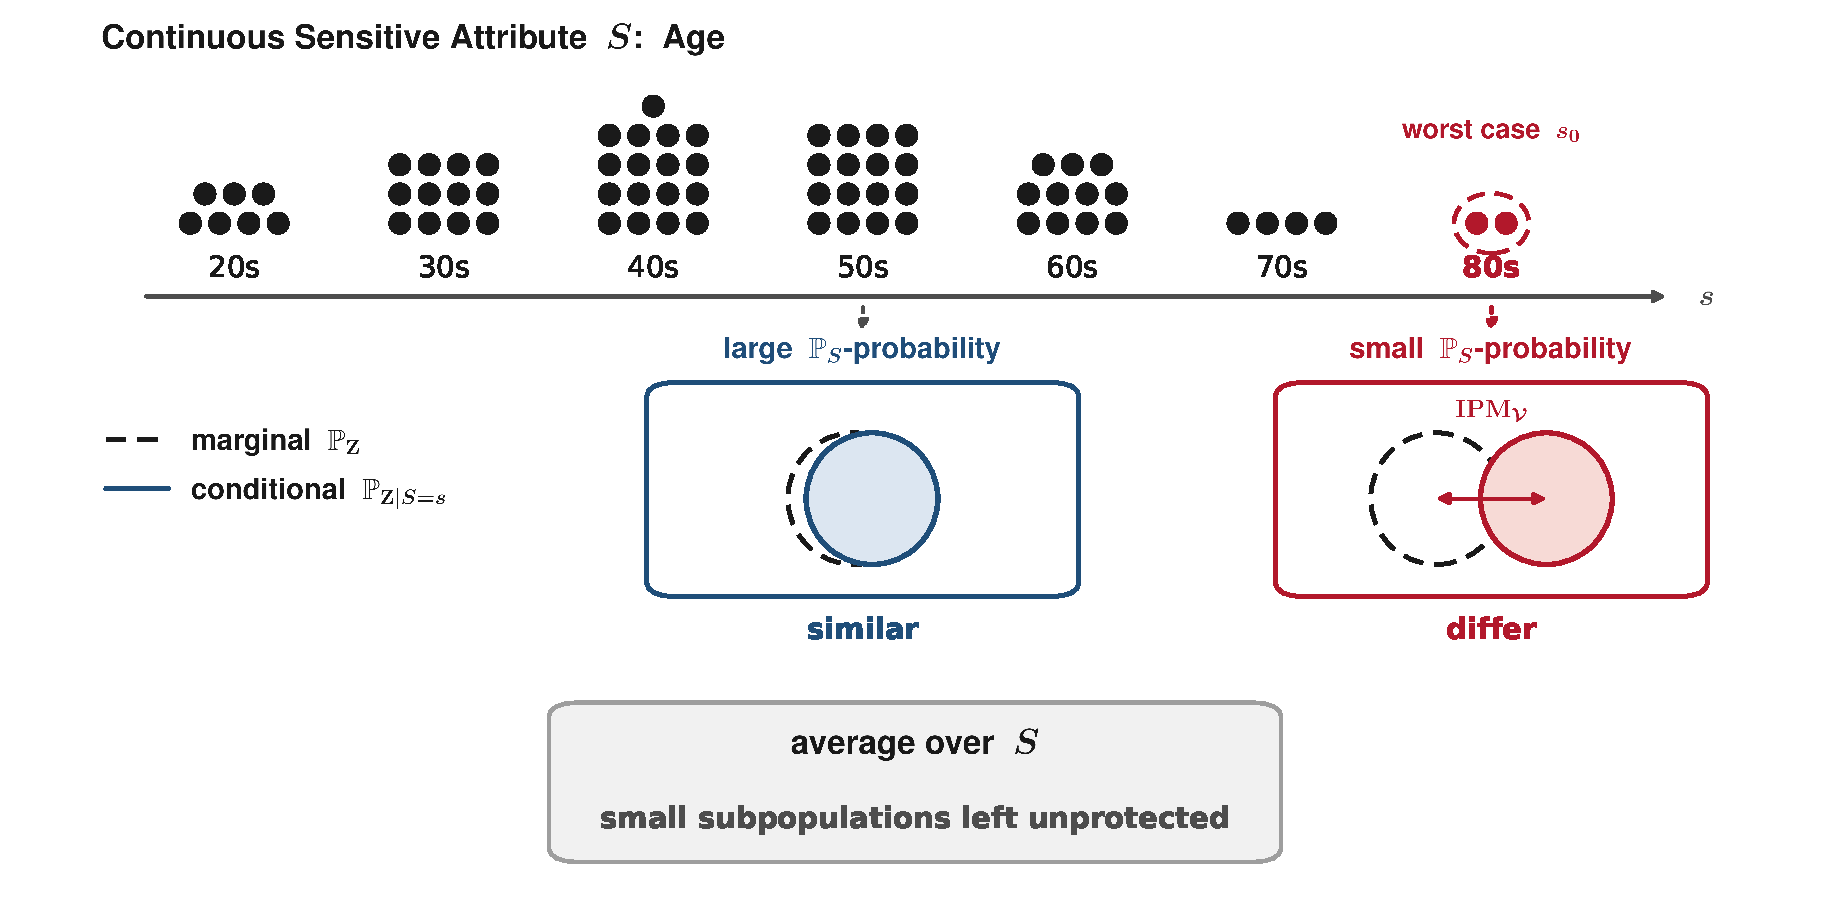
\includegraphics[width=0.8\textwidth]{motivation.pdf}
  \caption{The conditional and the marginal distribution of the representation coincide at a typical sensitive value and differ in a neighborhood of $s_0$.}
  \label{fig:motivation}
\end{figure}

Because the EIPM in (\ref{eq:eipm}) averages the IPM between $\mathbb{P}_{\mathbf{Z}\mid S=s}$ and $\mathbb{P}_{\mathbf{Z}}$ over $\mathbb{P}_S$, a large discrepancy of $\operatorname{IPM}_{\mathcal{V}}(\mathbb{P}_{\mathbf{Z}\mid S=s},\mathbb{P}_{\mathbf{Z}})$ at $s$ in a region of small $\mathbb{P}_S$-probability could contribute little to $\operatorname{EIPM}_{\mathcal{V}}(\mathbf{Z};S)$, and thus reducing  $\operatorname{EIPM}_{\mathcal{V}}(\mathbf{Z};S)$ may not reduce the $\operatorname{IPM}_{\mathcal{V}}(\mathbb{P}_{\mathbf{Z}\mid S=s},\mathbb{P}_{\mathbf{Z}})$ for all $s \in \mathcal{S}$.  
Figure~\ref{fig:motivation} illustrates such a case: $\operatorname{IPM}_{\mathcal{V}}(\mathbb{P}_{\mathbf{Z}\mid S=s},\mathbb{P}_{\mathbf{Z}})$ could be large at $s$ at which $\mathbb{P}_{S}$-probability is small even when $\operatorname{EIPM}_{\mathcal{V}}(\mathbf{Z};S)$ is small, because a small EIPM need not imply a small discrepancy at every sensitive value. 
To control $\operatorname{IPM}_{\mathcal{V}}(\mathbb{P}_{\mathbf{Z}\mid S=s},\mathbb{P}_{\mathbf{Z}})$ for all $s$, in this paper we take the supremum instead of the expectation with respect to $s$.
That is, we control $\sup_{s \in \mathcal{S}} \operatorname{IPM}_{\mathcal{V}}(\mathbb{P}_{\mathbf{Z}\mid S=s},\mathbb{P}_{\mathbf{Z}}) $ instead of EIPM.

%For $\operatorname{IPM}_{\mathcal{V}}(\mathbb{P}_{\mathbf{Z}\mid S=s},\mathbb{P}_{\mathbf{Z}})$ to be properly defined,
% , not only for $\mathbb{P}_S$-almost every $s$.  
% The positive-density assumption (as:positive-density), the joint density $p(\mathbf{x},s)$ and the conditional expectation (eq:pointwise-conditional) are stated in Appendix~\ref{app:assumptions}.
% chosen so that $\int_{\mathcal{X}} p(\mathbf{x},s)\,\mathrm{d}\nu(\mathbf{x})=p_S(s)$ for every $s\in\mathcal{S}$.
% Because a conditional expectation given $S=s$ is determined only up to a $\mathbb{P}_S$-null set of $s$,
% From this, a conditional expectation given $S=s$ is as follows
% As in Section~\ref{sec:frem}, the discriminator class $\mathcal{V}$ of this IPM specifies the prediction heads that the criterion controls.  
% With  $\mathbb{P}_{\mathbf{Z}\mid S=s}$ induced by the conditional density used in Equation~(\ref{eq:pointwise-conditional}), 
We define the supremum integral probability metric (supIPM) as
\begin{align}
  \operatorname{supIPM}_{\mathcal{V}}(\mathbf{Z};S)
  &:=\sup_{s\in\mathcal{S}}
  \operatorname{IPM}_{\mathcal{V}}
  \left(\mathbb{P}_{\mathbf{Z}\mid S=s},\mathbb{P}_{\mathbf{Z}}\right) \notag\\
  &=\sup_{s\in\mathcal{S}}\sup_{v\in\mathcal{V}}
  \left|
    \mathbb{E}\!\left[v(\mathbf{Z})\mid S=s\right]
    -\mathbb{E}\!\left[v(\mathbf{Z})\right]
  \right|.
  \label{eq:supipm}
\end{align}
By definition, the constraint $\operatorname{supIPM}_{\mathcal{V}}(\mathbf{Z};S)\le\rho$ for $\rho\ge0$ bounds 
$\operatorname{IPM}_{\mathcal{V}}(\mathbb{P}_{\mathbf{Z}\mid S=s},\mathbb{P}_{\mathbf{Z}})$ by $\rho$ at every $s\in\mathcal{S}$.
% and hence $\left|\mathbb{E}[v(\mathbf{Z})\mid S=s]-\mathbb{E}[v(\mathbf{Z})]\right|$ by the same $\rho$ for every discriminator $v\in\mathcal{V}$.  
Because the average never exceeds the supremum, $\operatorname{EIPM}_{\mathcal{V}}(\mathbf{Z};S)\le\operatorname{supIPM}_{\mathcal{V}}(\mathbf{Z};S)$, so a representation with a small supIPM also has a small EIPM.
% The converse fails without further regularity in $s$.
%In addition, if $f\in\mathcal{V}$, (\ref{eq:supipm}) bounds the difference between the conditional and the marginal means of its prediction $f(\mathbf{Z})$ by $\operatorname{supIPM}_{\mathcal{V}}(\mathbf{Z};S)$ at every $s\in\mathcal{S}.$  

For a bounded measurable function $g:\mathcal{X}\rightarrow \mathbb{R},$ \citet{jiang2022generalized} define generalized demographic parity (GDP) for a continuous sensitive attribute as
\begin{equation}
  \operatorname{GDP}(g)
  :=\mathbb{E}_{S}\!\left[
    \left|
      \mathbb{E}[g(\mathbf{X})\mid S]
      -\mathbb{E}[g(\mathbf{X})]
    \right|
  \right].
  \label{eq:gdp}
\end{equation}
For $g=f\circ h$, $\operatorname{GDP}(g)$ averages $\left|\mathbb{E}[f(\mathbf{Z})\mid S]-\mathbb{E}[f(\mathbf{Z})]\right|$ over $S$.  Replacing the average by the supremum, as in (\ref{eq:supipm}), we define $L_{\infty}$-generalized demographic parity ($\operatorname{GDP}_{\infty}$) as
\begin{equation}
  \operatorname{GDP}_{\infty}(g)
  :=\sup_{s\in\mathcal{S}}
  \left|
    \mathbb{E}[g(\mathbf{X})\mid S=s]
    -\mathbb{E}[g(\mathbf{X})]
  \right|.
  \label{eq:linfty-gdp}
\end{equation}
Note that $\operatorname{GDP}_{\infty}(f\circ h)\le\operatorname{supIPM}_{\mathcal{V}}(\mathbf{Z};S)$ as long as  $f\in\mathcal{V}$, 
and so we can control the fairness violation of $f(\mathbf{Z})$ for all $f\in \mathcal{V}$ 
in view of $\operatorname{GDP}(g)$ and $\operatorname{GDP}_{\infty}(g)$
by controlling $\operatorname{supIPM}_{\mathcal{V}}(\mathbf{Z};S)$.


\subsection{Choice of the Discriminator Class}
\label{sec:discriminator-choice}

It remains to choose the discriminator class $\mathcal{V}$.  
Note that $\operatorname{GDP}_{\infty}(f\circ h)$ for heads $f$ with a bounded H\"older norm is bounded by
$\operatorname{supIPM}_{\mathcal{H}^{\beta}_d}(\mathbf{Z};S).$
However, computation of $\operatorname{supIPM}_{\mathcal{H}^{\beta}_d}(\mathbf{Z};S)$
is not easy because function in $\mathcal{H}^{\beta}_d$ is not easily parameterizable.
To resolve this problem, we use ReLU-IPM, that is, we take $\mathcal{V}=\mathcal{V}_{\mathrm{R}}$ in (\ref{eq:supipm}) and control $\operatorname{supIPM}_{\mathcal{V}_{\mathrm{R}}}(\mathbf{Z};S)$. Since the discriminator class of ReLU-IPM has finite parameters,
computation of $\operatorname{supIPM}_{\mathcal{V}_{\mathrm{R}}}(\mathbf{Z};S)$ can be done without much hamper.
Moreover, the inequality (\ref{eq:relu-holder}) implies
that $\operatorname{GDP}_{\infty}(f\circ h)$ is bounded by $\operatorname{supIPM}_{\mathcal{V}_{\mathrm{R}}}(\mathbf{Z};S)$
under regularity conditions.

 % The H\"older-IPM cannot be computed directly, so we take $\mathcal{V}=\mathcal{V}_{\mathrm{R}}$, the ReLU discriminator class of Section~\ref{sec:relu-ipm}, for which the inner IPM in (\ref{eq:supipm}) is the ReLU-IPM.  
The ReLU-IPM is better than MMD from computational point of view.  
Computing EIPM with MMD requires $O(n^3)$ computation at each update.
In contrast, $\operatorname{supIPM}_{\mathcal{V}_{\mathrm{R}}}(\mathbf{Z};S)$ only needs $O(n)$ computation at each update.
Moreover, a mini-batch learning is not possible for EIPM with MMD \citep{lee2026fair}, and thus  
$O(n^2)$ memory is required. In contrast, we show in Appendix~\ref{app:mini-batch} that supIPM-FRL with the ReLU-IPM admits a mini-batch learning.

\subsection{Estimation of supIPM}
\label{sec:supipm-estimation}

%For the sample $\mathcal{D}$ of Section~\ref{sec:frem}, let $\mathbf{Z}_i=h_{\phi}(\mathbf{X}_i)$.  Estimating supIPM requires the conditional distribution $\mathbb{P}_{\mathbf{Z}\mid S=s}$ at every $s\in\mathcal{S}$, whereas FREM requires it only at the observed values $S_i$.  We therefore adapt the kernel-weighted construction of (\ref{eq:frem-conditional}) to an arbitrary $s$, for which the leave-one-out correction is not needed because $s$ is no longer tied to an observation:
Similar to EIPM, we can estimate $\operatorname{supIPM}_{\mathcal{V}_{\mathrm{R}}}(\mathbf{Z};S)$ by kernel techniques. Let
\begin{equation}
  \widehat{w}_{\gamma}(i;s)
  :=\frac{K_{\gamma}(S_i,s)}{\sum_{j=1}^n K_{\gamma}(S_j,s)},
  \quad
  \widehat{\mathbb{P}}^{\gamma}_{\mathbf{Z}\mid S=s}(\cdot)
  :=\sum_{i=1}^n\widehat{w}_{\gamma}(i;s)\,
  \delta_{\mathbf{Z}_i}(\cdot),
  \quad
  \widehat{\mathbb{P}}_{\mathbf{Z}}(\cdot)
  :=\frac{1}{n}\sum_{i=1}^n\delta_{\mathbf{Z}_i}(\cdot),
  \label{eq:supipm-estimators}
\end{equation}
where $K_{\gamma}$ is a given kernel.  We propose to estimate $\operatorname{supIPM}_{\mathcal{V}_{\mathrm{R}}}(\mathbf{Z};S)$ by
%The weights sum to one over $i$, so that $\widehat{\mathbb{P}}^{\gamma}_{\mathbf{Z}\mid S=s}$ is a probability distribution, and they place more weight on observations whose sensitive values are close to $s$.  Substituting the two empirical distributions into (\ref{eq:supipm}) yields
\begin{align}
  \widehat{\operatorname{supIPM}}^{\gamma}_{\mathcal{V}_{\mathrm{R}}}
  (\mathbf{Z};S)
  &:=\sup_{s\in\mathcal{S}}
  \operatorname{IPM}_{\mathcal{V}_{\mathrm{R}}}
  \left(\widehat{\mathbb{P}}^{\gamma}_{\mathbf{Z}\mid S=s},
        \widehat{\mathbb{P}}_{\mathbf{Z}}\right) \notag\\
  &=\sup_{s\in\mathcal{S}}
    \sup_{\theta\in\mathbb{S}^{d-1},\,\mu\in[-1,1]}
  \left|
    \sum_{i=1}^n
    \left(\widehat{w}_{\gamma}(i;s)-\frac{1}{n}\right)
    (\theta^\top\mathbf{Z}_i+\mu)_+
  \right|.
  \label{eq:empirical-supipm}
\end{align}
We prove in Theorem~\ref{thm:uniform} of Section~\ref{sec:theory} that this estimator converges to the population supIPM
with a properly chosen kernel and bandwidth.
%Unlike (\ref{eq:eipm-estimator}), (\ref{eq:empirical-supipm}) takes the largest estimated discrepancy over all of $\mathcal{S}$.  
% When $K_{\gamma}$ is differentiable, the weights are differentiable in $s$, so gradient ascent over $\mathcal{S}$ can maximize the discrepancy. 
%Section~\ref{sec:supipm-objective} introduces supIPM-FRL, which uses this empirical supIPM to learn representations with worst-case fairness control.

\subsection{Fair Representation Learning with supIPM}
\label{sec:supipm-objective}
%s^* 찾는 알고리즘 수정 처음엔 0.3 0.5 0.7 중에 큰거 0.7이 뽑혔으면 이제 0.6 0.7 0.8 중에 큰거. 0.6이 뽑혔으면 0.55 0.6 0.65 중 큰거... 이런식으로 찾는 알고리즘으로 수정.
% The empirical supIPM of Section~\ref{sec:supipm-estimation} measures the fairness of any encoder on the sample.  
To learn fair representations, we use the empirical supIPM of Section~\ref{sec:supipm-estimation} as a fairness penalty.
Let $h_{\phi}$ and $f_{\psi}$ be the encoder and the prediction head with parameters $\phi$ and $\psi$, respectively.
For $s\in\mathcal{S}$, $\theta\in\mathbb{S}^{d-1}$ and $\mu\in[-1,1]$, let
% To learn a fair representation with the supIPM, we add this estimate as a penalty to the supervised risk and train the encoder $h_{\phi}$ and the prediction head $f_{\psi}$ jointly by minimizing
\begin{equation}
  \mathcal{L}(\phi,\psi;s,\theta,\mu)
  :=\frac{1}{n}\sum_{i=1}^n
  \ell\!\left(f_{\psi}(h_{\phi}(\mathbf{X}_i)),Y_i\right)
  +\lambda\left|
    \sum_{i=1}^n
    \left(\widehat{w}_{\gamma}(i;s)-\frac{1}{n}\right)
    (\theta^\top h_{\phi}(\mathbf{X}_i)+\mu)_+
  \right|,
  \label{eq:supipm-penalized-objective}
\end{equation}
where $\ell$ is the supervised loss of Section~\ref{sec:frem} and $\lambda\ge0$ controls the accuracy--fairness trade-off.  
We jointly train the encoder and the prediction head by solving $\min_{\phi,\psi}\mathcal{L}(\phi,\psi)$ with $\mathcal{L}(\phi,\psi):=\sup_{s,\theta,\mu}\mathcal{L}(\phi,\psi;s,\theta,\mu)$.
% Equation~(\ref{eq:supipm-penalized-objective}) is the Lagrangian relaxation of minimizing the empirical supervised risk subject to $\widehat{\operatorname{supIPM}}^{\gamma}_{\mathcal{V}_{\mathrm{R}}}(\mathbf{Z};S)\le\rho$, as in Section~\ref{sec:supipm-criterion}.
Since $\lambda\ge0$, this problem is a penalized formulation of empirical supervised risk minimization subject to $\widehat{\operatorname{supIPM}}^{\gamma}_{\mathcal{V}_{\mathrm{R}}}(\mathbf{Z};S)\le\rho$.

% , so the minimization of Equation~(\ref{eq:supipm-penalized-objective}) is a min--max problem.  
% We solve it by alternating gradient descent in $(\phi,\psi)$ with compass search \citep{kolda2003optimization} in $s$ and projected gradient ascent in $(\theta,\mu)$, which extends the computation of ReLU-IPM in \citet{park2026relu} to the additional supremum over $s$. 
To optimize this objective function, we alternate between two steps.
With $(\phi,\psi)$ fixed, we approximate the supremum over $(s,\theta,\mu)$ in $\mathcal{L}(\phi,\psi)$ by compass search over $s$ \citep{kolda2003optimization} and projected gradient ascent over $(\theta,\mu)$.
With $(s,\theta,\mu)$ fixed, we update $(\phi,\psi)$ by gradient descent on $\mathcal{L}(\phi,\psi;s,\theta,\mu)$ in Equation~(\ref{eq:supipm-penalized-objective}).
% This optimization scheme extends the computation of ReLU-IPM in \citet{park2026relu} by additionally maximizing over $s$.
Because the compass search and the gradient ascent can converge to a local maximum, we use $T$ initial values of $s$ and $M$ discriminator initializations.  
We refer to this training method as supIPM-FRL, which can be implemented efficiently using mini-batches (Appendix~\ref{app:mini-batch}).  Further details and the algorithms are provided in  Appendices~\ref{app:ascent} and ~\ref{app:algorithm-steps}, respectively.

Section~\ref{sec:theory} shows that, with high probability, a small empirical supIPM yields a small $\operatorname{GDP}_{\infty}$ on an interior region of $\mathcal{S}$ for every downstream head of bounded H\"older norm.

\begin{remark}[Multivariate sensitive attributes]
\label{rem:multivariate-sensitive}
For $S\in\mathcal{S}\subset\mathbb{R}^r$ with $r>1$, we use a multivariate kernel 
\begin{equation*}
    K_{\gamma}(s',s)=\gamma^{-r}\prod_{k=1}^r K((s'_k-s_k)/\gamma)
\end{equation*}
where $K(\cdot)$ is a univariate kernel in (\ref{eq:supipm-estimators}).
We approximate the supremum in (\ref{eq:empirical-supipm}) by compass search over $\mathcal{S}$  along each coordinate, together with projected gradient ascent over $(\theta,\mu)$.
With $T$ initial candidate vectors, each compass search iteration evaluates at most $T(2r+1)$ sensitive values \citep{kolda2003optimization}.
Thus, for fixed $T$, the number of evaluations per iteration grows linearly with $r$, making supIPM-FRL straightforward to extend to multivariate sensitive attributes without hampering computation.
\end{remark}


\section{Theoretical Analysis}
\label{sec:theory}

% supIPM-FRL of Section~\ref{sec:supipm-objective} learns the encoder by penalizing the empirical supIPM, whereas the fairness of the learned representation is measured by the population supIPM.  
Theorem~\ref{thm:uniform} establishes uniform convergence of the empirical
supIPM to its population counterpart over a class of encoders.
Corollary~\ref{cor:certificate} then bounds the $\operatorname{GDP}_{\infty}$ of prediction heads of bounded H\"older norm in terms of the empirical supIPM, as stated at the end of Section~\ref{sec:supipm-objective}.

Theorem~\ref{thm:uniform} and Corollary~\ref{cor:certificate} are stated on the interior region $\mathcal{S}_n:=[\epsilon_n,1-\epsilon_n]$ of $\mathcal{S}=[0,1]$, where $0<\epsilon_n<\tfrac{1}{2}$ and $\epsilon_n\to0$.  We restrict the suprema over $s$ in Equations~(\ref{eq:supipm}),~(\ref{eq:linfty-gdp}), and~(\ref{eq:empirical-supipm}) to $\mathcal{S}_n$ and set $\gamma=\gamma_n$ for the empirical supIPM in (\ref{eq:empirical-supipm}). This gives
\begin{equation}
\begin{aligned}
  \operatorname{GDP}_{\infty,n}(g)
  &:=\sup_{s\in\mathcal{S}_n}
     \left|\mathbb{E}[g(\mathbf{X})\mid S=s]-\mathbb{E}[g(\mathbf{X})]\right|,
  \\
  \operatorname{supIPM}_{\mathcal{V}_{\mathrm{R}},n}(h(\mathbf{X});S)
  &:=\sup_{s\in\mathcal{S}_n}
     \operatorname{IPM}_{\mathcal{V}_{\mathrm{R}}}
     \bigl(\mathbb{P}_{h(\mathbf{X})\mid S=s},
           \mathbb{P}_{h(\mathbf{X})}\bigr),
  \\
  \widehat{\operatorname{supIPM}}^{\gamma_n}_{\mathcal{V}_{\mathrm{R}},n}(h(\mathbf{X});S)
  &:=\sup_{s\in\mathcal{S}_n}
     \operatorname{IPM}_{\mathcal{V}_{\mathrm{R}}}
     \bigl(\widehat{\mathbb{P}}^{\gamma_n}_{h(\mathbf{X})\mid S=s},
           \widehat{\mathbb{P}}_{h(\mathbf{X})}\bigr).
\end{aligned}
  \label{eq:interior}
\end{equation}
To bound the difference between $\widehat{\operatorname{supIPM}}^{\gamma_n}_{\mathcal{V}_{\mathrm{R}},n}(h(\mathbf{X});S)$ and $\operatorname{supIPM}_{\mathcal{V}_{\mathrm{R}},n}(h(\mathbf{X});S)$ uniformly over a class $\mathcal{E}_n$ of encoders, we assume four conditions, stated in Appendix~\ref{app:assumptions}.  Assumption~\ref{as:positive-density} requires $\mathbb{P}_S$ to have a density $p_S$ with $0<c_S\le p_S\le C_S<\infty$ on $\mathcal{S}$.  Assumption~\ref{as:smooth-density} requires a joint density of $(\mathbf{X},S)$ that is twice continuously differentiable in $s$, with integrable envelopes $M_1$ and $M_2$.  Assumption~\ref{as:kernel} requires a bounded, symmetric and Lipschitz kernel $K$ in $K_{\gamma}(s',s)=\gamma^{-1}K((s'-s)/\gamma)$, together with a bandwidth $\gamma_n\to0$.
% that is at most $\min\{\epsilon_n,1/2\}$ and for which the kernel centered at any $s\in\mathcal{S}_n$ places mass at most $\gamma_n^2$ outside $\mathcal{S}$.  
Assumption~\ref{as:encoder} requires the encoder class $\mathcal{E}_n$ have covering number at most $(A_n/\eta)^{\mathfrak{v}_n}$ in the supremum norm at every radius $\eta\in(0,1]$.  
To state the uniform convergence rate, let $0<\delta<1$ and define
\begin{equation}
  \Gamma_{n,\delta}
  :=(\mathfrak{v}_n+d)\log\frac{A_nn}{\gamma_n}+\log\frac{1}{\delta},
  \qquad
  r_{n,\delta}
  :=\gamma_n^2+\sqrt{\frac{\Gamma_{n,\delta}}{n\gamma_n}} .
  \label{eq:rate}
\end{equation}

\begin{theorem}[Uniform convergence rate of the empirical supIPM]
\label{thm:uniform}
Let Assumptions~\ref{as:positive-density}--\ref{as:encoder} hold.  There exist constants $C,c>0$, depending only on $c_S$, $C_S$, $K$, $\lVert M_1\rVert_{L_1(\nu)}$ and $\lVert M_2\rVert_{L_1(\nu)}$, such that for every $\delta\in(0,1)$ and every $n$ with $\Gamma_{n,\delta}\le c\,n\gamma_n$, with probability at least $1-\delta$,
\begin{equation}
  \sup_{h\in\mathcal{E}_n}
  \left|\widehat{\operatorname{supIPM}}^{\gamma_n}_{\mathcal{V}_{\mathrm{R}},n}(h(\mathbf{X});S)-\operatorname{supIPM}_{\mathcal{V}_{\mathrm{R}},n}(h(\mathbf{X});S)\right|
  \ \le\ C\,r_{n,\delta} .
  \label{eq:uniform}
\end{equation}
If in addition $A_n$ and $\mathfrak{v}_n$ are bounded, $\delta:=\delta_n=n^{-c_1}$ for some $c_1>0$, $\gamma_n\asymp(\log n/n)^{1/5}$ and $\epsilon_n\asymp1/\log n$, then $r_{n,\delta_n}=O\{(\log n/n)^{2/5}\}$.
\end{theorem}

Theorem~\ref{thm:uniform} shows that the fairness level attained on the sample over $\mathcal{S}_n$ transfers to the population over $\mathcal{S}_n$.  If $\widehat{\operatorname{supIPM}}^{\gamma_n}_{\mathcal{V}_{\mathrm{R}},n}(h(\mathbf{X});S)\le\rho$ for an encoder $h\in\mathcal{E}_n$, then $\operatorname{supIPM}_{\mathcal{V}_{\mathrm{R}},n}(h(\mathbf{X});S)\le\rho+Cr_{n,\delta}$ with probability at least $1-\delta$.  
The bound is uniform over $\mathcal{E}_n$, so it applies to the encoder that supIPM-FRL obtains from the same sample.  
% Because $D_n(h)$ is a supremum over $\mathcal{S}_n$, the transfer holds at every sensitive value in $\mathcal{S}_n$ rather than on average.  
% One may expect the supremum over the sensitive domain and the representation dimension $d$ to slow the convergence.  The supremum enters $r_{n,\delta}$ only through the logarithmic factor in $\Gamma_{n,\delta}$, and $d$ enters $\Gamma_{n,\delta}$ linearly because $\mathcal{V}_{\mathrm{R}}$ is indexed by $d+1$ parameters, so the order of $r_{n,\delta}$ in $n$ is unchanged.  For an encoder class of bounded size, the bandwidth $\gamma_n\asymp(\log n/n)^{1/5}$ gives the rate $(\log n/n)^{2/5}$ of Theorem~\ref{thm:uniform}.
% For bounded $A_n$ and $\mathfrak{v}_n$, the bandwidth $\gamma_n\asymp(\log n/n)^{1/5}$ gives the rate $(\log n/n)^{2/5}$.  
% This is the minimax rate for uniformly estimating a twice differentiable regression function on an interval \citep{stone1982optimal}, so the supremum over $s$ and the dimension $d$ do not slow the convergence in $n$.
Moreover, since $\epsilon_n \to 0$, $\mathcal{S}_n$ expands toward the boundary as the sample size grows, so every fixed sensitive value in the interior of $\mathcal{S}$ is eventually covered.


Theorem~\ref{thm:uniform} and inequality in (\ref{eq:relu-holder}) yield the following corollary.  For $B>0$ let $\mathcal{H}^{\beta}_d(B)$ be the H\"older ball of (\ref{eq:holder-ball}) with radius $B$, and let $C_{d,\beta}$ and $\alpha_{d,\beta}$ be the constant and exponent in (\ref{eq:relu-holder}), so that $\alpha_{d,\beta}=2\beta/(d+3)$ for $\beta<(d+3)/2$ and $\alpha_{d,\beta}=1$ for $\beta>(d+3)/2$.
\begin{corollary}
\label{cor:certificate}
Let Assumptions~\ref{as:positive-density}--\ref{as:encoder} hold, let $d\ge3$, and let $C$ and $c$ be the constants of Theorem~\ref{thm:uniform}.  For every $\delta\in(0,1)$ and  $n$ with $\Gamma_{n,\delta}\le c\,n\gamma_n$, with probability at least $1-\delta$, simultaneously for all  $h\in\mathcal{E}_n$,  $B>0$ and  $\beta>0$ with $\beta\ne(d+3)/2$,
\begin{equation}
  \sup_{f\in\mathcal{H}^{\beta}_d(B)}
  \operatorname{GDP}_{\infty,n}(f\circ h)
  \ \le\ C_{d,\beta}\,B
  \left\{\widehat{\operatorname{supIPM}}^{\gamma_n}_{\mathcal{V}_{\mathrm{R}},n}(h(\mathbf{X});S)+Cr_{n,\delta}\right\}^{\alpha_{d,\beta}} .
  \label{eq:certificate}
\end{equation}
\end{corollary}
% This corollary shows that by learning an encoder $h$ with a small $\widehat{\operatorname{supIPM}}^{\gamma_n}_{\mathcal{V}_{\mathrm{R}},n}(h(\mathbf{X});S)$, supIPM-FRL controls the fairness violation $\operatorname{GDP}_{\infty,n}(f\circ h)$ uniformly over all prediction heads $f\in\mathcal{H}^{\beta}_d(B)$.
This corollary shows that by learning an encoder $h$ with a small empirical supIPM, supIPM-FRL controls the worst-case fairness violation over all prediction heads $f\in\mathcal{H}^{\beta}_d(B)$.


% Thus $\widehat{\operatorname{supIPM}}^{\gamma_n}_{\mathcal{V}_{\mathrm{R}},n}(h(\mathbf{X});S)$ bounds $\operatorname{GDP}_{\infty,n}(f\circ h)$, and hence $\left|\mathbb{E}[f(\mathbf{Z})\mid S=s]-\mathbb{E}[f(\mathbf{Z})]\right|$ at every $s\in\mathcal{S}_n$, uniformly over all heads $f\in\mathcal{H}^{\beta}_d(B)$.
% The right-hand side of Equation~(\ref{eq:certificate}) depends on neither the sensitive value nor the prediction head, and the bound holds simultaneously over $\mathcal{E}_n$, so the single quantity $\widehat{D}_n(h)$ controls the $\operatorname{GDP}_{\infty}$ of every H\"older prediction head over $\mathcal{S}_n$.  
% The exponent $\alpha_{d,\beta}$ is the cost of measuring the discrepancy through the parametric class $\mathcal{V}_{\mathrm{R}}$ rather than through the H\"older ball itself, and equals one when $\beta>(d+3)/2$.


\section{Experiments}
\label{sec:experiments}

% This section evaluates supIPM-FRL on simulated data, where the location $s_0$ of the dependence on $S$ is known, and on three tabular datasets, where we compare it with existing baselines. 
This section evaluates supIPM-FRL on simulated data and three tabular datasets.
Experimental details are given in Appendices~\ref{app:synth-experiments} and~\ref{app:real-experiments}.

\paragraph{Measures.}  Prediction performance is the test accuracy for classification and the test $1-\mathrm{MAE}$ for regression.  Fairness is measured through the disparity of a prediction head $f$ at each sensitive value:
\begin{equation}
    \Delta_{f}(s):=|\mathbb{E}[f(\mathbf{Z})\mid S=s]-\mathbb{E}[f(\mathbf{Z})]|.
\end{equation}
% whose supremum over $s$ is $\operatorname{GDP}_{\infty}(f\circ h)$ of Equation~(\ref{eq:linfty-gdp}).  
The prediction-level disparity is $\operatorname{GDP}_{\infty}(f_{\psi}\circ h_{\phi}) = \sup_{s} \Delta_{f_{\psi}}(s)$ for the head trained jointly with the encoder.  Since a representation may later serve other heads \citep{coston2021characterizing,jovanovic2023fare,luo2026fair}, we also measure the largest disparity that a downstream head can attain.  For $c>0$, let $\mathcal{F}_c:=\{\sigma(\mathbf{w}^\top\mathbf{z}+b):\lVert\mathbf{w}\rVert_2\le c,\ b\in\mathbb{R}\}$ be the logistic heads with weight norm at most $c$, where $\sigma(t):=(1+e^{-t})^{-1}$, and define the worst-case disparity as
\begin{equation}
  \operatorname{GDP}_{\infty}(h_{\phi};\mathcal{F}_c):=\sup_{f\in\mathcal{F}_c}\operatorname{GDP}_{\infty}(f\circ h_{\phi}) = \sup_{f\in\mathcal{F}_c} \sup_{s \in \mathcal{S}} \Delta_{f}(s).
  \label{eq:worst-case-gdp}
\end{equation}
% Every head in $\mathcal{F}_c$ has a bounded H\"older norm, so Corollary~\ref{cor:certificate} bounds Equation~(\ref{eq:worst-case-gdp}) in terms of the empirical supIPM.  
% All disparities are reported as kernel estimates on the test data; 
$\widehat{\Delta}_{f}$ and $\widehat{\operatorname{GDP}}_{\infty}$ denote these estimates and are defined in Appendix~\ref{app:worst-case}.

\paragraph{Estimating the worst-case disparity.}  With the encoder held fixed, write $f_{\mathbf{w},b}(\mathbf{z}):=\sigma(\mathbf{w}^\top\mathbf{z}+b)$ and, on the training data, minimize
\begin{equation}
  \widetilde{\mathcal{L}}(\mathbf{w},b)
  :=\frac{1}{n}\sum_{i=1}^n
  \ell\!\left(f_{\mathbf{w},b}(\mathbf{Z}_i),Y_i\right)
  -\lambda_h\,
  \widehat{\operatorname{GDP}}_{\infty}(f_{\mathbf{w},b}\circ h_\phi)
  \label{eq:worst-case-estimate}
\end{equation}
over $\lVert\mathbf{w}\rVert_2\le c$ and $b\in\mathbb{R}$, with $\lambda_h=10^{3}$ so that the disparity term dominates.  The minimizer $\hat{f}_c$ approximates the head attaining the supremum in Equation~(\ref{eq:worst-case-gdp}), and the worst-case disparity is estimated on the test data by $\widehat{\operatorname{GDP}}_{\infty}(h_\phi;\mathcal{F}_c):=\widehat{\operatorname{GDP}}_{\infty}(\hat{f}_c\circ h_\phi)$.

\subsection{Simulation study}
\label{sec:exp-simulation}



\paragraph{Setup.}  
% $S$ is uniform on an interval; the outcome $Y$ and one input variable depend on $S$ through a term concentrated near a value $s_0$, so that this dependence is confined to a set of small $\mathbb{P}_S$-probability, and $Y$ and a second input variable also depend on $S$ linearly; the generating equations are given in Appendix~\ref{app:synth-experiments}. 
% With $S$ uniformly distributed on an interval, the outcome $Y$ and one input variable depend on $S$ through a term localized near $s_0$ in a region of small $\mathbb{P}_S$-probability.
% The outcome $Y$ and a second input variable also depend linearly on $S$, with the full data-generating process specified in Appendix~\ref{app:synth-experiments}.
Let $S\sim\mathrm{Uniform}(0,1)$ and $\mathbf{X}=(\mathbf{X}_{\mathrm{task}},X_{\mathrm{loc}},\mathbf{X}_{\mathrm{noise}})$, where $\mathbf{X}_{\mathrm{task}}\in\mathbb{R}^4$ and $\mathbf{X}_{\mathrm{noise}}\in\mathbb{R}^3$ are standard normal and independent of $S$, and
\begin{equation*}
  X_{\mathrm{loc}}:=3\exp\!\left\{-\frac{(S-s_0)^2}{2\tau^2}\right\}+0.5\,\varepsilon_1,
  \qquad
  Y:=\sigma\!\left(\mathbf{u}^\top\mathbf{X}_{\mathrm{task}}+0.3\,\varepsilon_2\right),
\end{equation*}
with $s_0=0.5$, $\tau=0.043$, standard normal $\varepsilon_1,\varepsilon_2$ and a fixed $\mathbf{u}$.  
% Thus $\mathbf{X}$ depends on $S$ only through $X_{\mathrm{loc}}$, which is shifted only for $S$ near $s_0$, and $Y$ does not depend on $S$. 
A representation that depends on $X_{\mathrm{loc}}$ therefore differs from its marginal distribution mainly for $S$ near $s_0$.
The remaining settings are given in Appendix~\ref{app:synth-experiments}.
We compare supIPM-FRL with FREM over a grid of penalty parameters, using the worst-case downstream disparity over $\mathcal{F}_1$ as the fairness measure. 
% Each curve joins the configurations in increasing order of the penalty parameter.

\begin{figure}[!h]
  \centering
  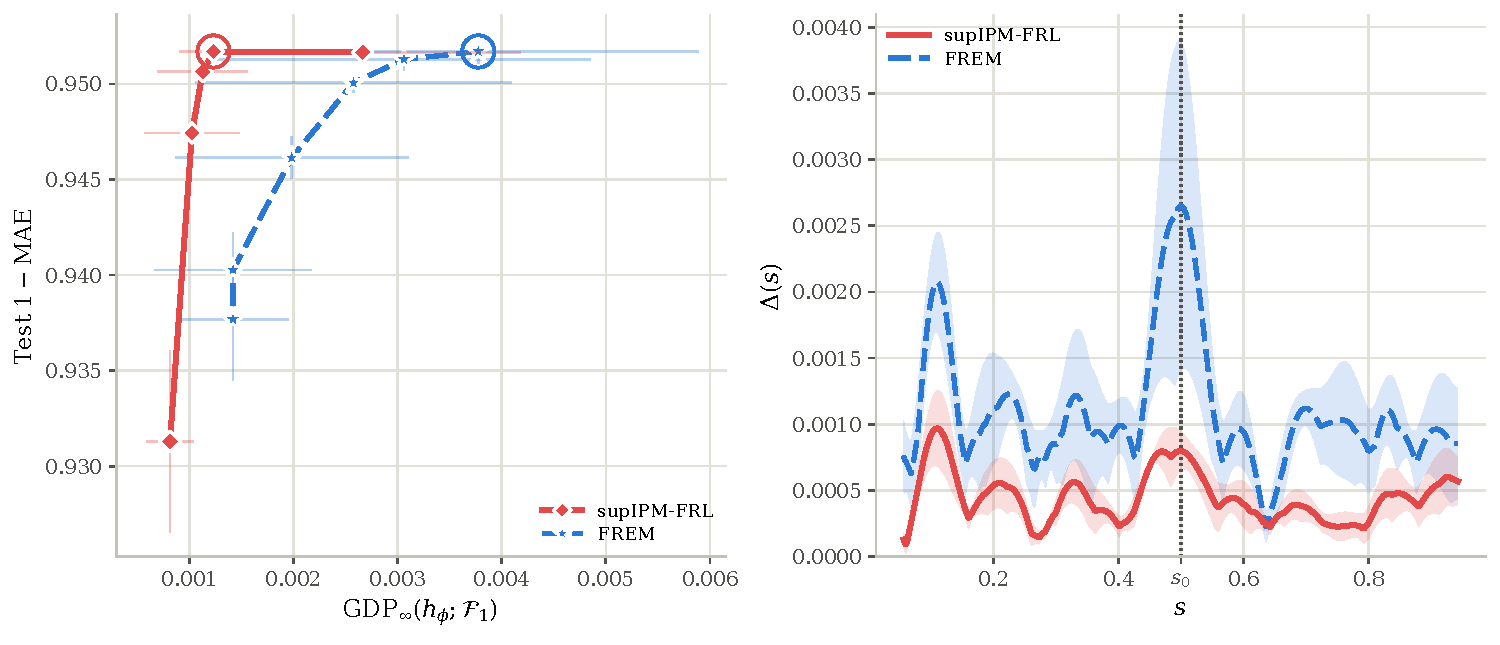
\includegraphics[width=0.8\textwidth]{main/fig1_simulation.pdf}
  \caption{Left: prediction performance against $\widehat{\operatorname{GDP}}_{\infty}(h_{\phi};\mathcal{F}_1)$; the upper left is favorable.  Right: $\widehat{\Delta}_{\hat{f}_1}(s)$  at the two circled points.}
  \label{fig:simulation}
\end{figure}

\paragraph{Results.}  In the left panel of Figure~\ref{fig:simulation}, supIPM-FRL achieves lower disparity than FREM at matched prediction performance.
% Because $Y$ does not depend on $S$, the dependence near $s_0$ can be removed without giving up prediction performance, and the left panel shows that supIPM-FRL does remove it: its curve runs horizontally before it turns downward. The right panel shows what each penalty leaves behind. 
The circled points are the configurations with the smallest disparity that retain the prediction performance of the model trained without a penalty.  At these points FREM still exhibits a peak in $\widehat{\Delta}_{\hat{f}_1}(s)$ at $s_0$, whereas the $\widehat{\Delta}_{\hat{f}_1}(s)$ of supIPM-FRL at $s_0$ is markedly smaller. 
This is the situation of Figure~\ref{fig:motivation}. 
The region near $s_0$ has low probability and therefore contributes little to the average in Equation~(\ref{eq:eipm}).
Consequently, the representation obtained by FREM may retain dependence localized near $s_0$.
In contrast,  the supremum in Equation~(\ref{eq:supipm}) is attained near $s_0$, so supIPM-FRL controls this dependence directly. 



\subsection{Real data analysis}
\label{sec:exp-real}

\paragraph{Datasets.}  We use three tabular datasets.
\begin{itemize}[leftmargin=*, itemsep=0pt, topsep=2pt]
  \item Adult \citep{adult_2}: $Y$ is whether income exceeds \$50k and $S$ is age.
  \item Crime \citep{communities_and_crime_183}: $Y$ is the violent crime rate and $S$ is the proportion of Black residents.
  \item ACSIncome \citep{ding2021retiring}: $Y$ is income in the 2018 American Community and $S$ is age.
\end{itemize}
Table~\ref{tab:datasets} in Appendix~\ref{app:real-experiments} gives further details, and results on the graph datasets Pokec-z and Pokec-n \citep{takac2012data} are also provided there.

\paragraph{Baselines.}  
Four baselines use the continuous $S$ directly.
FREM \citep{kong2025fair} is described in Section~\ref{sec:frem}.
Reg-GDP \citep{jiang2022generalized} penalizes predictions using GDP in Equation~(\ref{eq:gdp}).
Reg-HGR \citep{mary2019fairness} uses the Hirschfeld--Gebelein--Renyi (HGR) maximal correlation as the prediction penalty.
ADV \citep{zhang2018mitigating,kong2025fair} trains an adversary to predict $S$ from the representation.
The other three, LAFTR \citep{madras2018learning}, MMD \citep{deka2023mmd} and sIPM-LFR \citep{kim2022learning}, are FRL methods for a categorical sensitive attribute. They are applied to $S$ discretized at its median.  
All methods share the architecture of Appendix~\ref{app:real-settings} and are trained over a grid of penalty parameters with five random seeds.

\begin{figure}[!htb]
  \centering
  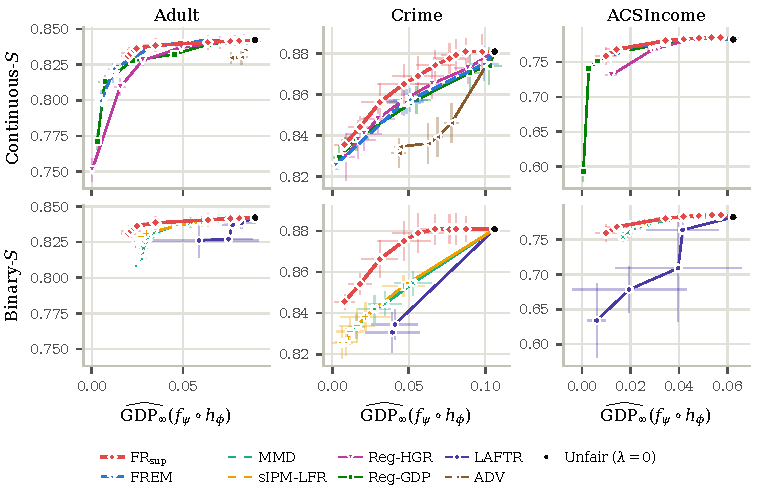
\includegraphics[width=0.92\textwidth]{main/fig2g_own_head_all.pdf}
  \vspace{-10pt}
  \caption{Prediction performance against the prediction-level disparity $\widehat{\operatorname{GDP}}_{\infty}(f_{\psi}\circ h_{\phi})$.}
  \label{fig:adult}
  \vspace{-4pt}
\end{figure}

\paragraph{Results.}  
% Each point is the mean over five seeds with bars of $\pm1$ standard deviation, each curve traces the configurations of one method with the smallest disparity at each level of prediction performance, and the upper left is favorable. 
Figure~\ref{fig:adult} shows the prediction-level disparity and Figure~\ref{fig:worst-case} the worst-case downstream disparity over $\mathcal{F}_1$ on the three datasets.
% the results with $S$ discretized at its mean and the worst-case curves over $\mathcal{F}_4$ and $\mathcal{F}_8$ are given in Appendix~\ref{app:real-tabular}.  
At the prediction level, supIPM-FRL is comparable to the other methods.  Under the worst-case downstream disparity, supIPM-FRL attains a markedly smaller disparity than every other method at the same prediction performance on all three datasets.
% , where the methods that use $S$ directly coincide with it.

\begin{figure}[!htb]
  \centering
  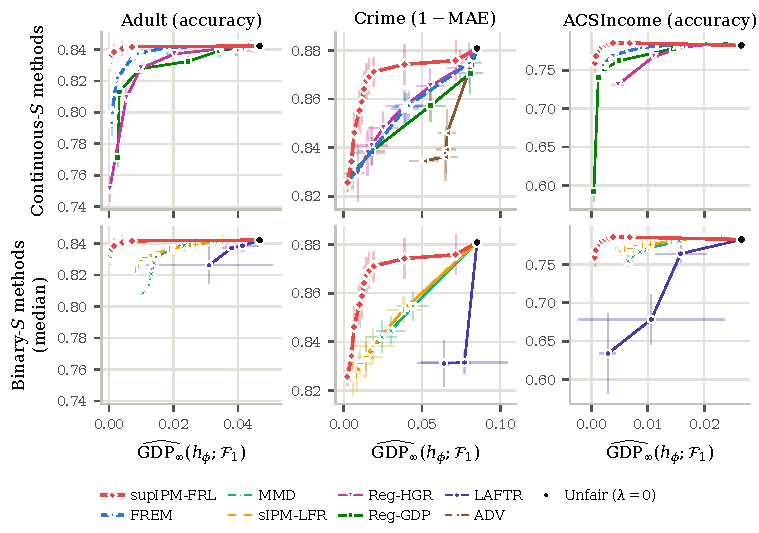
\includegraphics[width=0.92\textwidth]{main/fig3g_worst_head_all.pdf}
  \vspace{-10pt}
  \caption{Prediction performance against the worst-case downstream disparity $\widehat{\operatorname{GDP}}_{\infty}(h_{\phi};\mathcal{F}_1)$.}
  \label{fig:worst-case}
  \vspace{-4pt}
\end{figure}

The prediction-level disparity concerns the trained head only, whereas the worst-case disparity concerns every head in $\mathcal{F}_1$.  
% The other methods constrain the dependence on $S$ only on average over $S$, only within groups of a discretized $S$, or only through a single head or adversary, so a downstream head can use the dependence they leave.
The baselines do not directly control the dependence between the representation and $S$ at every sensitive value. 
They may therefore achieve low disparity for the trained head while the representation still depends on $S$. 
Another downstream head can exploit that dependence, which raises the worst-case disparity.
\Needspace{11\baselineskip}
\begin{wrapfigure}{r}{0.38\textwidth}
  \vspace{-9pt}
  \centering
  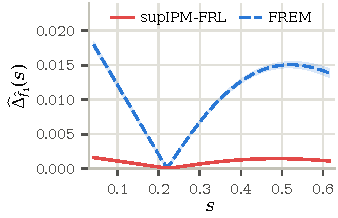
\includegraphics[width=\linewidth]{main/fig5_profile_adult.pdf}
  \vspace{-14pt}
  \caption{$\widehat{\Delta}_{\hat{f}_1}(s)$  of supIPM-FRL and FREM at matched test accuracy.}
  \label{fig:profile-adult}
  \vspace{-10pt}
\end{wrapfigure}

In contrast, supIPM-FRL controls the largest ReLU-IPM between $\mathbb{P}_{\mathbf{Z}\mid S=s}$ and $\mathbb{P}_{\mathbf{Z}}$ over the sensitive domain, and Corollary~\ref{cor:certificate} bounds $\Delta_f(s)$ at every $s$ in the interior region $\mathcal{S}_n$ for every head $f$ of bounded H\"older norm in terms of the empirical supIPM.
Figure~\ref{fig:profile-adult} shows $\widehat{\Delta}_{\hat{f}_1}(s)$ of supIPM-FRL and FREM on Adult. We consider settings with test accuracy within $0.004$ of the baseline accuracy at $\lambda=0$. For each method, we take the setting with the smallest worst-case disparity among these settings. At comparable test accuracy, $\widehat{\Delta}_{\hat{f}_1}(s)$ of supIPM-FRL is small across the sensitive domain, whereas that of FREM is substantially larger.
  
  % on Adult for the configurations with the smallest worst-case disparity among those whose test accuracy is within $0.004$ of the model trained without a penalty. the worst-case head of FREM attains a disparity many times larger than that of supIPM-FRL, whose disparity is small at every $s$.  Accordingly, the empirical supIPM on the test data in Appendix~\ref{app:real-measures} is smallest for supIPM-FRL on Adult and Crime at a matched level of prediction performance, although FREM attains a smaller value on ACSIncome.


\subsection{Ablation studies and additional results}

Appendix~\ref{app:real-measures} compares the methods under five further fairness measures, and Appendix~\ref{app:real-graph} compares them on the graph datasets.  The computational cost is reported in Appendix~\ref{app:real-cost}.  Appendix~\ref{app:ablation-studies} ablates two choices in the penalty, (i) the shape of the smoothing kernel and (ii) the class of the discriminators.

\section{Conclusion}
\label{sec:conclusion}

% Existing fairness criteria for a continuous sensitive attribute average the discrepancy between the conditional and the marginal distribution over the sensitive attribute, so that such criteria can obscure large discrepancies in low-probability regions of the sensitive domain.  
% We proposed $\operatorname{GDP}_{\infty}$ and supIPM, which replace the average by a supremum over the sensitive domain and thereby impose one fairness level at every sensitive value.  supIPM-FRL estimates the supIPM from kernel weights and ReLU discriminators and searches the sensitive domain for the largest discrepancy.  We proved that the empirical supIPM converges uniformly to its population counterpart at the rate of nonparametric regression, so that the fairness level attained on the sample transfers to the population, and that this single quantity bounds the $\operatorname{GDP}_{\infty}$ of every prediction head of bounded H\"older norm.  
% On simulated and real data, supIPM-FRL achieves prediction performance and prediction-level disparity comparable to those of existing methods, while substantially reducing worst-case disparity over downstream heads.

% Two directions remain: extending supIPM to a multivariate or mixed sensitive attribute, for which the supremum ranges over a multidimensional domain, and finding a discriminator class that controls H\"older heads with an exponent closer to one than $\alpha_{d,\beta}$ in Equation~(\ref{eq:relu-holder}) while remaining computable.


We proposed supIPM, which measures the worst-case fairness violation of a representation for a continuous sensitive attribute by the supremum over the sensitive domain of the IPM between the conditional and the marginal distributions, and supIPM-FRL, which uses the empirical supIPM as a fairness penalty.
We established a uniform convergence rate of the empirical supIPM over a class of encoders and showed that it bounds the $\operatorname{GDP}_{\infty}$ of every prediction head of bounded H\"older norm over the interior region $\mathcal{S}_n$.
With the ReLU discriminator class, supIPM-FRL admits a mini-batch formulation with unbiased gradients for fixed inner variables.
On simulated and real data, supIPM-FRL attains a markedly smaller worst-case downstream disparity than existing methods at comparable prediction performance.

% Future work includes extending supIPM-FRL to multivariate sensitive attributes.
% We also aim to support training when sensitive attributes are observed for only some samples.

\newpage

\bibliographystyle{iclr2027_conference}
\bibliography{bibliography}

\newpage
\appendix
\begin{center}
    {\LARGE \textsc{Appendix}}
\end{center}
\crefalias{section}{appendix}
\crefalias{subsection}{appendix}
\section{Proofs of the Main Results}
\label{app:proofs}

This appendix states the assumptions of Section~\ref{sec:theory}, proves four auxiliary lemmas, and then proves Theorem~\ref{thm:uniform} and Corollary~\ref{cor:certificate}.

\subsection{Assumptions}
\label{app:assumptions}

We state the four conditions imposed in Section~\ref{sec:theory}, with $\mathcal{S}=[0,1]$ as in Section~\ref{sec:frem} and $\mathcal{S}_n$, $\epsilon_n$ and $\gamma_n$ as in Section~\ref{sec:theory}.

\begin{assumption}[Positive density]
\label{as:positive-density}
$\mathbb{P}_S$ has a density $p_S$ with respect to the Lebesgue measure $\mathrm{Leb}$ on $\mathcal{S}=[0,1]$, and $0<c_S\le p_S(s)\le C_S<\infty$ for every $s\in\mathcal{S}$.
\end{assumption}

Let $\nu$ be a $\sigma$-finite measure on $\mathcal{X}$ and $p(\mathbf{x},s)$ a joint density of $(\mathbf{X},S)$ with respect to $\nu\otimes\mathrm{Leb}$ with $\int_{\mathcal{X}}p(\mathbf{x},s)\,\mathrm{d}\nu(\mathbf{x})=p_S(s)$ for every $s\in\mathcal{S}$.  For a bounded measurable $g:\mathcal{X}\to\mathbb{R}$, this joint density fixes the version of the conditional expectation given $S=s$ used throughout the paper,
\begin{equation}
  \mathbb{E}[g(\mathbf{X})\mid S=s]
  :=\frac{1}{p_S(s)}\int_{\mathcal{X}} g(\mathbf{x})\,p(\mathbf{x},s)\,\mathrm{d}\nu(\mathbf{x}),
  \qquad s\in\mathcal{S},
  \label{eq:pointwise-conditional}
\end{equation}
which Equations~(\ref{eq:supipm}) and (\ref{eq:linfty-gdp}) require at every $s\in\mathcal{S}$, not only for $\mathbb{P}_S$-almost every $s$.

\begin{assumption}[Smooth joint density]
\label{as:smooth-density}
The sample $\mathcal{D}$ consists of independent copies of $(\mathbf{X},S,Y)$.  For $\nu$-almost every $\mathbf{x}$ the map $s\mapsto p(\mathbf{x},s)$ is twice continuously differentiable on $\mathcal{S}$, and there exist $M_1,M_2\in L_1(\nu)$ such that $\sup_{s\in\mathcal{S}}\left|\partial_s^{j}p(\mathbf{x},s)\right|\le M_j(\mathbf{x})$ for $j\in\{1,2\}$.
\end{assumption}

Assumption~\ref{as:smooth-density} imposes no smoothness in $\mathbf{x}$.  The integrable envelopes $M_1$ and $M_2$ justify differentiation under the integral sign with respect to $s$.

\begin{assumption}[Kernel and bandwidth]
\label{as:kernel}
$K_{\gamma}(s',s)=\gamma^{-1}K((s'-s)/\gamma)$ for a bounded, symmetric and Lipschitz function $K:\mathbb{R}\to[0,\infty)$ with $\int K=1$ and $\int t^2K(t)\,\mathrm{d}t<\infty$.  With $T_K(r):=\int_{|t|>r}K(t)\,\mathrm{d}t$ the tail mass of $K$, the bandwidth satisfies $\gamma_n\to0$, $0<\gamma_n\le\min\{\epsilon_n,1/2\}$ and $T_K(\epsilon_n/\gamma_n)\le\gamma_n^2$.
\end{assumption}

The tail condition of Assumption~\ref{as:kernel} bounds the kernel mass beyond $\mathcal{S}$ by $\gamma_n^2$ at every $s\in\mathcal{S}_n$.  For a kernel supported on $[-1,1]$ it holds automatically, because $\epsilon_n/\gamma_n\ge1$ and hence $T_K(\epsilon_n/\gamma_n)=0$.  For the Gaussian kernel it holds whenever $\epsilon_n\asymp1/\log n$ and $\gamma_n$ decays polynomially.

\begin{assumption}[Encoder class]
\label{as:encoder}
$\mathcal{E}_n$ is a pointwise measurable class \citep[Example~2.3.4]{vaart1997weak} of measurable encoders $h:\mathcal{X}\to\mathbb{B}^d$.  For encoders $h$ and $h'$ let
\begin{equation}
  \lVert h-h'\rVert_\infty:=\sup_{\mathbf{x}\in\mathcal{X}}\lVert h(\mathbf{x})-h'(\mathbf{x})\rVert_2 ,
  \label{eq:encoder-sup-norm}
\end{equation}
and let $N(\eta,\mathcal{F},\lVert\cdot\rVert_\infty)$ be the smallest number of $\lVert\cdot\rVert_\infty$-balls of radius $\eta$ with centers in $\mathcal{F}$ that cover a class $\mathcal{F}$.  There exist $A_n\ge e$ and $\mathfrak{v}_n\ge1$ such that
\begin{equation}
  N(\eta,\mathcal{E}_n,\lVert\cdot\rVert_\infty)
  \le\left(\frac{A_n}{\eta}\right)^{\mathfrak{v}_n},
  \qquad 0<\eta\le1 .
  \label{eq:encoder-entropy}
\end{equation}
\end{assumption}

Assumption~\ref{as:encoder} holds on a bounded $\mathcal{X}$ for ReLU networks with bounded parameters followed by the normalization of Appendix~\ref{app:ascent}, which is $1$-Lipschitz because its Jacobian is symmetric with eigenvalues in $(0,1]$, and therefore does not increase covering numbers.  For such networks, $\mathfrak{v}_n$ is bounded by a multiple of the number of parameters and $\log A_n$ by a multiple of the depth times the logarithm of the width \citep{schmidt2020nonparametric}.

\subsection{Notation and auxiliary inequalities}
\label{app:notation}

Throughout the appendix $\mathbb{E}$ denotes expectation under the joint distribution of $(\mathbf{X},S)$ and $\mathbb{E}_n$ the empirical average, $\mathbb{E}_n\varphi:=n^{-1}\sum_{i=1}^n\varphi(\mathbf{X}_i,S_i)$.  We abbreviate $\gamma:=\gamma_n$ and $\epsilon:=\epsilon_n$, and for notational convenience we write $D_n(h):=\operatorname{supIPM}_{\mathcal{V}_{\mathrm{R}},n}(h(\mathbf{X});S)$ and $\widehat{D}_n(h):=\widehat{\operatorname{supIPM}}^{\gamma_n}_{\mathcal{V}_{\mathrm{R}},n}(h(\mathbf{X});S)$ for the quantities in Equation~(\ref{eq:interior}).  We write $C$ for a finite positive constant depending only on $c_S$, $C_S$, $\lVert M_1\rVert_{L_1(\nu)}$, $\lVert M_2\rVert_{L_1(\nu)}$ and $K$, whose value may change from one occurrence to the next. 

The encoder class $\mathcal{E}_n$ and the ReLU discriminator class $\mathcal{V}_{\mathrm{R}}$ induce the class
\begin{equation}
  \mathcal{G}_n:=\left\{\mathbf{x}\mapsto v(h(\mathbf{x})):
    h\in\mathcal{E}_n,\ v\in\mathcal{V}_{\mathrm{R}}\right\} .
  \label{eq:score-class}
\end{equation}
Every $g\in\mathcal{G}_n$ satisfies $0\le g\le2$, because $h$ takes values in $\mathbb{B}^d$ and $0\le(\theta^\top\mathbf{z}+\mu)_+\le\lVert\theta\rVert_2\lVert\mathbf{z}\rVert_2+|\mu|\le2$ for $\mathbf{z}\in\mathbb{B}^d$, $\theta\in\mathbb{S}^{d-1}$ and $\mu\in[-1,1]$.  For a measurable $g:\mathcal{X}\to[0,2]$ and $s\in\mathcal{S}$ let
\begin{equation}
\begin{aligned}
  a_g(s)&:=\int_{\mathcal{X}}g(\mathbf{x})p(\mathbf{x},s)\,\mathrm{d}\nu(\mathbf{x}),
  &\qquad
  m_g(s)&:=\frac{a_g(s)}{p_S(s)}=\mathbb{E}[g(\mathbf{X})\mid S=s],
  \\
  b_{g,\gamma}(s)&:=\mathbb{E}\{K_{\gamma}(S,s)g(\mathbf{X})\},
  &\qquad
  q_{\gamma}(s)&:=\mathbb{E}K_{\gamma}(S,s),
  \\
  m_{g,\gamma}(s)&:=\frac{b_{g,\gamma}(s)}{q_{\gamma}(s)},
  &\qquad
  \widehat{m}_{g,\gamma}(s)
  &:=\frac{\mathbb{E}_n\{K_{\gamma}(S,s)g(\mathbf{X})\}}{\mathbb{E}_nK_{\gamma}(S,s)},
\end{aligned}
  \label{eq:app-notation}
\end{equation}
where $m_g$ is the version of the conditional expectation fixed in Equation~(\ref{eq:pointwise-conditional}).  
The quantity $\widehat{m}_{g,\gamma}$ is the Nadaraya--Watson estimator of $m_g$, and $m_{g,\gamma}$ is its population counterpart.
By the definition of $\widehat{w}_{\gamma}(i;s)$ in Section~\ref{sec:supipm-estimation}, $\widehat{m}_{g,\gamma}(s)=\sum_{i=1}^n\widehat{w}_{\gamma}(i;s)g(\mathbf{X}_i)$ whenever $\mathbb{E}_nK_{\gamma}(S,s)>0$.  Hence, for every $h\in\mathcal{E}_n$ and whenever $\inf_{s\in\mathcal{S}_n}\mathbb{E}_nK_{\gamma}(S,s)>0$,
\begin{equation}
  D_n(h)=\sup_{g,s}\left|m_g(s)-\mathbb{E}g\right|,
  \qquad
  \widehat{D}_n(h)=\sup_{g,s}\left|\widehat{m}_{g,\gamma}(s)-\mathbb{E}_ng\right| ,
  \label{eq:D-in-scores}
\end{equation}
where the suprema are taken over $g=v\circ h$ with $v\in\mathcal{V}_{\mathrm{R}}$ and over $s\in\mathcal{S}_n$.  Because $g$, $m_g$, $m_{g,\gamma}$ and $\widehat{m}_{g,\gamma}$ all take values in $[0,2]$, $D_n(h)$ and $\widehat{D}_n(h)$ lie in $[0,2]$.

We use Bernstein's inequality in the following form \citep[Chapter~2]{boucheron2013concentration}.  If $W_1,\ldots,W_n$ are independent copies of a random variable $W$ with $0\le W\le U$ and $\operatorname{Var}(W)\le\sigma^2$, then
\begin{equation}
  \mathbb{P}\left(\left|\frac{1}{n}\sum_{i=1}^nW_i-\mathbb{E}W\right|\ge u\right)
  \le2\exp\left(-\frac{nu^2}{2\sigma^2+2Uu/3}\right),
  \qquad u>0 .
  \label{eq:bernstein}
\end{equation}
We also use the inequality
\begin{equation}
  \left|\ \sup_{t\in\mathcal{T}}|F_1(t)|-\sup_{t\in\mathcal{T}}|F_2(t)|\ \right|
  \le\sup_{t\in\mathcal{T}}\left|F_1(t)-F_2(t)\right|.
  \label{eq:sup-diff}
\end{equation}
This inequality holds for any bounded functions
$F_1,F_2:\mathcal{T}\to\mathbb{R}$. Indeed, the triangle inequality gives
\begin{equation*}
    \sup_{t\in\mathcal{T}} |F_1(t)|
    \le
    \sup_{t\in\mathcal{T}} |F_2(t)|
    +
    \sup_{t\in\mathcal{T}} |F_1(t)-F_2(t)|.
\end{equation*}
Interchanging $F_1$ and $F_2$ gives the reverse inequality.


\subsection{Auxiliary lemmas}
\label{app:lemmas}

\begin{lemma}[Lipschitz continuity and covering number bound]
\label{lem:entropy}
The ReLU discriminators and the induced class $\mathcal{G}_n$
satisfy the following properties. \\
\emph{(i)} For $\mathbf{z},\mathbf{z}'\in\mathbb{B}^d$, $\theta,\theta'\in\mathbb{S}^{d-1}$ and $\mu,\mu'\in[-1,1]$,
\[
  \left|v_{\theta,\mu}(\mathbf{z})-v_{\theta',\mu'}(\mathbf{z}')\right|
  \le\lVert\mathbf{z}-\mathbf{z}'\rVert_2+\lVert\theta-\theta'\rVert_2+|\mu-\mu'| .
\]
\emph{(ii)} Under Assumption~\ref{as:encoder},
\[
  N(\eta,\mathcal{G}_n,\lVert\cdot\rVert_\infty)
  \le\left(\frac{9A_n}{\eta}\right)^{\mathfrak{v}_n+d+1},
  \qquad 0<\eta\le1 .
\]
\end{lemma}

\begin{proof}
(i) The map $t\mapsto(t)_+$ is $1$-Lipschitz on $\mathbb{R}$, so
\[
  \left|v_{\theta,\mu}(\mathbf{z})-v_{\theta',\mu'}(\mathbf{z}')\right|
  \le\left|\theta^\top\mathbf{z}+\mu-\theta'^\top\mathbf{z}'-\mu'\right|
  \le\left|\theta^\top(\mathbf{z}-\mathbf{z}')\right|
    +\left|(\theta-\theta')^\top\mathbf{z}'\right|+|\mu-\mu'| ,
\]
and the Cauchy--Schwarz inequality together with $\lVert\theta\rVert_2=1$ and $\lVert\mathbf{z}'\rVert_2\le1$ bounds the first two terms by $\lVert\mathbf{z}-\mathbf{z}'\rVert_2$ and $\lVert\theta-\theta'\rVert_2$.

(ii) Let $0<\eta\le1$.  Since $h(\mathbf{x}),h'(\mathbf{x})\in\mathbb{B}^d$ for $h,h'\in\mathcal{E}_n$ by Assumption~\ref{as:encoder}, part (i) gives
\begin{equation}
  \lVert v_{\theta,\mu}\circ h-v_{\theta',\mu'}\circ h'\rVert_\infty
  \le\lVert h-h'\rVert_\infty+\lVert\theta-\theta'\rVert_2+|\mu-\mu'| .
  \label{eq:score-lipschitz}
\end{equation}
Take an $(\eta/2)$-net of $\mathcal{E}_n$ in $\lVert\cdot\rVert_\infty$, of cardinality at most $(2A_n/\eta)^{\mathfrak{v}_n}$ by Assumption~\ref{as:encoder}.  Next take an $(\eta/4)$-net of $\mathbb{S}^{d-1}$ in $\lVert\cdot\rVert_2$, of cardinality at most $(1+8/\eta)^d\le(9/\eta)^d$ by the standard volumetric bound for subsets of the unit ball.  Finally take an $(\eta/4)$-net of $[-1,1]$, of cardinality at most $\lceil4/\eta\rceil\le5/\eta$.  By Equation~(\ref{eq:score-lipschitz}) the induced functions form an $\eta$-net of $\mathcal{G}_n$, and its cardinality is at most
\[
  \left(\frac{2A_n}{\eta}\right)^{\mathfrak{v}_n}
  \left(\frac{9}{\eta}\right)^{d}\frac{5}{\eta}
  \le\left(\frac{9A_n}{\eta}\right)^{\mathfrak{v}_n+d+1},
\]
because $A_n\ge e$.
\end{proof}

\begin{lemma}
\label{lem:regularity}
Let Assumptions~\ref{as:positive-density} and \ref{as:smooth-density} hold and let $g:\mathcal{X}\to[0,2]$ be measurable.  Then $a_g$ and $p_S$ are twice continuously differentiable on $\mathcal{S}$, with
\[
  a_g^{(j)}(s)=\int_{\mathcal{X}}g(\mathbf{x})\,\partial_s^{j}p(\mathbf{x},s)\,\mathrm{d}\nu(\mathbf{x}),
  \qquad
  \lVert a_g^{(j)}\rVert_\infty\le2\lVert M_j\rVert_{L_1(\nu)},
  \qquad
  \lVert p_S^{(j)}\rVert_\infty\le\lVert M_j\rVert_{L_1(\nu)}
\]
for $j\in\{1,2\}$.  Moreover $0\le a_g\le2p_S\le2C_S$ on $\mathcal{S}$, and consequently $0\le m_g\le2$.
\end{lemma}

\begin{proof}
Fix $s\in\mathcal{S}$ and let $t\ne0$ be such that $s+t\in\mathcal{S}$.  For $\nu$-almost every $\mathbf{x}$ the map $s\mapsto p(\mathbf{x},s)$ is differentiable on $\mathcal{S}$, so by the mean value theorem there is $\xi_{\mathbf{x},t}$ between $s$ and $s+t$ with
\[
  \left|g(\mathbf{x})\frac{p(\mathbf{x},s+t)-p(\mathbf{x},s)}{t}\right|
  =\left|g(\mathbf{x})\,\partial_sp(\mathbf{x},\xi_{\mathbf{x},t})\right|
  \le2M_1(\mathbf{x}) .
\]
Since $M_1\in L_1(\nu)$, dominated convergence applies as $t\to0$ and yields $a_g'(s)=\int g\,\partial_sp\,\mathrm{d}\nu$.  Repeating the argument with $\partial_sp$ in place of $p$ and $M_2$ in place of $M_1$ gives $a_g''(s)=\int g\,\partial_s^2p\,\mathrm{d}\nu$.  Continuity of $a_g''$ follows from the continuity of $s\mapsto\partial_s^2p(\mathbf{x},s)$ and a further application of dominated convergence with envelope $2M_2$.  The stated bounds on $\lVert a_g^{(j)}\rVert_\infty$ are immediate from $0\le g\le2$, and the assertions for $p_S$ follow by taking $g\equiv1$, for which the envelope is $M_j$ rather than $2M_j$.  Finally $0\le a_g(s)\le2\int p(\mathbf{x},s)\,\mathrm{d}\nu(\mathbf{x})=2p_S(s)\le2C_S$ by Assumption~\ref{as:positive-density}, and dividing by $p_S(s)>0$ gives $0\le m_g\le2$.
\end{proof}

\begin{lemma}
\label{lem:bias}
Let Assumptions~\ref{as:positive-density}--\ref{as:kernel} hold.  Then, for every $n$ and every $s\in\mathcal{S}_n$,
\begin{equation}
  \tfrac{3}{4}c_S\ \le\ q_{\gamma}(s)\ \le\ C_S,
  \qquad
  \left|q_{\gamma}(s)-p_S(s)\right|\le C\gamma^2 ,
  \label{eq:denominator-bias}
\end{equation}
and, uniformly over measurable $g:\mathcal{X}\to[0,2]$,
\begin{equation}
  \sup_{s\in\mathcal{S}_n}\left|b_{g,\gamma}(s)-a_g(s)\right|\le C\gamma^2,
  \qquad
  \sup_{s\in\mathcal{S}_n}\left|m_{g,\gamma}(s)-m_g(s)\right|\le C\gamma^2 .
  \label{eq:numerator-bias}
\end{equation}
\end{lemma}

\begin{proof}
Extend $p(\mathbf{x},\cdot)$ and $p_S$ by zero outside $\mathcal{S}$, so that $a_g$ and $p_S$ are defined on all of $\mathbb{R}$ and vanish off $\mathcal{S}$.  By Assumption~\ref{as:kernel} and the substitution $s'=s+\gamma t$,
\begin{equation}
  b_{g,\gamma}(s)=\int_{\mathbb{R}}K(t)\,a_g(s+\gamma t)\,\mathrm{d}t,
  \qquad
  q_{\gamma}(s)=\int_{\mathbb{R}}K(t)\,p_S(s+\gamma t)\,\mathrm{d}t .
  \label{eq:change-of-variable}
\end{equation}
Fix $s\in\mathcal{S}_n$ and set $I_n:=[-\epsilon/\gamma,\epsilon/\gamma]$.  For every $t\in I_n$ we have $s+\gamma t\in[s-\epsilon,s+\epsilon]\subseteq\mathcal{S}$.  Write $\kappa_K:=\int_{\mathbb{R}}t^2K(t)\,\mathrm{d}t$, which is finite by Assumption~\ref{as:kernel}.

Since $m_g=a_g/p_S$ and $m_{g,\gamma}=b_{g,\gamma}/q_{\gamma}$, the difference to be bounded decomposes as
\begin{equation}
\begin{aligned}
  m_{g,\gamma}(s)-m_g(s)
  &=\frac{b_{g,\gamma}(s)}{q_{\gamma}(s)}-\frac{a_g(s)}{p_S(s)}
  =\frac{b_{g,\gamma}(s)-a_g(s)}{q_{\gamma}(s)}
   +\frac{a_g(s)}{p_S(s)}\cdot\frac{p_S(s)-q_{\gamma}(s)}{q_{\gamma}(s)}
  \\
  &=\frac{b_{g,\gamma}(s)-a_g(s)}{q_{\gamma}(s)}
   +m_g(s)\,\frac{p_S(s)-q_{\gamma}(s)}{q_{\gamma}(s)} .
\end{aligned}
  \label{eq:ratio-decomposition}
\end{equation}
  Step~(i) bounds the denominator $q_{\gamma}(s)$ from above and below, Step~(ii) bounds the two smoothing biases $b_{g,\gamma}(s)-a_g(s)$ and $q_{\gamma}(s)-p_S(s)$, and Step~(iii) combines the bounds through Equation~(\ref{eq:ratio-decomposition}).

\emph{(i) The denominator.}  By Lemma~\ref{lem:regularity} and Assumption~\ref{as:positive-density}, $0\le p_S\le C_S$ everywhere after the extension, so $q_{\gamma}(s)\le C_S\int K=C_S$.  In addition, $p_S\ge c_S$ on $\mathcal{S}$ gives
\[
  q_{\gamma}(s)\ \ge\ \int_{I_n}K(t)p_S(s+\gamma t)\,\mathrm{d}t
  \ \ge\ c_S\int_{I_n}K(t)\,\mathrm{d}t
  \ =\ c_S\{1-T_K(\epsilon/\gamma)\}
  \ \ge\ c_S(1-\gamma^2)\ \ge\ \tfrac{3}{4}c_S ,
\]
where the third inequality is the tail condition $T_K(\epsilon/\gamma)\le\gamma^2$ of Assumption~\ref{as:kernel} and the last uses $\gamma\le1/2$.  This proves the first bound in Equation~(\ref{eq:denominator-bias}).

\emph{(ii) The numerator.}  Write $\int_{\mathbb{R}}=\int_{I_n}+\int_{I_n^c}$ in the first identity of Equation~(\ref{eq:change-of-variable}).  Since $0\le a_g\le2C_S$ by Lemma~\ref{lem:regularity},
\begin{equation}
  \left|\int_{I_n^c}K(t)a_g(s+\gamma t)\,\mathrm{d}t\right|
  \le2C_S\int_{I_n^c}K(t)\,\mathrm{d}t
  =2C_ST_K(\epsilon/\gamma)\le2C_S\gamma^2 .
  \label{eq:tail-term}
\end{equation}
On $I_n$ the segment joining $s$ and $s+\gamma t$ is contained in $\mathcal{S}$, so Taylor's theorem and the bound $\lVert a_g''\rVert_\infty\le2\lVert M_2\rVert_{L_1(\nu)}$ of Lemma~\ref{lem:regularity} give
\[
  \left|a_g(s+\gamma t)-a_g(s)-\gamma t\,a_g'(s)\right|
  \le\frac{\gamma^2t^2}{2}\lVert a_g''\rVert_\infty
  \le\gamma^2t^2\lVert M_2\rVert_{L_1(\nu)},
  \qquad t\in I_n .
\]
Multiply by $K(t)$ and integrate over $I_n$.  Because $K$ and $I_n$ are symmetric about the origin, $\int_{I_n}tK(t)\,\mathrm{d}t=0$, and $\int_{I_n}K(t)\,\mathrm{d}t=1-T_K(\epsilon/\gamma)$, so
\[
\begin{aligned}
  \left|\int_{I_n}K(t)a_g(s+\gamma t)\,\mathrm{d}t-a_g(s)\right|
  &\le\left|\int_{I_n}K(t)\{a_g(s+\gamma t)-a_g(s)-\gamma ta_g'(s)\}\,\mathrm{d}t\right|
  \\
  &\qquad+a_g(s)\left|\int_{I_n}K(t)\,\mathrm{d}t-1\right|
  \\
  &\le\gamma^2\lVert M_2\rVert_{L_1(\nu)}\kappa_K+a_g(s)T_K(\epsilon/\gamma) .
\end{aligned}
\]
Adding Equation~(\ref{eq:tail-term}), and using $T_K(\epsilon/\gamma)\le\gamma^2$ and $a_g\le2C_S$, we obtain
\begin{equation}
\begin{aligned}
  \left|b_{g,\gamma}(s)-a_g(s)\right|
  &\le\left|\int_{I_n}K(t)a_g(s+\gamma t)\,\mathrm{d}t-a_g(s)\right|
   +\left|\int_{I_n^c}K(t)a_g(s+\gamma t)\,\mathrm{d}t\right|
  \\
  &\le\left(4C_S+\lVert M_2\rVert_{L_1(\nu)}\kappa_K\right)\gamma^2 ,
\end{aligned}
  \label{eq:numerator-explicit}
\end{equation}
which is the first bound in Equation~(\ref{eq:numerator-bias}).  For $g\equiv1$, $a_g=p_S\le C_S$ and $\lVert p_S''\rVert_\infty\le\lVert M_2\rVert_{L_1(\nu)}$ by Lemma~\ref{lem:regularity}, so the tail term, the term $p_S(s)T_K(\epsilon/\gamma)$ and the Taylor remainder are at most $C_S\gamma^2$, $C_S\gamma^2$ and $\tfrac12\gamma^2\lVert M_2\rVert_{L_1(\nu)}\kappa_K$.  The same argument then gives
\begin{equation}
  \left|q_{\gamma}(s)-p_S(s)\right|
  \le\left(2C_S+\tfrac12\lVert M_2\rVert_{L_1(\nu)}\kappa_K\right)\gamma^2 ,
  \label{eq:denominator-explicit}
\end{equation}
which is the second bound in Equation~(\ref{eq:denominator-bias}).

\emph{(iii) The ratio.}  Taking absolute values in Equation~(\ref{eq:ratio-decomposition}) and inserting $q_{\gamma}(s)\ge3c_S/4$ from Step~(i), Equations~(\ref{eq:numerator-explicit}) and (\ref{eq:denominator-explicit}) from Step~(ii), and $0\le m_g\le2$ from Lemma~\ref{lem:regularity},
\[
\begin{aligned}
  \left|m_{g,\gamma}(s)-m_g(s)\right|
  &\le\frac{\left|b_{g,\gamma}(s)-a_g(s)\right|}{q_{\gamma}(s)}
   +m_g(s)\,\frac{\left|p_S(s)-q_{\gamma}(s)\right|}{q_{\gamma}(s)}
  \\
  &\le\frac{4}{3c_S}\left\{\left(4C_S+\lVert M_2\rVert_{L_1(\nu)}\kappa_K\right)
   +2\left(2C_S+\tfrac12\lVert M_2\rVert_{L_1(\nu)}\kappa_K\right)\right\}\gamma^2
  \\
  &=\frac{8\left(4C_S+\lVert M_2\rVert_{L_1(\nu)}\kappa_K\right)}{3c_S}\,\gamma^2 ,
\end{aligned}
\]
which is the second bound in Equation~(\ref{eq:numerator-bias}).  None of the constants depends on $g$ or on $s$.
\end{proof}

\begin{lemma}[Uniform stochastic error]
\label{lem:stochastic}
Let Assumptions~\ref{as:positive-density}--\ref{as:encoder} hold.  There exist constants $C_\ast,c>0$, depending only on $c_S$, $C_S$ and $K$, such that for every $\delta\in(0,1)$ and every $n$ with $\Gamma_{n,\delta}\le c\,n\gamma$ the event
\begin{equation}
\begin{aligned}
  \Omega_n:=\Bigg\{
  &\sup_{g\in\mathcal{G}_n}\sup_{s\in\mathcal{S}_n}
   \left|(\mathbb{E}_n-\mathbb{E})\{K_{\gamma}(S,s)g(\mathbf{X})\}\right|
   \le C_\ast\Lambda_n,\ \
   \sup_{s\in\mathcal{S}_n}
   \left|(\mathbb{E}_n-\mathbb{E})K_{\gamma}(S,s)\right|\le C_\ast\Lambda_n,
  \\
  &\sup_{g\in\mathcal{G}_n}\left|(\mathbb{E}_n-\mathbb{E})g\right|\le C_\ast\Lambda_n
  \Bigg\}
\end{aligned}
  \label{eq:good-event}
\end{equation}
satisfies $\mathbb{P}(\Omega_n)\ge1-\delta$, where $\Lambda_n:=\sqrt{\frac{\Gamma_{n,\delta}}{n\gamma}}$.  Moreover, on the event $\Omega_n$,
\begin{equation}
\inf_{s\in\mathcal{S}_n}\mathbb{E}_nK_{\gamma}(S,s)\ge c_S/2
\label{eq:denominator-lower}
\end{equation}
holds.

\end{lemma}

\begin{proof}
The constants are determined in the following order.  Step~1 fixes a constant $C_0\ge1$ depending only on $K$, Step~2 fixes $C_\ast\ge1$ depending only on $c_S$, $C_S$ and $K$, and $c$ is then defined by
\begin{equation}
  c:=\min\left\{\frac{1}{C_\ast^{2}},\ \frac{c_S^2}{16C_\ast^{2}}\right\},
  \qquad\text{so that}\qquad
  c\le1,\quad C_\ast\sqrt{c}\le1
  \quad\text{and}\quad C_\ast\sqrt{c}\le\frac{c_S}{4} .
  \label{eq:c-choice}
\end{equation}
Neither $C_0$ nor $C_\ast$ depends on $c$, and only the three consequences listed in Equation~(\ref{eq:c-choice}) are used below.

Since $\mathfrak{v}_n\ge1$, $d\ge1$, $A_n\ge e$ and $\gamma\le1$, the definition in Equation~(\ref{eq:rate}) gives $\Gamma_{n,\delta}\ge(\mathfrak{v}_n+d)\log A_n\ge2$, and in particular $\Gamma_{n,\delta}\ge1$.  Combining this with the hypothesis $\Gamma_{n,\delta}\le cn\gamma$ and with $\gamma\le1$ and $n\ge1$,
\begin{equation}
  \gamma\ \ge\ \frac{\Gamma_{n,\delta}}{cn}\ \ge\ \frac{1}{cn},
  \qquad
  \Lambda_n=\sqrt{\frac{\Gamma_{n,\delta}}{n\gamma}}\ \ge\ \sqrt{\frac{1}{n\gamma}}\ \ge\ \frac{1}{\sqrt{n}}\ \ge\ \frac{1}{n},
  \qquad
  \Lambda_n\ \le\ \sqrt{\frac{cn\gamma}{n\gamma}}\ =\ \sqrt{c} .
  \label{eq:lambda-range}
\end{equation}

\emph{Step 1: the numerator class.}  Let $u:=C_\ast\Lambda_n$, where $C_\ast\ge1$ is the constant to be fixed in Step~2.  By Equation~(\ref{eq:lambda-range}) and the consequence $C_\ast\sqrt{c}\le1$ of Equation~(\ref{eq:c-choice}),
\begin{equation}
  \frac{1}{n}\ \le\ \Lambda_n\ \le\ u\ \le\ C_\ast\sqrt{c}\ \le\ 1 .
  \label{eq:u-range}
\end{equation}
Let $L_K>0$ be a Lipschitz constant of $K$ and put
\[
  \zeta_{\mathcal{G}}:=\min\left\{\frac{\gamma u}{8\lVert K\rVert_\infty},\,1\right\},
  \qquad
  \zeta_{\mathcal{S}}:=\frac{\gamma^2u}{16L_K} .
\]
Since $0<\zeta_{\mathcal{G}}\le1$, Lemma~\ref{lem:entropy}(ii) provides a $\zeta_{\mathcal{G}}$-net $g_1,\ldots,g_{N_1}$ of $\mathcal{G}_n$ in $\lVert\cdot\rVert_\infty$ with $0\le g_k\le2$.  Let $s_1,\ldots,s_{N_2}$ be a $\zeta_{\mathcal{S}}$-net of $\mathcal{S}_n$ in $|\cdot|$.  Given $g\in\mathcal{G}_n$ and $s\in\mathcal{S}_n$, choose $k$ and $j$ with $\lVert g-g_k\rVert_\infty\le\zeta_{\mathcal{G}}$ and $|s-s_j|\le\zeta_{\mathcal{S}}$.  Since $K$ is $L_K$-Lipschitz, for every $s'\in\mathcal{S}$,
\begin{equation}
\begin{aligned}
  \left|K_{\gamma}(s',s)-K_{\gamma}(s',s_j)\right|
  &=\frac{1}{\gamma}\left|K\!\left(\frac{s'-s}{\gamma}\right)
    -K\!\left(\frac{s'-s_j}{\gamma}\right)\right|
  \\
  &\le\frac{L_K}{\gamma}\cdot\frac{|s-s_j|}{\gamma}
  \le\frac{L_K}{\gamma^2}\zeta_{\mathcal{S}}
  =\frac{u}{16} .
\end{aligned}
  \label{eq:kernel-lipschitz}
\end{equation}
Hence, using $K_{\gamma}\le\lVert K\rVert_\infty/\gamma$, $0\le g_k\le2$ and $\zeta_{\mathcal{G}}\le\gamma u/(8\lVert K\rVert_\infty)$,
\begin{equation}
\begin{aligned}
  &\sup_{\mathbf{x}\in\mathcal{X},\,s'\in\mathcal{S}}
  \left|K_{\gamma}(s',s)g(\mathbf{x})-K_{\gamma}(s',s_j)g_k(\mathbf{x})\right|
  \\
  &\qquad\le\sup_{s'\in\mathcal{S}}K_{\gamma}(s',s)\,\lVert g-g_k\rVert_\infty
   +\sup_{s'\in\mathcal{S}}\left|K_{\gamma}(s',s)-K_{\gamma}(s',s_j)\right|\lVert g_k\rVert_\infty
  \\
  &\qquad\le\frac{\lVert K\rVert_\infty}{\gamma}\zeta_{\mathcal{G}}+\frac{2u}{16}
  \le\frac{u}{8}+\frac{u}{8}
  =\frac{u}{4} .
\end{aligned}
  \label{eq:discretisation}
\end{equation}
Applying $\mathbb{E}_n$ and $\mathbb{E}$ to the bound in Equation~(\ref{eq:discretisation}) gives
\[
  \left|(\mathbb{E}_n-\mathbb{E})\{K_{\gamma}(S,s)g(\mathbf{X})\}\right|
  \le\left|(\mathbb{E}_n-\mathbb{E})\{K_{\gamma}(S,s_j)g_k(\mathbf{X})\}\right|
    +\frac{u}{4}+\frac{u}{4} ,
\]
so if the left-hand side exceeds $u$, then $|(\mathbb{E}_n-\mathbb{E})\{K_{\gamma}(S,s_j)g_k(\mathbf{X})\}|>u/2$.  Therefore, with the suprema running over $g\in\mathcal{G}_n$ and $s\in\mathcal{S}_n$,
\begin{equation}
  \mathbb{P}\left(
    \sup_{g,s}
    \left|(\mathbb{E}_n-\mathbb{E})\{K_{\gamma}(S,s)g(\mathbf{X})\}\right|>u
  \right)
  \le\sum_{k=1}^{N_1}\sum_{j=1}^{N_2}
    \mathbb{P}\left(
      \left|(\mathbb{E}_n-\mathbb{E})\{K_{\gamma}(S,s_j)g_k(\mathbf{X})\}\right|
      >\tfrac{u}{2}\right).
  \label{eq:union-bound}
\end{equation}
The variable $W:=K_{\gamma}(S,s_j)g_k(\mathbf{X})$ satisfies $0\le W\le U:=2\lVert K\rVert_\infty/\gamma$ and, by $K_{\gamma}\le\lVert K\rVert_\infty/\gamma$, $g_k\le2$ and $q_{\gamma}\le C_S$ from Lemma~\ref{lem:bias},
\[
  \operatorname{Var}(W)\le\mathbb{E}W^2
  =\mathbb{E}\{K_{\gamma}(S,s_j)^2g_k(\mathbf{X})^2\}
  \le\frac{4\lVert K\rVert_\infty}{\gamma}\,\mathbb{E}K_{\gamma}(S,s_j)
  \le\frac{4\lVert K\rVert_\infty C_S}{\gamma}=:\sigma^2 .
\]
By Equation~(\ref{eq:bernstein}) with $u/2$ in place of $u$, each summand in Equation~(\ref{eq:union-bound}) is at most
\[
  2\exp\left\{-\frac{n(u/2)^2}{2\sigma^2+2U(u/2)/3}\right\}
  =2\exp\left\{-\frac{nu^2}{8\sigma^2+4Uu/3}\right\} ,
\]
so the right-hand side of Equation~(\ref{eq:union-bound}) is at most $2N_1N_2\exp\{-nu^2/(8\sigma^2+4Uu/3)\}$, which is at most $\delta/3$ if and only if
\begin{equation}
  \frac{nu^2}{8\sigma^2+4Uu/3}\ \ge\ \Xi,
  \qquad
  \Xi:=\log\frac{6N_1N_2}{\delta} .
  \label{eq:bernstein-requirement}
\end{equation}
If $nu^2\ge16\Xi\sigma^2$ and $nu^2\ge8\Xi Uu/3$, then $8\sigma^2\le nu^2/(2\Xi)$ and $4Uu/3\le nu^2/(2\Xi)$, so $8\sigma^2+4Uu/3\le nu^2/\Xi$ and Equation~(\ref{eq:bernstein-requirement}) holds.  With $\sigma^2=4\lVert K\rVert_\infty C_S/\gamma$ and $U=2\lVert K\rVert_\infty/\gamma$, these two conditions read
\begin{equation}
  u\ \ge\ 4\sigma\sqrt{\frac{\Xi}{n}}
  =8\sqrt{\frac{\lVert K\rVert_\infty C_S\Xi}{n\gamma}}
  \qquad\text{and}\qquad
  u\ \ge\ \frac{8\Xi U}{3n}
  =\frac{16\lVert K\rVert_\infty\Xi}{3n\gamma} .
  \label{eq:u-requirement}
\end{equation}
It remains to bound $\Xi$.  By Lemma~\ref{lem:entropy}(ii) with $\eta=\zeta_{\mathcal{G}}$, and since $1/\zeta_{\mathcal{G}}=\max\{8\lVert K\rVert_\infty/(\gamma u),1\}\le(8\lVert K\rVert_\infty+1)/(\gamma u)$ by $\gamma u\le1$,
\[
  \log N_1
  \le(\mathfrak{v}_n+d+1)\log\frac{9A_n}{\zeta_{\mathcal{G}}}
  \le(\mathfrak{v}_n+d+1)\log\frac{9(8\lVert K\rVert_\infty+1)A_n}{\gamma u} .
\]
The interval $\mathcal{S}_n\subseteq[0,1]$ admits a $\zeta_{\mathcal{S}}$-net with at most $1+1/(2\zeta_{\mathcal{S}})$ points, so
\[
  \log N_2\le\log\left(1+\frac{1}{2\zeta_{\mathcal{S}}}\right)
  =\log\left(1+\frac{8L_K}{\gamma^2u}\right).
\]
We now use $u\ge n^{-1}$ from Equation~(\ref{eq:u-range}), which gives $\log(1/u)\le\log n$.  Since $A_n\ge e$ and $\gamma\le1$, $\log(A_nn/\gamma)=\log A_n+\log n+\log(1/\gamma)\ge1$, and since $\gamma^2u\le1$, $1+8L_K/(\gamma^2u)\le(1+8L_K)/(\gamma^2u)$.  Hence
\[
\begin{aligned}
  \log\frac{9(8\lVert K\rVert_\infty+1)A_n}{\gamma u}
  &\le\log\{9(8\lVert K\rVert_\infty+1)\}+\log A_n+\log\frac{1}{\gamma}+\log n
  \\
  &\le\left[1+\log\{9(8\lVert K\rVert_\infty+1)\}\right]\log\frac{A_nn}{\gamma},
  \\
  \log\left(1+\frac{8L_K}{\gamma^2u}\right)
  &\le\log\left(1+8L_K\right)+2\log\frac{1}{\gamma}+\log n
  \\
  &\le\left[2+\log\left(1+8L_K\right)\right]\log\frac{A_nn}{\gamma} .
\end{aligned}
\]
Since $\mathfrak{v}_n+d+1\le2(\mathfrak{v}_n+d)$ and $\mathfrak{v}_n+d\ge1$, we conclude that $\Xi=\log6+\log N_1+\log N_2+\log(1/\delta)$ satisfies
\begin{equation}
\begin{aligned}
  \Xi
  &\le C_0\left\{(\mathfrak{v}_n+d)\log\frac{A_nn}{\gamma}+\log\frac{1}{\delta}\right\}
  =C_0\,\Gamma_{n,\delta},
  \\
  C_0&:=4+2\log\{36(8\lVert K\rVert_\infty+1)\}+\log\left(1+8L_K\right)+\log6 ,
\end{aligned}
  \label{eq:entropy-bound}
\end{equation}
where $C_0\ge1$ depends only on $K$, and where the factor $36$ in place of $9$ is chosen so that the same $C_0$ serves in Step~2.  Finally, by Equation~(\ref{eq:entropy-bound}) and $\Lambda_n^2=\Gamma_{n,\delta}/(n\gamma)$, together with $\Lambda_n\le\sqrt{c}\le1$ from Equations~(\ref{eq:lambda-range}) and (\ref{eq:c-choice}),
\[
  8\sqrt{\frac{\lVert K\rVert_\infty C_S\Xi}{n\gamma}}
  \le8\sqrt{\lVert K\rVert_\infty C_SC_0}\,\Lambda_n ,
  \qquad
  \frac{16\lVert K\rVert_\infty\Xi}{3n\gamma}
  \le\frac{16\lVert K\rVert_\infty C_0}{3}\Lambda_n^2
  \le\frac{16\lVert K\rVert_\infty C_0}{3}\Lambda_n .
\]
Both requirements in Equation~(\ref{eq:u-requirement}) are therefore met by $u=C_\ast\Lambda_n$ as soon as
\begin{equation}
  C_\ast\ \ge\ 8\sqrt{\lVert K\rVert_\infty C_SC_0}
  \qquad\text{and}\qquad
  C_\ast\ \ge\ \frac{16\lVert K\rVert_\infty C_0}{3} ,
  \label{eq:cstar-step1}
\end{equation}
and under Equation~(\ref{eq:cstar-step1}) the first bound in Equation~(\ref{eq:good-event}) fails with probability at most $\delta/3$.

\emph{Step 2: the denominator and the marginal empirical mean.}  For the second bound in Equation~(\ref{eq:good-event}), fix $s\in\mathcal{S}_n$ and choose $j$ with $|s-s_j|\le\zeta_{\mathcal{S}}$.  By Equation~(\ref{eq:kernel-lipschitz}), applied under $\mathbb{E}_n$ and under $\mathbb{E}$,
\[
  \left|(\mathbb{E}_n-\mathbb{E})K_{\gamma}(S,s)\right|
  \le\left|(\mathbb{E}_n-\mathbb{E})K_{\gamma}(S,s_j)\right|+\frac{u}{8} ,
\]
so
\[
  \mathbb{P}\left(\sup_{s\in\mathcal{S}_n}\left|(\mathbb{E}_n-\mathbb{E})K_{\gamma}(S,s)\right|>u\right)
  \le\sum_{j=1}^{N_2}\mathbb{P}\left(\left|(\mathbb{E}_n-\mathbb{E})K_{\gamma}(S,s_j)\right|>\tfrac{u}{2}\right).
\]
The variable $W':=K_{\gamma}(S,s_j)$ satisfies $0\le W'\le\lVert K\rVert_\infty/\gamma\le U$ and $\operatorname{Var}(W')\le\mathbb{E}W'^2\le(\lVert K\rVert_\infty/\gamma)\,q_{\gamma}(s_j)\le\lVert K\rVert_\infty C_S/\gamma\le\sigma^2$.  Equation~(\ref{eq:bernstein}) with $u/2$ in place of $u$ therefore bounds each summand by $2\exp\{-nu^2/(8\sigma^2+4Uu/3)\}$, exactly as in Step~1, and the right-hand side is at most $2N_2\exp(-\Xi)\le\delta/3$ by Equation~(\ref{eq:bernstein-requirement}) and $N_1\ge1$.  Hence, under Equation~(\ref{eq:cstar-step1}), the second bound in Equation~(\ref{eq:good-event}) fails with probability at most $\delta/3$.

For the third bound, let $g'_1,\ldots,g'_{N_3}$ be a $(u/4)$-net of $\mathcal{G}_n$ in $\lVert\cdot\rVert_\infty$ with $0\le g'_k\le2$.  Since $u/4\le1$, Lemma~\ref{lem:entropy}(ii) gives $N_3\le(36A_n/u)^{\mathfrak{v}_n+d+1}$.  For $g\in\mathcal{G}_n$ choose $k$ with $\lVert g-g'_k\rVert_\infty\le u/4$, so that $|(\mathbb{E}_n-\mathbb{E})g|\le|(\mathbb{E}_n-\mathbb{E})g'_k|+u/2$, and hence
\[
  \mathbb{P}\left(\sup_{g\in\mathcal{G}_n}\left|(\mathbb{E}_n-\mathbb{E})g\right|>u\right)
  \le\sum_{k=1}^{N_3}\mathbb{P}\left(\left|(\mathbb{E}_n-\mathbb{E})g'_k\right|>\tfrac{u}{2}\right).
\]
The variable $W'':=g'_k(\mathbf{X})$ satisfies $0\le W''\le2$ and $\operatorname{Var}(W'')\le1$, so Equation~(\ref{eq:bernstein}) with $u/2$ in place of $u$, $U=2$ and $\sigma^2=1$ bounds each summand by $2\exp\{-nu^2/(8+8u/3)\}$.  As in Step~1, the right-hand side is at most $\delta/3$ provided that $nu^2\ge16\Xi_3$ and $nu^2\ge16\Xi_3u/3$, where $\Xi_3:=\log(6N_3/\delta)$, that is provided that
\[
  u\ \ge\ 4\sqrt{\frac{\Xi_3}{n}}
  \qquad\text{and}\qquad
  u\ \ge\ \frac{16\Xi_3}{3n} .
\]
Since $u\ge n^{-1}$ and $\log(A_nn/\gamma)\ge1$, we have $\log N_3\le(\mathfrak{v}_n+d+1)\log(36A_nn)\le2(\mathfrak{v}_n+d)(1+\log36)\log(A_nn/\gamma)$, so $\Xi_3\le C_0\Gamma_{n,\delta}$ with the constant $C_0$ of Equation~(\ref{eq:entropy-bound}).  Using $\gamma\le1$ and $\Lambda_n\le1$,
\[
  4\sqrt{\frac{\Xi_3}{n}}
  \le4\sqrt{\frac{C_0\Gamma_{n,\delta}}{n\gamma}}
  =4\sqrt{C_0}\,\Lambda_n ,
  \qquad
  \frac{16\Xi_3}{3n}
  \le\frac{16C_0\Gamma_{n,\delta}}{3n\gamma}
  =\frac{16C_0}{3}\Lambda_n^2
  \le\frac{16C_0}{3}\Lambda_n ,
\]
so both conditions hold for $u=C_\ast\Lambda_n$ as soon as $C_\ast\ge4\sqrt{C_0}$ and $C_\ast\ge16C_0/3$.  We now fix
\begin{equation}
  C_\ast:=\max\left\{
    8\sqrt{\lVert K\rVert_\infty C_SC_0},\
    \frac{16\lVert K\rVert_\infty C_0}{3},\
    4\sqrt{C_0},\
    \frac{16C_0}{3}\right\},
  \label{eq:cstar-choice}
\end{equation}
which is at least $16/3>1$ because $C_0\ge1$, and which depends only on $c_S$, $C_S$ and $K$.  With this choice each of the three bounds in Equation~(\ref{eq:good-event}) fails with probability at most $\delta/3$, and a union bound over the three events yields $\mathbb{P}(\Omega_n)\ge1-\delta$.

\emph{Step 3: the denominator is bounded away from zero.}  On $\Omega_n$, for $s\in\mathcal{S}_n$, the second bound in Equation~(\ref{eq:good-event}), the lower bound $q_{\gamma}(s)\ge3c_S/4$ of Lemma~\ref{lem:bias}, the bound $\Lambda_n\le\sqrt{c}$ of Equation~(\ref{eq:lambda-range}) and $C_\ast\sqrt{c}\le c_S/4$ from Equation~(\ref{eq:c-choice}) give
\[
  \mathbb{E}_nK_{\gamma}(S,s)
  \ge q_{\gamma}(s)-\left|(\mathbb{E}_n-\mathbb{E})K_{\gamma}(S,s)\right|
  \ge q_{\gamma}(s)-C_\ast\Lambda_n
  \ge\frac{3c_S}{4}-C_\ast\sqrt{c}
  \ge\frac{3c_S}{4}-\frac{c_S}{4}
  =\frac{c_S}{2} ,
\]
which is Equation~(\ref{eq:denominator-lower}).
\end{proof}

\subsection{Proof of Theorem~\ref{thm:uniform}}
\label{app:proof-uniform}

\begin{proof}
Let $C_\ast$ and $c$ be the constants of Lemma~\ref{lem:stochastic} and let $\Omega_n$ be the event in Equation~(\ref{eq:good-event}), so that $\mathbb{P}(\Omega_n)\ge1-\delta$ whenever $\Gamma_{n,\delta}\le cn\gamma$.  We show that Equation~(\ref{eq:uniform}) holds on $\Omega_n$.

On $\Omega_n$ fix $g\in\mathcal{G}_n$ and $s\in\mathcal{S}_n$, and write $\widehat{b}_{g,\gamma}(s):=\mathbb{E}_n\{K_{\gamma}(S,s)g(\mathbf{X})\}$ and $\widehat{q}_{\gamma}(s):=\mathbb{E}_nK_{\gamma}(S,s)$ for the numerator and the denominator of $\widehat{m}_{g,\gamma}(s)$ in Equation~(\ref{eq:app-notation}), so that
\[
  \widehat{b}_{g,\gamma}(s)-b_{g,\gamma}(s)=(\mathbb{E}_n-\mathbb{E})\{K_{\gamma}(S,s)g(\mathbf{X})\},
  \qquad
  \widehat{q}_{\gamma}(s)-q_{\gamma}(s)=(\mathbb{E}_n-\mathbb{E})K_{\gamma}(S,s) .
\]
By Equation~(\ref{eq:denominator-lower}), $\widehat{q}_{\gamma}(s)\ge c_S/2$, so $\widehat{m}_{g,\gamma}(s)$ is well defined.  Using $\widehat{m}_{g,\gamma}=\widehat{b}_{g,\gamma}/\widehat{q}_{\gamma}$ and $m_{g,\gamma}=b_{g,\gamma}/q_{\gamma}$, we obtain
\begin{equation}
\begin{aligned}
  \widehat{m}_{g,\gamma}(s)-m_{g,\gamma}(s)
  &=\frac{q_{\gamma}(s)\widehat{b}_{g,\gamma}(s)-b_{g,\gamma}(s)\widehat{q}_{\gamma}(s)}
        {q_{\gamma}(s)\widehat{q}_{\gamma}(s)}
  \\
  &=\frac{q_{\gamma}(s)\{\widehat{b}_{g,\gamma}(s)-b_{g,\gamma}(s)\}
         -b_{g,\gamma}(s)\{\widehat{q}_{\gamma}(s)-q_{\gamma}(s)\}}
        {q_{\gamma}(s)\widehat{q}_{\gamma}(s)}
  \\
  &=\frac{\{\widehat{b}_{g,\gamma}(s)-b_{g,\gamma}(s)\}
          -m_{g,\gamma}(s)\{\widehat{q}_{\gamma}(s)-q_{\gamma}(s)\}}
         {\widehat{q}_{\gamma}(s)} ,
\end{aligned}
  \label{eq:ratio-identity}
\end{equation}
where the second equality adds and subtracts $q_{\gamma}(s)b_{g,\gamma}(s)$ in the numerator, and the last divides the numerator and the denominator by $q_{\gamma}(s)$ and uses $m_{g,\gamma}(s)=b_{g,\gamma}(s)/q_{\gamma}(s)$.  Since $0\le g\le2$ and $K_{\gamma}\ge0$, we have $0\le b_{g,\gamma}(s)\le2q_{\gamma}(s)$ and hence $0\le m_{g,\gamma}(s)\le2$.  On $\Omega_n$ the first two bounds in Equation~(\ref{eq:good-event}) give $|\widehat{b}_{g,\gamma}(s)-b_{g,\gamma}(s)|\le C_\ast\Lambda_n$ and $|\widehat{q}_{\gamma}(s)-q_{\gamma}(s)|\le C_\ast\Lambda_n$, so Equation~(\ref{eq:ratio-identity}) and $\widehat{q}_{\gamma}(s)\ge c_S/2$ yield
\[
\begin{aligned}
  \left|\widehat{m}_{g,\gamma}(s)-m_{g,\gamma}(s)\right|
  &\le\frac{|\widehat{b}_{g,\gamma}(s)-b_{g,\gamma}(s)|
            +m_{g,\gamma}(s)\,|\widehat{q}_{\gamma}(s)-q_{\gamma}(s)|}{\widehat{q}_{\gamma}(s)}
  \\
  &\le\frac{2}{c_S}\left(|\widehat{b}_{g,\gamma}(s)-b_{g,\gamma}(s)|
                        +2|\widehat{q}_{\gamma}(s)-q_{\gamma}(s)|\right)
  \\
  &\le\frac{2}{c_S}\left(C_\ast\Lambda_n+2C_\ast\Lambda_n\right)
  =\frac{6C_\ast}{c_S}\Lambda_n .
\end{aligned}
\]
Combining this bound with Equation~(\ref{eq:numerator-bias}) and the triangle inequality yields
% By the triangle inequality, the second bound in Equation~(\ref{eq:numerator-bias}), the definition of $r_{n,\delta}$ in Equation~(\ref{eq:rate}) and the convention of Appendix~\ref{app:notation} that the value of $C$ may change from one occurrence to the next,
\begin{equation}
\begin{aligned}
  \sup_{g\in\mathcal{G}_n}\sup_{s\in\mathcal{S}_n}
  \left|\widehat{m}_{g,\gamma}(s)-m_g(s)\right|
  &\le\sup_{g,s}\left|\widehat{m}_{g,\gamma}(s)-m_{g,\gamma}(s)\right|
   +\sup_{g,s}\left|m_{g,\gamma}(s)-m_g(s)\right|
  \\
  &\le\frac{6C_\ast}{c_S}\Lambda_n+C\gamma^2
  \le C\,r_{n,\delta} .
\end{aligned}
  \label{eq:conditional-mean-uniform}
\end{equation}

Now fix $h\in\mathcal{E}_n$.  Apply Equation~(\ref{eq:sup-diff}) with index set $\mathcal{T}=\mathcal{V}_{\mathrm{R}}\times\mathcal{S}_n$ and, for $t=(v,s)$ and $g=v\circ h\in\mathcal{G}_n$,
\[
  F_1(t):=\widehat{m}_{g,\gamma}(s)-\mathbb{E}_ng,
  \qquad
  F_2(t):=m_g(s)-\mathbb{E}g ,
\]
both bounded by $2$ in absolute value.  By Equation~(\ref{eq:D-in-scores}), $\sup_{\mathcal{T}}|F_1|=\widehat{D}_n(h)$ and $\sup_{\mathcal{T}}|F_2|=D_n(h)$.  Since $F_1(t)-F_2(t)=\{\widehat{m}_{g,\gamma}(s)-m_g(s)\}-(\mathbb{E}_n-\mathbb{E})g$,
\[
\begin{aligned}
  \left|\widehat{D}_n(h)-D_n(h)\right|
  &\le\sup_{t\in\mathcal{T}}|F_1(t)-F_2(t)|
  \\
  &\le\sup_{g\in\mathcal{G}_n}\sup_{s\in\mathcal{S}_n}
     \left|\widehat{m}_{g,\gamma}(s)-m_g(s)\right|
    +\sup_{g\in\mathcal{G}_n}\left|(\mathbb{E}_n-\mathbb{E})g\right|
  \\
  &\le Cr_{n,\delta}+C_\ast\Lambda_n
  \le Cr_{n,\delta} ,
\end{aligned}
\]
where the third inequality uses Equation~(\ref{eq:conditional-mean-uniform}) and the third bound in Equation~(\ref{eq:good-event}), and the last uses $\Lambda_n\le r_{n,\delta}$.  The resulting bound does not depend on $h$, so it also bounds $\sup_{h\in\mathcal{E}_n}\left|\widehat{D}_n(h)-D_n(h)\right|$.  This proves Equation~(\ref{eq:uniform}) on $\Omega_n$, and hence with probability at least $1-\delta$.

For the rate, suppose that $A_n$ and $\mathfrak{v}_n$ are bounded, $\delta_n=n^{-c_1}$, $\gamma_n\asymp(\log n/n)^{1/5}$ and $\epsilon_n\asymp1/\log n$.  Then $\log(A_nn/\gamma_n)=\log A_n+\log n+\tfrac{1}{5}\log(n/\log n)+O(1)\asymp\log n$ and $\log(1/\delta_n)=c_1\log n$, so $\Gamma_{n,\delta_n}\asymp\log n$.  With this bandwidth,
\[
  \gamma_n^2\asymp\left(\frac{\log n}{n}\right)^{2/5},
  \qquad
  \sqrt{\frac{\Gamma_{n,\delta_n}}{n\gamma_n}}
  \asymp\sqrt{\frac{\log n}{n^{4/5}(\log n)^{1/5}}}
  =\left(\frac{\log n}{n}\right)^{2/5},
\]
so $r_{n,\delta_n}=O\{(\log n/n)^{2/5}\}$.  The condition $\Gamma_{n,\delta_n}\le cn\gamma_n$ reads $\log n=O\{n^{4/5}(\log n)^{1/5}\}$, and $\gamma_n\le\epsilon_n$ reads $(\log n/n)^{1/5}=O(1/\log n)$.  Both hold for all large $n$.
\end{proof}

\subsection{Proof of Corollary~\ref{cor:certificate}}
\label{app:proof-certificate}

\begin{proof}
Let $\Omega_n$ be the event of Lemma~\ref{lem:stochastic}, on which Equation~(\ref{eq:uniform}) holds for every $h\in\mathcal{E}_n$ simultaneously, so that
\begin{equation}
  D_n(h)\le\widehat{D}_n(h)+Cr_{n,\delta},
  \qquad h\in\mathcal{E}_n .
  \label{eq:population-from-empirical}
\end{equation}
Fix $h\in\mathcal{E}_n$, $B>0$, $\beta>0$ with $\beta\ne(d+3)/2$, and $s\in\mathcal{S}_n$.  Write $\mathbb{P}_s:=\mathbb{P}_{h(\mathbf{X})\mid S=s}$ and $\mathbb{P}_0:=\mathbb{P}_{h(\mathbf{X})}$, which are probability measures on $\mathbb{B}^d$ because $h$ takes values in $\mathbb{B}^d$ by Assumption~\ref{as:encoder}.  Let $f\in\mathcal{H}^{\beta}_d(B)$.  Then $B^{-1}f\in\mathcal{H}^{\beta}_d$, so Equation~(\ref{eq:prelim-ipm}) with $\mathcal{V}=\mathcal{H}^{\beta}_d$ gives $\left|\mathbb{E}[f(h(\mathbf{X}))\mid S=s]-\mathbb{E}[f(h(\mathbf{X}))]\right|=B\left|\int B^{-1}f\,\mathrm{d}\mathbb{P}_s-\int B^{-1}f\,\mathrm{d}\mathbb{P}_0\right|\le B\operatorname{IPM}_{\mathcal{H}^{\beta}_d}(\mathbb{P}_s,\mathbb{P}_0)$.  Since $d\ge3$ and $\beta\ne(d+3)/2$, Theorem~2 of \citet{park2026relu}, restated in Equation~(\ref{eq:relu-holder}), then gives
\begin{equation}
  \left|\mathbb{E}\!\left[f(h(\mathbf{X}))\mid S=s\right]
        -\mathbb{E}\!\left[f(h(\mathbf{X}))\right]\right|
  \le B\operatorname{IPM}_{\mathcal{H}^{\beta}_d}(\mathbb{P}_s,\mathbb{P}_0)
  \le C_{d,\beta}B\operatorname{IPM}_{\mathcal{V}_{\mathrm{R}}}
     (\mathbb{P}_s,\mathbb{P}_0)^{\alpha_{d,\beta}} .
  \label{eq:pointwise-transfer}
\end{equation}
The map $t\mapsto t^{\alpha_{d,\beta}}$ is nondecreasing on $[0,\infty)$, and $\operatorname{IPM}_{\mathcal{V}_{\mathrm{R}}}(\mathbb{P}_s,\mathbb{P}_0)\le D_n(h)$ by the definition of $D_n(h)$.  The right-hand side of Equation~(\ref{eq:pointwise-transfer}) is therefore at most $C_{d,\beta}BD_n(h)^{\alpha_{d,\beta}}$, which depends on neither $s$ nor $f$.  Take the supremum over $s\in\mathcal{S}_n$ and then over $f\in\mathcal{H}^{\beta}_d(B)$ on the left-hand side of Equation~(\ref{eq:pointwise-transfer}).  By the definition of $\operatorname{GDP}_{\infty,n}$ in Equation~(\ref{eq:interior}) the result is $\sup_{f}\operatorname{GDP}_{\infty,n}(f\circ h)$, and applying Equation~(\ref{eq:population-from-empirical}) together with the monotonicity of $t\mapsto t^{\alpha_{d,\beta}}$ gives
\[
  \sup_{f\in\mathcal{H}^{\beta}_d(B)}
  \operatorname{GDP}_{\infty,n}(f\circ h)
  \le C_{d,\beta}B\,D_n(h)^{\alpha_{d,\beta}}
  \le C_{d,\beta}B\left\{\widehat{D}_n(h)+Cr_{n,\delta}\right\}^{\alpha_{d,\beta}} ,
\]
which is Equation~(\ref{eq:certificate}).  The event $\Omega_n$ depends on neither $h$, nor $B$, nor $\beta$, so the bound holds simultaneously for all of them.
\end{proof}

\raggedbottom
\section{Details of Training supIPM-FRL}
\label{app:algorithm}

This appendix supplies the details of the learning procedure in Section~\ref{sec:supipm-objective}.  Appendix~\ref{app:ascent} describes the updates of the candidate sensitive values and the discriminator parameters together with the descent step for the encoder and the prediction head.
Appendix~\ref{app:mini-batch} derives an equivalent formulation of the objective $\mathcal{L}(\phi,\psi)$ of Section~\ref{sec:supipm-objective} for mini-batch training.
The mini-batch gradients are unbiased when the inner maximization variables are held fixed.
Appendix~\ref{app:algorithm-steps} presents the batch and mini-batch procedures in Algorithms~\ref{alg:supipm-frl} and~\ref{alg:supipm-frl-mb}, respectively.

\subsection{Optimization Procedure}
\label{app:ascent}

In practice the encoder $h_{\phi}$ is a neural network followed by the normalization $\mathbf{z}\mapsto\mathbf{z}/\sqrt{\lVert\mathbf{z}\rVert_2^2+1}\in\mathbb{B}^d$, so that $\mathbf{Z}=h_{\phi}(\mathbf{X})$ takes values in $\mathbb{B}^d$, on which the ReLU discriminator class $\mathcal{V}_{\mathrm{R}}$ of Equation~(\ref{eq:relu-class}) is defined.  Minimizing $\mathcal{L}(\phi,\psi)$ of Section~\ref{sec:supipm-objective} is a min--max problem, which we solve by alternating gradient descent in $(\phi,\psi)$ with compass search in $s$ \citep{kolda2003optimization} and projected gradient ascent in $(\theta,\mu)$.  To describe the search and the ascent steps, write $\mathbf{Z}_i:=h_{\phi}(\mathbf{X}_i)$ and, for $s\in\mathcal{S}$ and $(\theta,\mu)\in\mathbb{S}^{d-1}\times[-1,1]$, let
\begin{equation}
  \Delta(s;\theta,\mu)
  :=\left|
    \sum_{i=1}^n
    \left(\widehat{w}_{\gamma}(i;s)-\frac{1}{n}\right)
    (\theta^\top\mathbf{Z}_i+\mu)_+
  \right|.
  \label{eq:discriminator-discrepancy}
\end{equation}
Then Equations~(\ref{eq:supipm-penalized-objective}) and (\ref{eq:empirical-supipm}) read
\[
\begin{aligned}
  \mathcal{L}(\phi,\psi;s,\theta,\mu)
  &=\frac{1}{n}\sum_{i=1}^n\ell\!\left(f_{\psi}(\mathbf{Z}_i),Y_i\right)+\lambda\Delta(s;\theta,\mu),
  \\
  \widehat{\operatorname{supIPM}}^{\gamma}_{\mathcal{V}_{\mathrm{R}}}(\mathbf{Z};S)
  &=\sup_{s\in\mathcal{S}}\ \sup_{\theta\in\mathbb{S}^{d-1},\,\mu\in[-1,1]}\Delta(s;\theta,\mu).
\end{aligned}
\]

Because the compass search and the gradient ascent can converge to a local maximum, we follow \citet{park2026relu} and run them from several initial values in parallel.

Let $\mathbf{s}:=(s^{(1)},\ldots,s^{(T)})$ be $T$ candidate sensitive values and $\mathbf{v}:=((\theta_1,\mu_1),\ldots,(\theta_M,\mu_M))$ be $M$ discriminators, where $(\theta_m,\mu_m)\in\mathbb{S}^{d-1}\times[-1,1]$ for $m\in[M]:=\{1,\ldots,M\}$, and let $s^{\star}:=\argmax_{s\in\{s^{(1)},\ldots,s^{(T)}\}}\max_{m\in[M]}\Delta(s;\theta_m,\mu_m)$.  The candidates are updated by compass search on $g$ and the discriminators by gradient ascent on $H$, where
\begin{equation}
  g(s):=\max_{m\in[M]}\Delta(s;\theta_m,\mu_m),
  \qquad
  H(\mathbf{v}):=\sum_{m=1}^{M}\Delta(s^{\star};\theta_m,\mu_m),
  \label{eq:stacked-objectives}
\end{equation}
and $\mathbf{v}$ and $s^{\star}$ are held fixed at their current values in $g$ and in $H$, respectively.

We write $\Pi_{A}$ for the projection onto a set $A$.  One compass search step with step size $\delta$ evaluates $g$ at the candidate $s^{(t)}$ and at the two points $\Pi_{\mathcal{S}}(s^{(t)}\pm\delta)$, moves the candidate to the point with the largest value, and halves $\delta$.  The $T$ candidates are moved in parallel.  The search starts from the step size $\delta_0$ and stops once $\delta<\gamma/8$.

Since the $m$-th summand of $H$ depends on $\mathbf{v}$ only through $(\theta_m,\mu_m)$, one ascent step on $H$ updates all $M$ discriminator parameters, and after each step $\Pi_{\mathbb{S}^{d-1}\times[-1,1]}$ projects each $\theta_m$ onto the unit sphere and each $\mu_m$ to $[-1,1]$.

The encoder and the prediction head are then updated by gradient descent on
\[
  \max_{m\in[M]}\mathcal{L}(\phi,\psi;s^{\star},\theta_m,\mu_m),
\]
that is, on $\mathcal{L}(\phi,\psi)$ with the supremum over $s$ restricted to the $T$ candidates and the supremum over $(\theta,\mu)$ to the $M$ discriminators.

\subsection{mini-batch Learning}
\label{app:mini-batch}

The updates of Appendix~\ref{app:ascent} use all $n$ observations.  For mini-batch training, the absolute value and the supremum in Equation~(\ref{eq:empirical-supipm}) prevent the usual argument that an average over a random mini-batch is unbiased for the average over the sample.
We therefore express the absolute value using the identity $|x|=\max_{\chi\in\{-1,1\}}\chi x$.
We then estimate the resulting objective using a mini-batch, with the inner variables held fixed.
These steps yield an equivalent stochastic min--max formulation of $\min_{\phi,\psi}\mathcal{L}(\phi,\psi)$.

Throughout this subsection, we condition on the sample $\mathcal{D}$, and the bandwidth $\gamma$ is fixed.  Write $[n]:=\{1,\ldots,n\}$, let the mini-batch $\mathcal{B}$ be drawn uniformly from the subsets of $[n]$ of a fixed size $|\mathcal{B}|$, and let $\mathbb{E}_{\mathcal{B}}$ denote the expectation over this draw.  As in the proof of Theorem~\ref{thm:uniform}, write $\widehat{q}_{\gamma}(s):=n^{-1}\sum_{j=1}^{n}K_{\gamma}(S_j,s)$, so that $\widehat{w}_{\gamma}(i;s)=K_{\gamma}(S_i,s)/\{n\widehat{q}_{\gamma}(s)\}$ when $\widehat{q}_{\gamma}(s)>0$, and we set $\widehat{w}_{\gamma}(i;s):=0$ when $\widehat{q}_{\gamma}(s)=0$.  The normalization $\widehat{q}_{\gamma}(s)$ uses all $n$ sensitive values and does not depend on the encoder, so at a given $s$ it costs $O(n)$ scalar kernel evaluations and no forward pass through $h_{\phi}$.

\paragraph{An equivalent objective.}  Let $\chi\in\{-1,1\}$ be a sign, and collect the inner variables in $\boldsymbol{\vartheta}:=(s,\theta,\mu,\chi)\in\Theta:=\mathcal{S}\times\mathbb{S}^{d-1}\times[-1,1]\times\{-1,1\}$.  For a mini-batch $\mathcal{B}\subseteq[n]$, with $\mathbf{Z}_i=h_{\phi}(\mathbf{X}_i)$ and the discriminator $v_{\theta,\mu}$ of Equation~(\ref{eq:relu-class}), define
\begin{equation}
\begin{aligned}
  \Delta_{\mathcal{B}}(s;\theta,\mu)
  &:=\frac{1}{|\mathcal{B}|}\sum_{i\in\mathcal{B}}
     \bigl(n\widehat{w}_{\gamma}(i;s)-1\bigr)\,v_{\theta,\mu}(\mathbf{Z}_i),
  \\
  \mathcal{J}_{\mathcal{B}}(\phi,\psi;\boldsymbol{\vartheta})
  &:=\frac{1}{|\mathcal{B}|}\sum_{i\in\mathcal{B}}
     \ell\!\left(f_{\psi}(\mathbf{Z}_i),Y_i\right)
     +\lambda\chi\,\Delta_{\mathcal{B}}(s;\theta,\mu),
\end{aligned}
  \label{eq:mb-objective}
\end{equation}
and write $\mathcal{J}:=\mathcal{J}_{[n]}$ for the batch objective.  
The factor $n$ denotes the full sample size, and the weights $\widehat{w}_{\gamma}(i;s)$ are computed using all $n$ sensitive values.
Since $\Delta_{[n]}(s;\theta,\mu)$ is the signed sum inside the absolute value in Equation~(\ref{eq:discriminator-discrepancy}), we have $\Delta(s;\theta,\mu)=|\Delta_{[n]}(s;\theta,\mu)|$, and the identity $|x|=\max_{\chi\in\{-1,1\}}\chi x$ together with $\lambda\ge0$ gives
\begin{equation}
  \mathcal{L}(\phi,\psi)
  =\sup_{\boldsymbol{\vartheta}\in\Theta}\mathcal{J}(\phi,\psi;\boldsymbol{\vartheta}).
  \label{eq:mb-equivalent}
\end{equation}
With $h_{\phi}$ fixed, the representation of an input must not depend on the mini-batch.
Therefore, the normalization of the encoder's output cannot use mini-batch statistics.
The pointwise normalization of Appendix~\ref{app:ascent} satisfies this requirement.

\begin{proposition}[Unbiased mini-batch objective and gradients]
\label{prop:mini-batch}
For every fixed $(\phi,\psi,\boldsymbol{\vartheta})$,
\begin{equation}
  \mathbb{E}_{\mathcal{B}}\bigl[\mathcal{J}_{\mathcal{B}}(\phi,\psi;\boldsymbol{\vartheta})\bigr]
  =\mathcal{J}(\phi,\psi;\boldsymbol{\vartheta}),
  \qquad
  \mathcal{L}(\phi,\psi)
  =\sup_{\boldsymbol{\vartheta}\in\Theta}
   \mathbb{E}_{\mathcal{B}}\bigl[\mathcal{J}_{\mathcal{B}}(\phi,\psi;\boldsymbol{\vartheta})\bigr].
  \label{eq:mb-unbiased-value}
\end{equation}
If $\ell(f_{\psi}(\mathbf{Z}_i),Y_i)$ and $v_{\theta,\mu}(\mathbf{Z}_i)$ are differentiable in one of $\phi$, $\psi$, $\theta$ and $\mu$ for every $i\in[n]$, with the other variables held fixed, then the gradient $\nabla$ with respect to that variable satisfies
\begin{equation}
  \mathbb{E}_{\mathcal{B}}\bigl[\nabla\mathcal{J}_{\mathcal{B}}(\phi,\psi;\boldsymbol{\vartheta})\bigr]
  =\nabla\mathcal{J}(\phi,\psi;\boldsymbol{\vartheta}).
  \label{eq:mb-unbiased-gradient}
\end{equation}
Suppose that $\mathcal{B}$ is drawn uniformly and independently of the random parameters $(\phi,\psi,\boldsymbol{\vartheta})$.
Then both statements hold conditional on $(\phi,\psi,\boldsymbol{\vartheta})$.  Finally, suppose that $\boldsymbol{\vartheta}^{\star}$ maximizes $\mathcal{J}(\phi,\psi;\cdot)$ over $\Theta$ and is fixed before $\mathcal{B}$ is drawn, that $\mathcal{L}$ is differentiable at $(\phi,\psi)$, and that the condition above holds for $\phi$ and $\psi$ at $\boldsymbol{\vartheta}^{\star}$.  Then
\begin{equation}
  \mathbb{E}_{\mathcal{B}}\bigl[\nabla_{(\phi,\psi)}\mathcal{J}_{\mathcal{B}}(\phi,\psi;\boldsymbol{\vartheta}^{\star})\bigr]
  =\nabla_{(\phi,\psi)}\mathcal{L}(\phi,\psi).
  \label{eq:mb-envelope-gradient}
\end{equation}
\end{proposition}

\begin{proof}
Fix $(\phi,\psi,\boldsymbol{\vartheta})$.  By Equation~(\ref{eq:mb-objective}), $\mathcal{J}_{\{i\}}=\ell(f_{\psi}(\mathbf{Z}_i),Y_i)+\lambda\chi\bigl(n\widehat{w}_{\gamma}(i;s)-1\bigr)v_{\theta,\mu}(\mathbf{Z}_i)$ for the single observation $i$, so that $\mathcal{J}_{\mathcal{B}}=|\mathcal{B}|^{-1}\sum_{i\in\mathcal{B}}\mathcal{J}_{\{i\}}$ and $\mathcal{J}=n^{-1}\sum_{i=1}^{n}\mathcal{J}_{\{i\}}$.  Under uniform sampling, $\mathbb{P}(i\in\mathcal{B})=|\mathcal{B}|/n$ for every $i\in[n]$, so
\[
  \mathbb{E}_{\mathcal{B}}\mathcal{J}_{\mathcal{B}}
  =\frac{1}{|\mathcal{B}|}\sum_{i=1}^{n}\mathbb{P}(i\in\mathcal{B})\,\mathcal{J}_{\{i\}}
  =\frac{1}{n}\sum_{i=1}^{n}\mathcal{J}_{\{i\}}
  =\mathcal{J}.
\]
The second identity in Equation~(\ref{eq:mb-unbiased-value}) then follows from Equation~(\ref{eq:mb-equivalent}).  The expectation $\mathbb{E}_{\mathcal{B}}$ is a finite average over the subsets of $[n]$ of size $|\mathcal{B}|$, so it commutes with differentiation, and the same calculation with $\nabla\mathcal{J}_{\{i\}}$ in place of $\mathcal{J}_{\{i\}}$ gives Equation~(\ref{eq:mb-unbiased-gradient}).  If $\mathcal{B}$ is independent of a random $(\phi,\psi,\boldsymbol{\vartheta})$, conditioning on it leaves $\mathbb{P}(i\in\mathcal{B})=|\mathcal{B}|/n$, which gives the conditional statements.  For the last assertion, the map $(\phi',\psi')\mapsto\mathcal{L}(\phi',\psi')-\mathcal{J}(\phi',\psi';\boldsymbol{\vartheta}^{\star})$ is nonnegative by Equation~(\ref{eq:mb-equivalent}) and vanishes at $(\phi,\psi)$, where it therefore attains its minimum.  Its gradients with respect to $\phi$ and to $\psi$ at $(\phi,\psi)$ therefore vanish, so $\nabla_{(\phi,\psi)}\mathcal{L}(\phi,\psi)=\nabla_{(\phi,\psi)}\mathcal{J}(\phi,\psi;\boldsymbol{\vartheta}^{\star})$, and Equation~(\ref{eq:mb-unbiased-gradient}) completes the proof.
\end{proof}

We fix the sensitive value, the discriminator and the sign before drawing the mini-batch, so that the mini-batch gradient is unbiased for the gradient of $\mathcal{J}$ by Proposition~\ref{prop:mini-batch}, and Algorithm~\ref{alg:supipm-frl-mb} follows this order.
The MMD penalty of FREM admits no such formulation, because its value on a mini-batch is biased for its value on the batch \citep{lee2026fair}, and it also requires a kernel evaluation for every pair of representations.


\subsection{Algorithm}
\label{app:algorithm-steps}

Algorithm~\ref{alg:supipm-frl} repeats the three updates of Appendix~\ref{app:ascent} for $R$ iterations.  Each iteration performs $J_v$ discriminator updates, each preceded by a compass search from newly initialized candidates, recomputes $s^{\star}$ with the updated discriminators, and concludes with one descent step.  The compass search starts from the step size $\delta_0$ and stops once $\delta<\gamma/8$, and the discriminator updates and the descent step use the step sizes $\alpha_v$ and $\alpha$.

Algorithm~\ref{alg:supipm-frl-mb} is the mini-batch version of Algorithm~\ref{alg:supipm-frl} and follows the order of sampling required by Proposition~\ref{prop:mini-batch}.  The compass search, the candidate $s^{\star}$ and the signs $\chi_m:=\operatorname{sign}\Delta_{\mathcal{B}}(s^{\star};\theta_m,\mu_m)$, with $\operatorname{sign}(0):=1$, are computed on one mini-batch with $\Delta$ replaced by $|\Delta_{\mathcal{B}}|$, and each gradient step uses a new mini-batch drawn independently of the preceding ones.  The ascent step uses
\begin{equation}
  H_{\mathcal{B}}(\mathbf{v})
  :=\sum_{m=1}^{M}\chi_m\,\Delta_{\mathcal{B}}(s^{\star};\theta_m,\mu_m),
  \label{eq:mb-stacked-ascent}
\end{equation}
whose gradient is unbiased, by the argument of Proposition~\ref{prop:mini-batch}, for the gradient of
\[
  \sum_{m=1}^{M}\chi_m\Delta_{[n]}(s^{\star};\theta_m,\mu_m).
\]
When each $\chi_m$ equals the sign of $\Delta_{[n]}(s^{\star};\theta_m,\mu_m)$, this sum equals $H(\mathbf{v})$ in Equation~(\ref{eq:stacked-objectives}), and if these $M$ discrepancies are all nonzero, its gradient equals $\nabla_{\mathbf{v}}H(\mathbf{v})$.
The descent step uses $\mathcal{J}_{\mathcal{B}}$ of Equation~(\ref{eq:mb-objective}) at $(s^{\star},\theta_{m^{\star}},\mu_{m^{\star}},\chi_{m^{\star}})$, where $m^{\star}$ indexes the discriminator with the largest $|\Delta_{\mathcal{B}}(s^{\star};\theta_m,\mu_m)|$ on the preceding mini-batch.


\begin{algorithm}[H]
\caption{supIPM-FRL}
\label{alg:supipm-frl}
\begin{algorithmic}[1]
\REQUIRE sample $\mathcal{D}$, supervised loss $\ell$, kernel $K_{\gamma}$ with bandwidth $\gamma$, penalty parameter $\lambda$, number of candidates $T$, number of discriminators $M$, number of iterations $R$, number of inner updates $J_v$, initial step size $\delta_0$ of the compass search, step sizes $\alpha_v$ and $\alpha$
\ENSURE encoder $h_{\phi}$ and prediction head $f_{\psi}$
\STATE Initialize $\phi$, $\psi$, and $\mathbf{v}$ with $(\theta_m,\mu_m)\in\mathbb{S}^{d-1}\times[-1,1]$ for $m\in[M]$
\FOR{$r=1,\ldots,R$}
  \FOR{$j=1,\ldots,J_v$}
    \STATE Initialize $\mathbf{s}$ at $T$ distinct points of $\mathcal{S}$ and set $\delta\leftarrow\delta_0$ \label{alg:s-init}
    \WHILE{$\delta\ge\gamma/8$}
      \STATE $s^{(t)}\leftarrow\argmax_{s\in\{s^{(t)},\;\Pi_{\mathcal{S}}(s^{(t)}-\delta),\;\Pi_{\mathcal{S}}(s^{(t)}+\delta)\}}\,g(s)$ for $t\in[T]$, and $\delta\leftarrow\delta/2$
    \ENDWHILE
    \STATE $s^{\star}\leftarrow\argmax_{s\in\{s^{(1)},\ldots,s^{(T)}\}}\max_{m\in[M]}\Delta(s;\theta_m,\mu_m)$ \label{alg:s-star}
    \STATE $\mathbf{v}\leftarrow\Pi_{\mathbb{S}^{d-1}\times[-1,1]}\!\left(\mathbf{v}+\alpha_v\,\nabla_{\mathbf{v}}H(\mathbf{v})\right)$
  \ENDFOR
  \STATE Recompute $s^{\star}$ by repeating lines~\ref{alg:s-init}--\ref{alg:s-star} with the updated $\mathbf{v}$
  \STATE $(\phi,\psi)\leftarrow(\phi,\psi)-\alpha\,\nabla_{(\phi,\psi)}\big[\tfrac{1}{n}\sum_{i=1}^n\ell(f_{\psi}(\mathbf{Z}_i),Y_i)+\lambda\max_{m\in[M]}\Delta(s^{\star};\theta_m,\mu_m)\big]$
  \label{alg:encoder-step}
\ENDFOR
\RETURN $h_{\phi}$, $f_{\psi}$
\end{algorithmic}
\end{algorithm}


\begin{algorithm}[H]
\caption{supIPM-FRL with mini-batches}
\label{alg:supipm-frl-mb}
\begin{algorithmic}[1]
\REQUIRE the inputs of Algorithm~\ref{alg:supipm-frl} and a mini-batch size $|\mathcal{B}|$
\ENSURE encoder $h_{\phi}$ and prediction head $f_{\psi}$
\STATE Initialize $\phi$, $\psi$, and $\mathbf{v}$ with $(\theta_m,\mu_m)\in\mathbb{S}^{d-1}\times[-1,1]$ for $m\in[M]$
\FOR{$r=1,\ldots,R$}
  \FOR{$j=1,\ldots,J_v$}
    \STATE Draw a mini-batch $\mathcal{B}$ and run lines~\ref{alg:s-init}--\ref{alg:s-star} of Algorithm~\ref{alg:supipm-frl} with $\Delta$ replaced by $|\Delta_{\mathcal{B}}|$ \label{alg:mb-search}
    \STATE $\chi_m\leftarrow\operatorname{sign}\Delta_{\mathcal{B}}(s^{\star};\theta_m,\mu_m)$ for $m\in[M]$ \label{alg:mb-sign}
    \STATE Draw a new mini-batch $\mathcal{B}$ and set $\mathbf{v}\leftarrow\Pi_{\mathbb{S}^{d-1}\times[-1,1]}\!\left(\mathbf{v}+\alpha_v\,\nabla_{\mathbf{v}}H_{\mathcal{B}}(\mathbf{v})\right)$
  \ENDFOR
  \STATE Repeat lines~\ref{alg:mb-search}--\ref{alg:mb-sign} with the updated $\mathbf{v}$, and set $m^{\star}\leftarrow\argmax_{m\in[M]}|\Delta_{\mathcal{B}}(s^{\star};\theta_m,\mu_m)|$
  \STATE Draw a new mini-batch $\mathcal{B}$ and set $(\phi,\psi)\leftarrow(\phi,\psi)-\alpha\,\nabla_{(\phi,\psi)}\mathcal{J}_{\mathcal{B}}\bigl(\phi,\psi;s^{\star},\theta_{m^{\star}},\mu_{m^{\star}},\chi_{m^{\star}}\bigr)$
\ENDFOR
\RETURN $h_{\phi}$, $f_{\psi}$
\end{algorithmic}
\end{algorithm}


\section{Experiments on Synthetic Data}
\label{app:synth-experiments}

This appendix gives the data-generating process, the training settings and the detailed result of the simulation in Section~\ref{sec:exp-simulation}.

\subsection{Data-generating process}
\label{app:synth-generative}

The data are generated as
\begin{equation}
\begin{aligned}
  S &\sim \mathrm{Uniform}(0,1), \\
  \mathbf{X}_{\mathrm{task}} &\sim N(\mathbf{0},\mathbf{I}_4), &\qquad \mathbf{X}_{\mathrm{noise}} &\sim N(\mathbf{0},\mathbf{I}_3), \\
  \omega(S) &:= \exp\!\left\{-\frac{(S-s_0)^2}{2\tau^2}\right\}, &\qquad s_0 &= 0.5, \quad \tau = 0.043, \\
  X_{\mathrm{loc}} &:= 3\,\omega(S) + 0.5\,\varepsilon_1,
\end{aligned}
\label{eq:synth-common}
\end{equation}
where $\varepsilon_1,\varepsilon_2\sim N(0,1)$, and $S$, $\mathbf{X}_{\mathrm{task}}$, $\mathbf{X}_{\mathrm{noise}}$, $\varepsilon_1$ and $\varepsilon_2$ are mutually independent.
The function $\omega$ is a Gaussian kernel centered at $s_0=0.5$.  Since $S$ is uniform on $[0,1]$, the interval $[s_0-\tau,\,s_0+\tau]$ has probability $2\tau\approx0.087$, so the dependence on $S$ introduced through $\omega$ is concentrated in a small part of the sensitive domain.  Let $\mathbf{u}:=(0.8,-0.6,0.4,0.5)^\top$ and let $\sigma$ be the logistic function of Section~\ref{sec:experiments}.  The outcome and the input are
\begin{equation}
\begin{aligned}
  Y &:= \sigma\!\left(\mathbf{u}^\top\mathbf{X}_{\mathrm{task}} + 0.3\,\varepsilon_2\right), \\
  \mathbf{X} &:= (\mathbf{X}_{\mathrm{task}},\, X_{\mathrm{loc}},\, \mathbf{X}_{\mathrm{noise}}) \in \mathbb{R}^{8}.
\end{aligned}
\label{eq:synth-linear}
\end{equation}


The sensitive attribute affects the input only through $X_{\mathrm{loc}}$ and does not enter the outcome equation, so $Y$ is conditionally independent of $S$ given $\mathbf{X}_{\mathrm{task}}$ and a representation that discards the dependence near $s_0$ incurs no loss of prediction performance.  The disparity that remains under each measure therefore reflects the dependence that the measure fails to remove, not a trade-off against prediction performance.  Since $Y\in(0,1)$, the task is regression with the squared-error loss, and prediction performance is measured by the test $1-\mathrm{MAE}$.

\subsection{Settings}
\label{app:synth-settings}

Table~\ref{tab:synth-settings} gives the training settings of supIPM-FRL in the notation of Algorithm~\ref{alg:supipm-frl}.  Following the experimental setting of \citet{jiang2022generalized}, the bandwidth of the kernel $K_{\gamma}$ is $\gamma=\widehat{\sigma}_S\,(3n/4)^{-1/5}$, where $\widehat{\sigma}_S$ is the sample standard deviation of $S_1,\ldots,S_n$.
% The encoder, the prediction head and the optimizer are those of the real datasets in Appendix~\ref{app:real-settings}, except that the weight decay is zero so that $X_{\mathrm{loc}}$ is not removed by regularization alone. 
For each of five seeds, training and test samples of size $5{,}000$ and a validation sample of size $1{,}000$ are drawn. supIPM-FRL is trained with $\lambda\in\{0,0.01,0.03,0.1,0.3,1,3\}$ and FREM with $\lambda\in\{0.05,0.1,0.2,0.5,1,2\}$ at each of two kernel bandwidths.  The worst-case downstream disparity is computed as in Appendix~\ref{app:worst-case}.
% since the local term has width $0.043$, which is smaller than Silverman's bandwidth of $0.193$ at $n=5{,}000$.
% rather than at Silverman's bandwidth, which is too wide to resolve the localized dependence at $n=5{,}000$; Appendix~\ref{app:ablation-bandwidth} shows that this choice leaves every ranking unchanged.

\begin{table}[!htb]
\centering
\footnotesize
\caption{Training settings for the simulation.}
\label{tab:synth-settings}
\begin{tabular}{rrllrrlrr}
\toprule
batch & epochs & learning rate & weight decay & $M$ & $J_v$ & $\alpha_v$ & $T$ & $\delta_0$ \\
\midrule
200 & 200 & $10^{-3}$ & 0 & 100 & 20 & $10^{-2}$ & 17 & 0.108 \\
\bottomrule
\end{tabular}
\end{table}

\subsection{Result}
\label{app:synth-result}

In the left panel of Figure~\ref{fig:simulation}, each curve connects the evaluated configurations in increasing order of the penalty parameter.
The circled points are the configurations at which each method attains its smallest worst-case disparity among those that retain the test $1-\mathrm{MAE}$ of the model trained without a fairness penalty, $0.952$.  Since the dependence near $s_0$ carries no information about $Y$, its removal entails no loss of prediction performance, and the disparity at these points is the dependence that each penalty fails to remove.  The right panel shows $\widehat{\Delta}_{\hat{f}_1}(s)$ for the head $\hat{f}_1$ of Equation~(\ref{eq:worst-case-estimate}) at these two configurations, averaged over the five seeds. The fluctuations away from $s_0$ are not reproduced across seeds, whereas the peak at $s_0$ is.

\section{Experiments on Real Datasets}
\label{app:real-experiments}

This appendix describes the datasets, the training settings, the baselines and the evaluation measures of Section~\ref{sec:exp-real} in Appendices~\ref{app:real-datasets}--\ref{app:worst-case}, gives the results omitted from the main text in Appendix~\ref{app:real-additional}, and compares the computational cost of supIPM-FRL and FREM in Appendix~\ref{app:real-cost}.

\subsection{Datasets}
\label{app:real-datasets}

Table~\ref{tab:datasets} summarizes the five datasets.  The tabular datasets are Adult \citep{adult_2}, Communities and Crime \citep{communities_and_crime_183} and ACSIncome, the income task of the 2018 American Community Survey constructed by \citet{ding2021retiring}.  On Adult and ACSIncome a large $\operatorname{GDP}_{\infty}$ indicates that the conditional mean prediction differs substantially from the marginal mean at some age, and on Crime that the predicted crime rate depends on the racial composition of a community.  $S$ is min--max scaled to $[0,1]$ on the training split, and the methods for a binary $S$ use $S$ split at the median or at the mean of the training split.

\begin{table}[!htb]
\centering
\caption{Datasets.}
\label{tab:datasets}
\footnotesize
\setlength{\tabcolsep}{4pt}
\resizebox{\textwidth}{!}{\begin{tabular}{llrlll}
\toprule
Dataset & Task & input dim. & $n$ train / test & $Y$ & $S$ \\
\midrule
Adult      & classification & 102 & 32{,}561 / 12{,}661 & income $>$ \$50k & age \\
Crime      & regression            & 122 & 1{,}794 / 200 & violent crime rate & Black population share \\
ACSIncome  & classification & 9   & 125{,}226 / 39{,}133 & income & age \\
Pokec-z    & classification   & 276 & 33{,}898 / 16{,}949 & spoken language & age \\
Pokec-n    & classification   & 265 & 33{,}284 / 16{,}643 & spoken language & age \\
\bottomrule
\end{tabular}}
\end{table}

The graph datasets Pokec-z and Pokec-n are the social-network graphs drawn from the Pokec network of \citet{takac2012data}, constructed with the loader of FairGNN \citep{dai2021say} and with the node counts reported by \citet{kong2025fair}. The encoder is a graph convolutional network (GCN) \citep{kipf2016semi} followed by a linear head.  Age is missing for about $31\%$ of the nodes, coded as zero. These nodes enter the supervised loss but not the fairness penalty and not the fairness measures, and $S$ is scaled over the nodes with a known age.  Every method is trained on the same node split and evaluated in the same manner, with the seed of the network initialization fixed in each run.

\subsection{Training Settings}
\label{app:real-settings}

On the tabular datasets, for every method, the encoder is a two-layer network with $50$ SELU units \citep{klambauer2017self} per layer, followed by the normalization in Appendix~\ref{app:ascent}, so that $d=50$, and the prediction head is linear. On the graph datasets, the encoder is the GCN of Appendix~\ref{app:real-datasets}.  Table~\ref{tab:hyperparameters} gives the batch size, the number of epochs, the learning rate and the weight decay, which are common to all methods.  For supIPM-FRL, it gives the number $M$ of discriminators and the number $J_v$ of discriminator updates with step size $\alpha_v$.  The last two columns are the number $T$ of candidate sensitive values and the initial step size $\delta_0$ of the compass search over $s$, which stops once its step size falls below $\gamma/8$.
The bandwidth $\gamma$ follows the rule of Appendix~\ref{app:synth-settings}.
The penalty parameter $\lambda$ of supIPM-FRL takes values between $0.003$ and $3$. 
The running times and peak GPU memory usage in Appendix~\ref{app:real-cost} are measured on a single NVIDIA GeForce RTX 3090 GPU with 24 GB of memory under PyTorch 2.0.1 and CUDA 11.7.

\begin{table}[!htb]
\centering
\footnotesize
\caption{Training settings.}
\label{tab:hyperparameters}
\setlength{\tabcolsep}{4pt}
\begin{tabular}{lrrllrllrr}
\toprule
Dataset & batch & epochs & learning rate & weight decay & $M$ & $J_v$ & $\alpha_v$ & $T$ & $\delta_0$ \\
\midrule
Adult                & 1024 & 200 & $10^{-3}$ & $10^{-2}$ & 100 & 20 & $10^{-2}$ & 17 & 0.108 \\
Crime                & 200  & 200 & $10^{-3}$ & $10^{-2}$ & 100 & 20 & $10^{-2}$ & 17 & 0.108 \\
ACSIncome            & 1024 & 200 & $10^{-3}$ & $10^{-2}$ & 100 & 20 & $10^{-2}$ & 17 & 0.108 \\
Pokec-z / Pokec-n    & 1024 & 100 & $10^{-3}$ & 0         & 100 & 10 & $10^{-2}$ & 17 & 0.108 \\
\bottomrule
\end{tabular}
\end{table}

\subsection{Baselines}
\label{app:real-baselines}

The baselines share the encoder, the prediction head and the optimization settings of Appendix~\ref{app:real-settings}, and differ from supIPM-FRL only in their fairness term and its penalty values.  Their configurations are as follows.
\begin{itemize}
  \item FREM \citep{kong2025fair} penalizes the empirical EIPM of Equation~(\ref{eq:eipm-estimator}) with the RKHS unit ball of a Gaussian kernel of bandwidth $1.0$.  The kernel bandwidth on $S$ is $0.03$, $0.05$ or $0.07$, and the penalty values lie between $0.01$ and $3$.
  \item Reg-GDP \citep{jiang2022generalized} and Reg-HGR \citep{mary2019fairness} penalize a kernel estimate of GDP and an estimate of the Hirschfeld-Gebelein-Renyi (HGR) maximal correlation of the prediction and $S$, respectively, with penalty values between $0.02$ and $100$.
  \item ADV \citep{zhang2018mitigating} trains an adversary to predict $S$ from the representation, with penalty values between $5$ and $5\times10^{4}$.
  \item LAFTR \citep{madras2018learning}, MMD \citep{deka2023mmd} and sIPM-LFR \citep{kim2022learning} align the representations of the two groups of a binarized $S$ through an adversary, the MMD and an IPM with sigmoid discriminators, respectively.  $S$ is binarized at its median or at its mean, and the penalty values lie between $0.1$ and $10$.
\end{itemize}

\subsection{Evaluation Measures}
\label{app:worst-case}

\paragraph{Prediction and fairness measures.}  All measures are computed on the test data, indexed here by $i=1,\ldots,n$.  Prediction performance is the accuracy for classification and $1-\mathrm{MAE}$ for regression.  Fairness is measured by the prediction-level disparity $\operatorname{GDP}_{\infty}(f_{\psi}\circ h_{\phi})$ and by the worst-case downstream disparity $\operatorname{GDP}_{\infty}(h_{\phi};\mathcal{F}_c)$ of Equation~(\ref{eq:worst-case-gdp}), with $c=1$ except in Appendix~\ref{app:real-tabular}.  Both use the estimates
\begin{equation}
  \widehat{\Delta}_{f}(s):=\Bigl|\sum_{i=1}^{n}\widehat{w}_{\tilde{\gamma}}(i;s)\,f(\mathbf{Z}_i)-\frac{1}{n}\sum_{i=1}^{n}f(\mathbf{Z}_i)\Bigr|,
  \qquad
  \widehat{\operatorname{GDP}}_{\infty}(f\circ h):=\max_{s\in\mathcal{Q}}\widehat{\Delta}_{f}(s),
  \label{eq:gdp-estimate}
\end{equation}
where $\widehat{w}_{\tilde{\gamma}}(i;s)$ is the kernel weight $\widehat{w}_{\gamma}(i;s)$ of Section~\ref{sec:supipm-estimation} with a Gaussian kernel and the bandwidth $\tilde{\gamma}$ of Appendix~\ref{app:synth-settings}, so that the first sum is the Nadaraya--Watson estimate of $\mathbb{E}[f(\mathbf{Z})\mid S=s]$, and $\mathcal{Q}$ is a grid of spacing $10^{-3}$ of $S$.
% $\tilde{\gamma}=(3n/4)^{-1/5}$ \citep{silverman2018density}


\paragraph{Worst-case downstream disparity.}  The head $\hat{f}_c$ of Equation~(\ref{eq:worst-case-estimate}) is computed with $\widehat{\operatorname{GDP}}_{\infty}$ of Equation~(\ref{eq:gdp-estimate}) formed from the training sample, by projected gradient descent over $(\mathbf{w},b)$ from eight initial heads, with $\mathbf{w}$ projected onto the ball of radius $c$ after every step.  The reported value $\widehat{\operatorname{GDP}}_{\infty}(h;\mathcal{F}_c)=\widehat{\operatorname{GDP}}_{\infty}(\hat{f}_c\circ h)$ of Section~\ref{sec:experiments} is computed on the test sample.

\paragraph{Additional fairness measures.}  Appendix~\ref{app:real-measures} evaluates the methods under five further measures.  The kernel GDP and the binned GDP are two estimates of the GDP of Equation~(\ref{eq:gdp}). The kernel GDP averages $\widehat{\Delta}_{f_{\psi}}(s)$ against a kernel density estimate of $S$, as in \citet{kong2025fair}, and the binned GDP averages, over the distinct observed values of $S$, the absolute difference between the mean prediction at that value and the overall mean.  The empirical supIPM of Equation~(\ref{eq:empirical-supipm}) is computed on the test representation. The last two measure the dependence between the prediction $\hat{Y}:=f_{\psi}(h_{\phi}(\mathbf{X}))$ and $S$: the HGR maximal correlation \citep{mary2019fairness} and the mutual information,
\begin{equation}
\begin{aligned}
  \operatorname{HGR}(\hat{Y},S)
  &:=\sup_{g_1,g_2}\operatorname{Corr}\bigl(g_1(\hat{Y}),g_2(S)\bigr),\\
  I(\hat{Y};S)
  &:=\int p_{\hat{Y},S}(\hat{y},s)\log\frac{p_{\hat{Y},S}(\hat{y},s)}{p_{\hat{Y}}(\hat{y})\,p_S(s)}\,\mathrm{d}\hat{y}\,\mathrm{d}s,
\end{aligned}
\label{eq:hgr-mi}
\end{equation}
where the supremum is over non-constant functions with finite second moments and $p_{\hat{Y},S}$, $p_{\hat{Y}}$ and $p_S$ are the joint and the marginal densities.  Both vanish if and only if $\hat{Y}$ and $S$ are independent.  The HGR is estimated as in \citet{mary2019fairness} from a kernel density estimate of the joint distribution of $(\hat{Y},S)$, and the mutual information with the nearest-neighbor estimator of \citet{kraskov2004estimating} and \citet{ross2014mutual}.


In Section~\ref{sec:exp-real} and in this appendix, each point of a curve is one penalty value $\lambda$, trained with five random seeds.
The point is the mean over the seeds, and the bars give one standard deviation of the prediction performance and of the fairness measure.
\subsection{Additional Results}
\label{app:real-additional}

This subsection collects the results omitted from Section~\ref{sec:exp-real}.  Appendix~\ref{app:real-tabular} gives the prediction-level and the worst-case curves on the three tabular datasets, also at larger norm bounds, Appendix~\ref{app:real-measures} compares the methods under alternative fairness measures, Appendix~\ref{app:real-graph} reports the results on the graph datasets, and Appendix~\ref{app:real-matched} compares the methods at matched levels of prediction performance.


\subsubsection{Tabular Results}
\label{app:real-tabular}

Figure~\ref{fig:app-prediction-level} repeats the prediction-level comparison of Figure~\ref{fig:adult} on the three datasets and adds a third panel in which $S$ is discretized at its mean, as does every figure in this appendix.  On Crime and ACSIncome, supIPM-FRL, FREM and Reg-GDP have nearly the same prediction-level curve, and the binary-$S$ methods are close to them.  As on Adult, the methods are separated mainly by the worst-case disparity.  A penalty on the fitted head, or an average over $S$, leaves a dependence on $S$ that a different head can exploit, whereas the supremum over $s$ and over the discriminators reduces it markedly.

\begin{figure}[!htb]
  \centering
  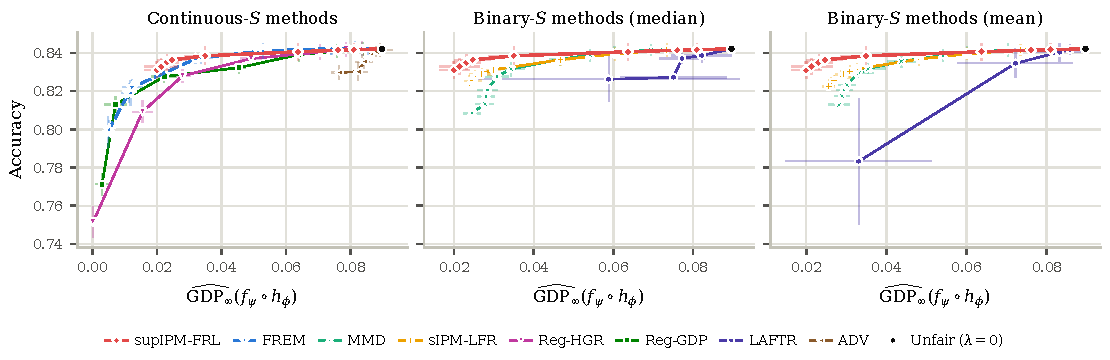
\includegraphics[width=0.76\textwidth]{appendix/fig2_own_head_adult.pdf}\\[1pt]
  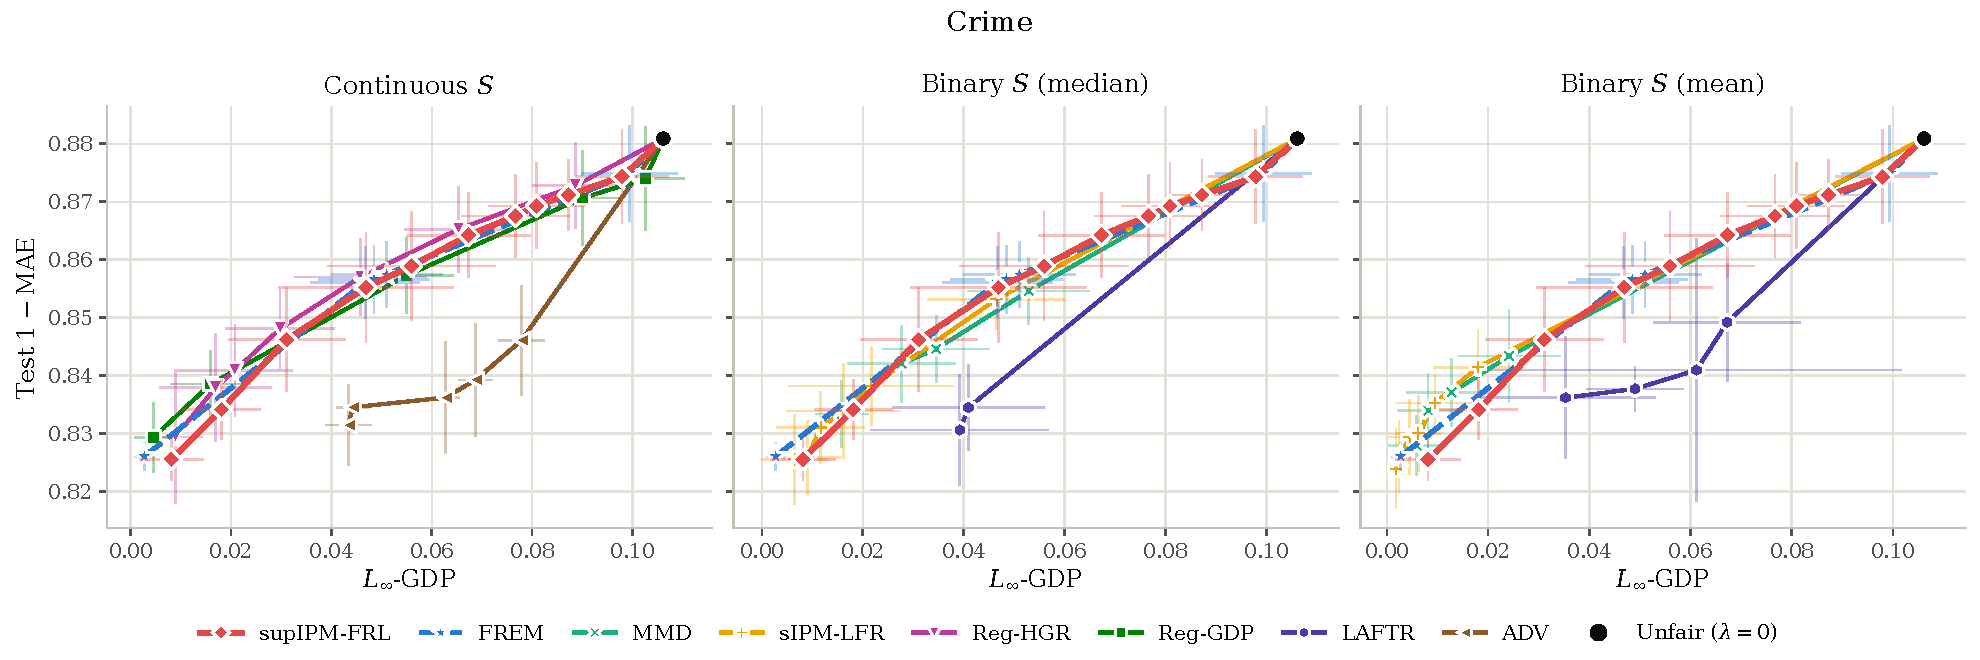
\includegraphics[width=0.76\textwidth]{appendix/fig2_own_head_crime.pdf}\\[1pt]
  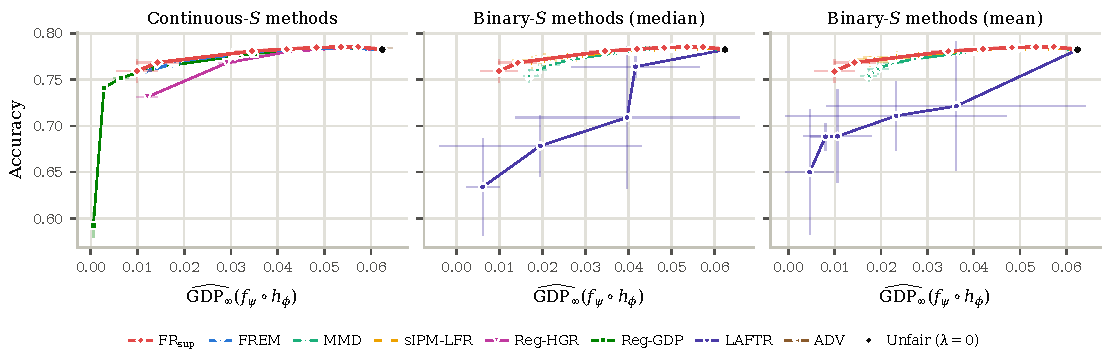
\includegraphics[width=0.76\textwidth]{appendix/fig2_own_head_acs.pdf}
  \caption{Prediction performance against the prediction-level disparity $\widehat{\operatorname{GDP}}_{\infty}(f_{\psi}\circ h_{\phi})$ on Adult (top), Crime (middle) and ACSIncome (bottom).}
  \label{fig:app-prediction-level}
\end{figure}

Figure~\ref{fig:app-c1} repeats the worst-case comparison of Figure~\ref{fig:worst-case} on the three datasets.

\begin{figure}[!htb]
  \centering
  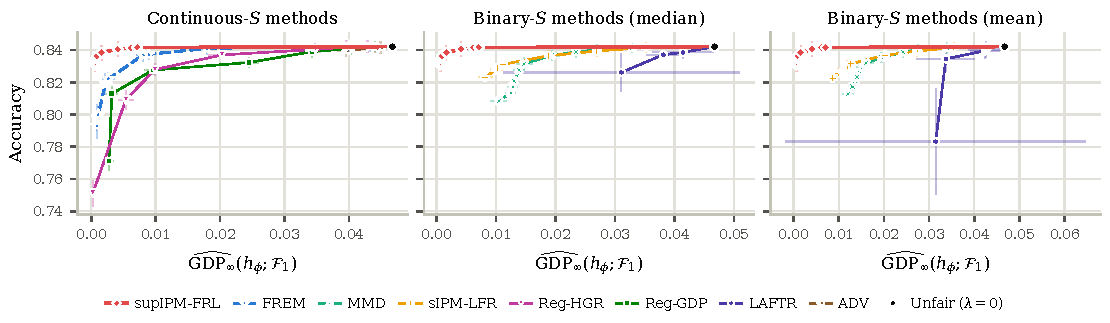
\includegraphics[width=0.76\textwidth]{appendix/figA2_worst_head_budgets_adult_c1.pdf}\\[1pt]
  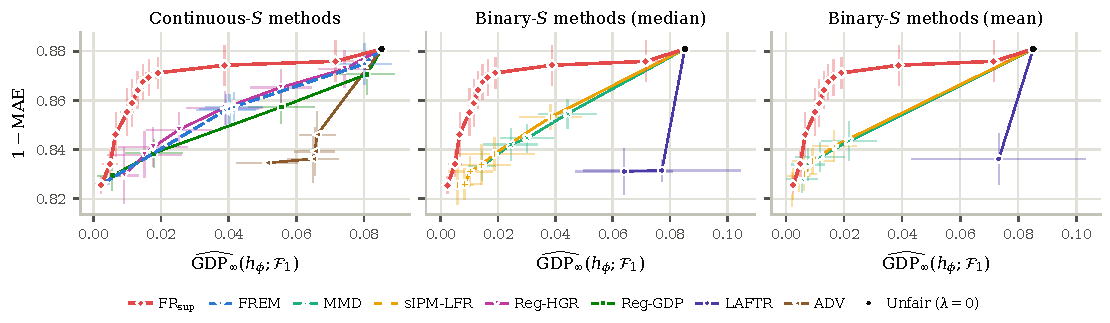
\includegraphics[width=0.76\textwidth]{appendix/figA2_worst_head_budgets_crime_c1.pdf}\\[1pt]
  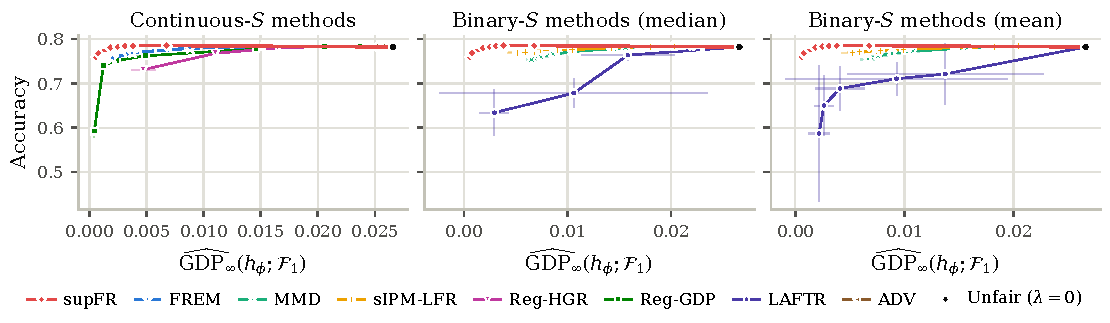
\includegraphics[width=0.76\textwidth]{appendix/figA2_worst_head_budgets_acs_c1.pdf}
  \caption{Prediction performance against the worst-case downstream disparity $\widehat{\operatorname{GDP}}_{\infty}(h_{\phi};\mathcal{F}_{1})$ on Adult (top), Crime (middle) and ACSIncome (bottom).}
  \label{fig:app-c1}
\end{figure}

\paragraph{Other norm bounds.}  Figures~\ref{fig:app-c4} and~\ref{fig:app-c8} repeat the worst-case comparison of Section~\ref{sec:exp-real} with $c=4$ and $c=8$.  The ordering is unchanged, and supIPM-FRL attains the lowest worst-case disparity at a matched level of prediction performance on all three tabular datasets, with Reg-HGR closest to it on Crime at $c=8$, so its advantage persists across the evaluated norm bounds.

\begin{figure}[!htb]
  \centering
  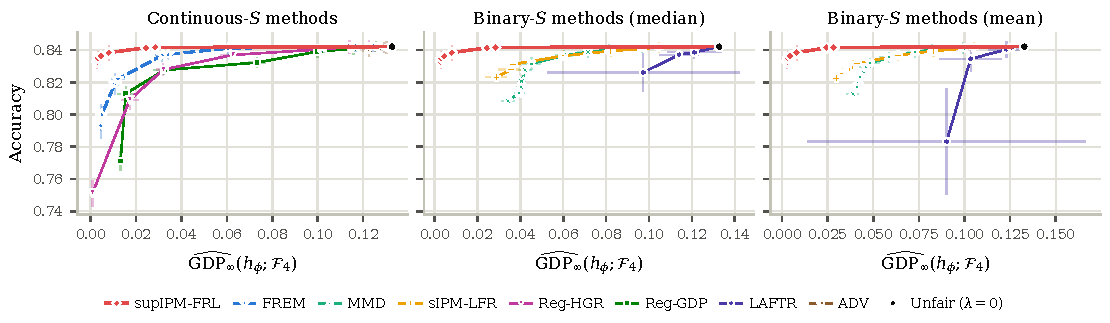
\includegraphics[width=0.76\textwidth]{appendix/figA2_worst_head_budgets_adult_c4.pdf}\\[1pt]
  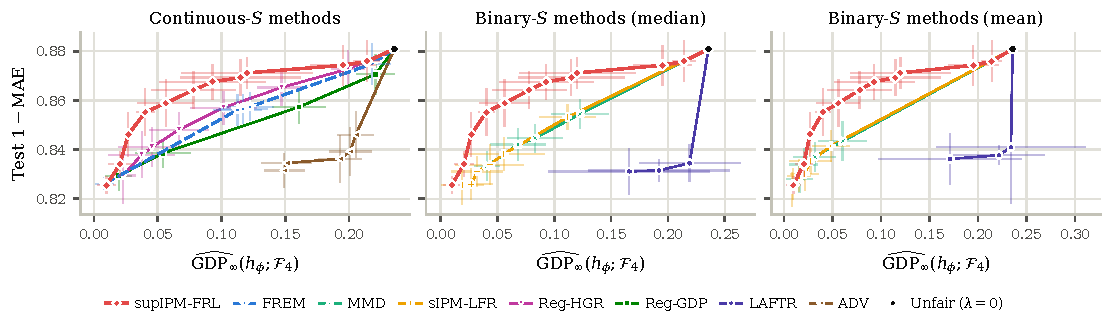
\includegraphics[width=0.76\textwidth]{appendix/figA2_worst_head_budgets_crime_c4.pdf}\\[1pt]
  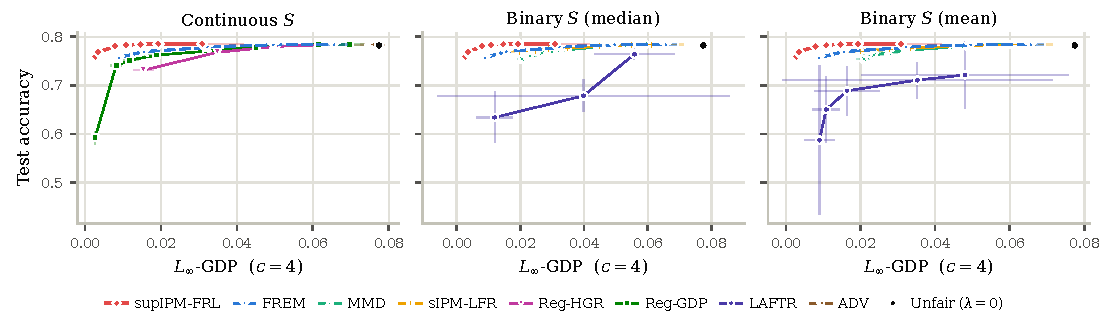
\includegraphics[width=0.76\textwidth]{appendix/figA2_worst_head_budgets_acs_c4.pdf}
  \caption{Prediction performance against the worst-case downstream disparity $\widehat{\operatorname{GDP}}_{\infty}(h_{\phi};\mathcal{F}_{4})$ on Adult (top), Crime (middle) and ACSIncome (bottom).}
  \label{fig:app-c4}
\end{figure}

\begin{figure}[!htb]
  \centering
  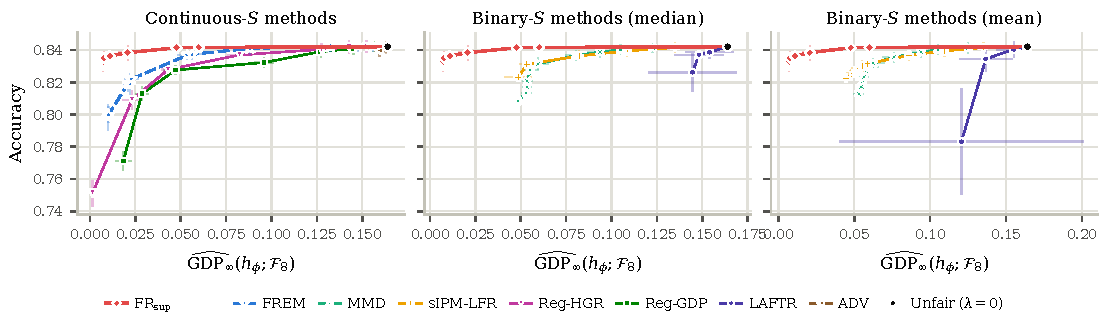
\includegraphics[width=0.76\textwidth]{appendix/figA2_worst_head_budgets_adult_c8.pdf}\\[1pt]
  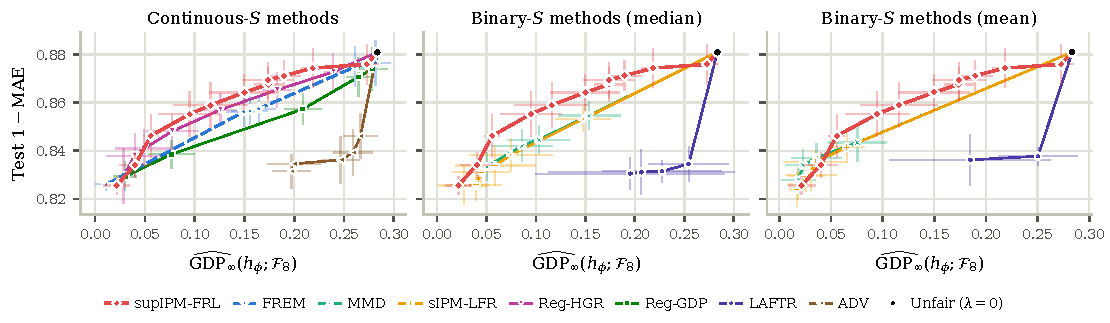
\includegraphics[width=0.76\textwidth]{appendix/figA2_worst_head_budgets_crime_c8.pdf}\\[1pt]
  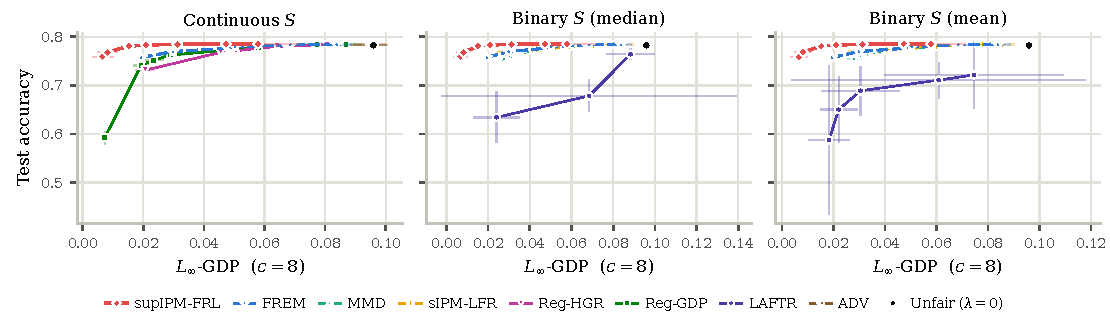
\includegraphics[width=0.76\textwidth]{appendix/figA2_worst_head_budgets_acs_c8.pdf}
  \caption{Prediction performance against the worst-case downstream disparity $\widehat{\operatorname{GDP}}_{\infty}(h_{\phi};\mathcal{F}_{8})$ on Adult (top), Crime (middle) and ACSIncome (bottom).}
  \label{fig:app-c8}
\end{figure}
\FloatBarrier

\paragraph{A larger head class.}  The heads of $\mathcal{F}_c$ are linear in the representation.  Writing
\begin{equation*}
  \mathcal{F}'_c:=\bigl\{\sigma(\mathbf{w}_2^{\top}\operatorname{relu}(\mathbf{W}_1\mathbf{z}+\mathbf{b}_1)+b_2):\ \lVert\mathbf{W}_1\rVert_2\le1,\ \lVert\mathbf{w}_2\rVert_2\le c\bigr\}
\end{equation*}
for the two-layer heads of the same Lipschitz bound, we repeat the comparison over $\mathcal{F}'_1$ in Figure~\ref{fig:app-mlp-head}; the heads are fitted as in Appendix~\ref{app:worst-case} with $16$ hidden units, projecting $\mathbf{W}_1$ onto the spectral-norm ball and $\mathbf{w}_2$ onto the ball of radius $c$ after every step.  Since $\operatorname{relu}(t)-\operatorname{relu}(-t)=t$, two hidden units reproduce any linear head and $\mathcal{F}_c\subset\mathcal{F}'_c$, so the worst case over $\mathcal{F}'_c$ cannot be the smaller of the two.  It is barely the larger: every method's worst-case disparity rises by at most a few percent and the ordering is the one of Section~\ref{sec:exp-real}, so the comparison does not rest on the heads being linear.

\begin{figure}[!htb]
  \centering
  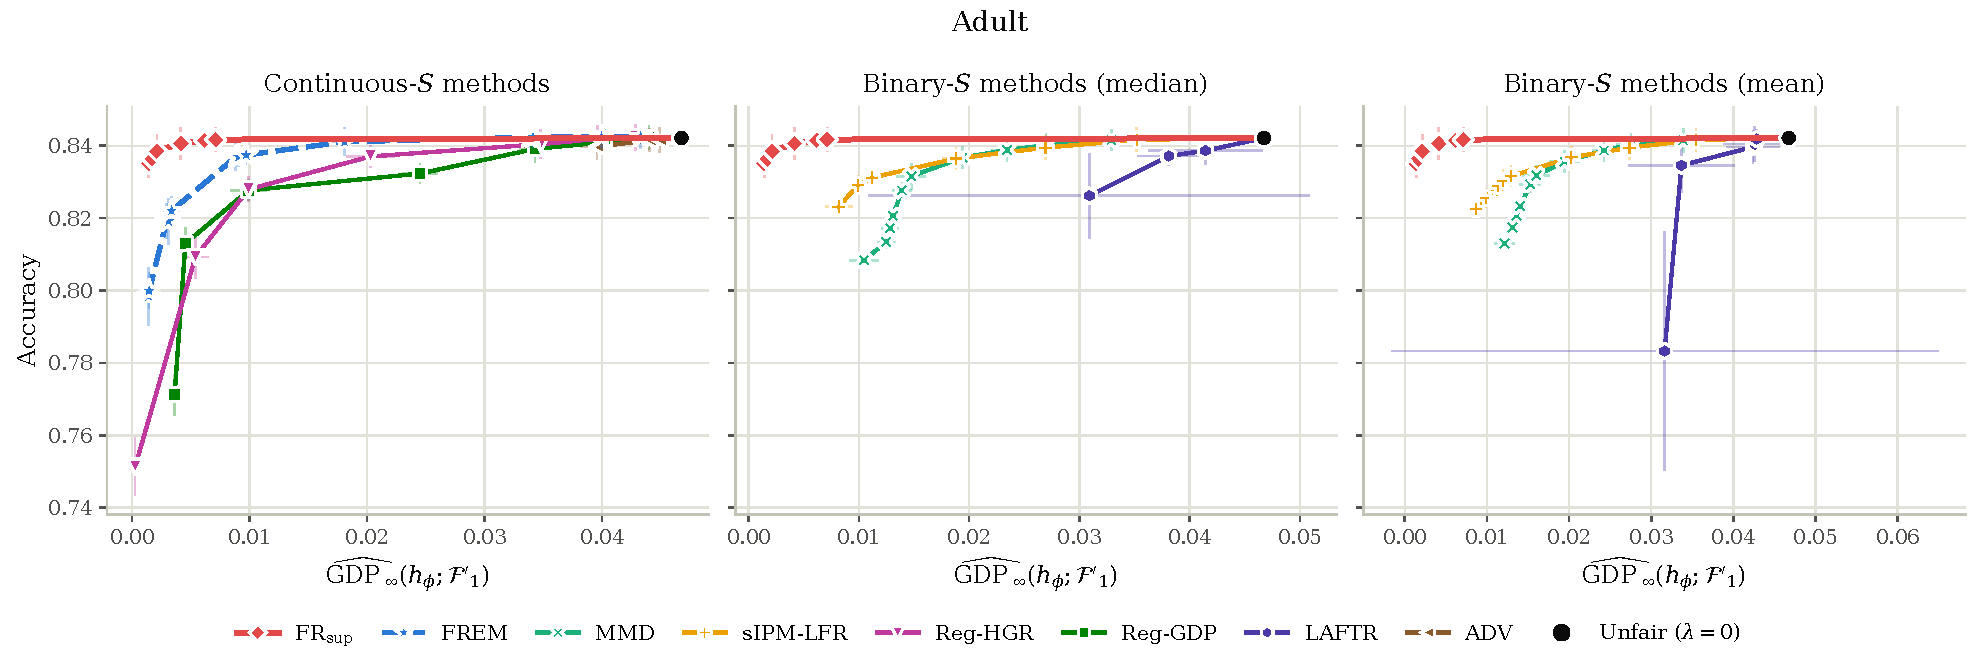
\includegraphics[width=0.8\textwidth]{appendix/figA_worst_head_mlp2_adult.pdf}\\[1pt]
  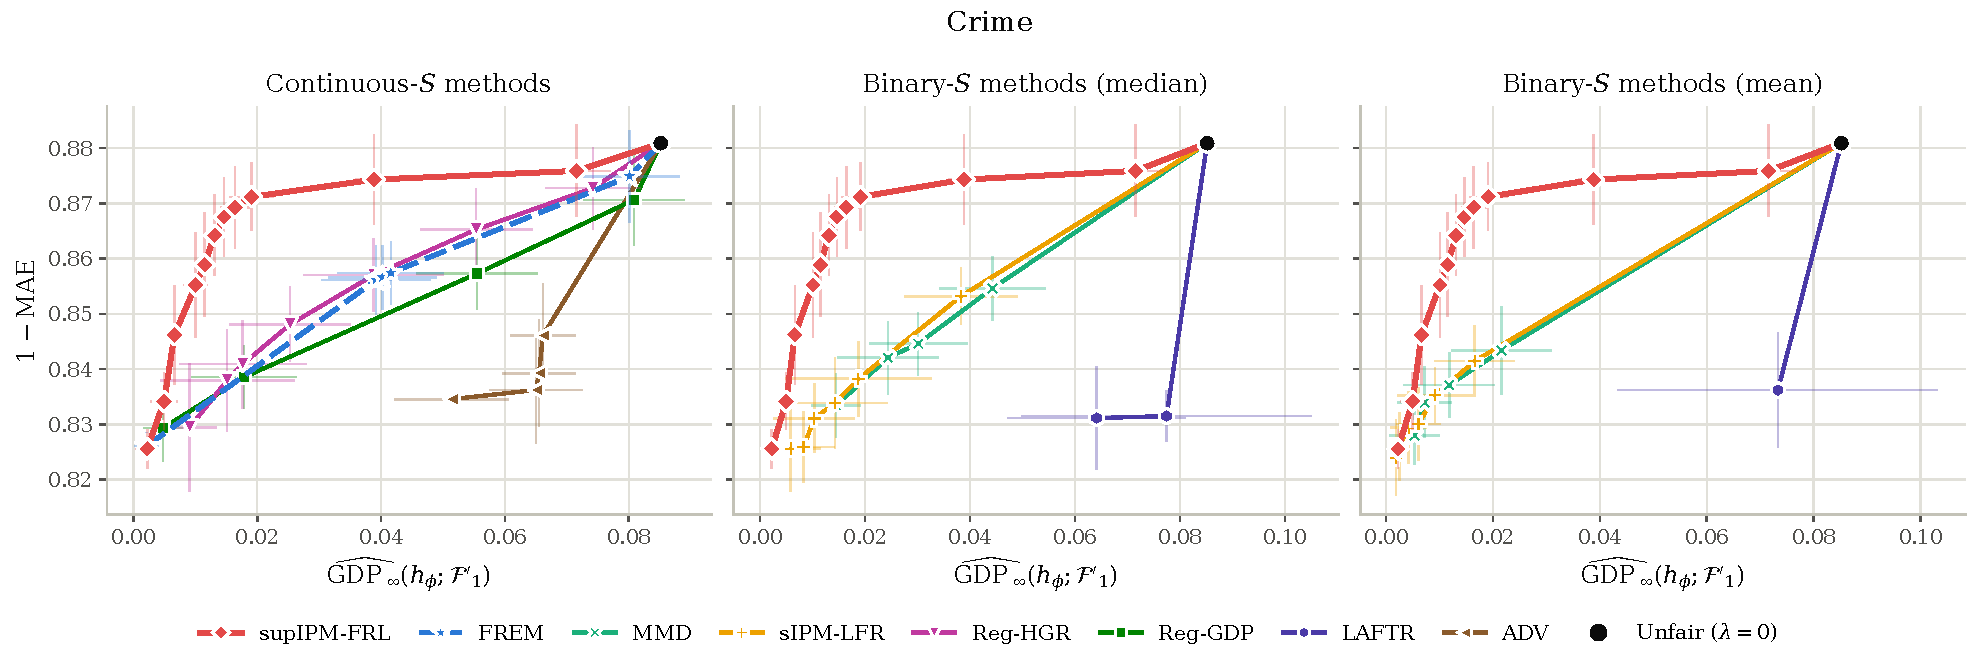
\includegraphics[width=0.8\textwidth]{appendix/figA_worst_head_mlp2_crime.pdf}\\[1pt]
  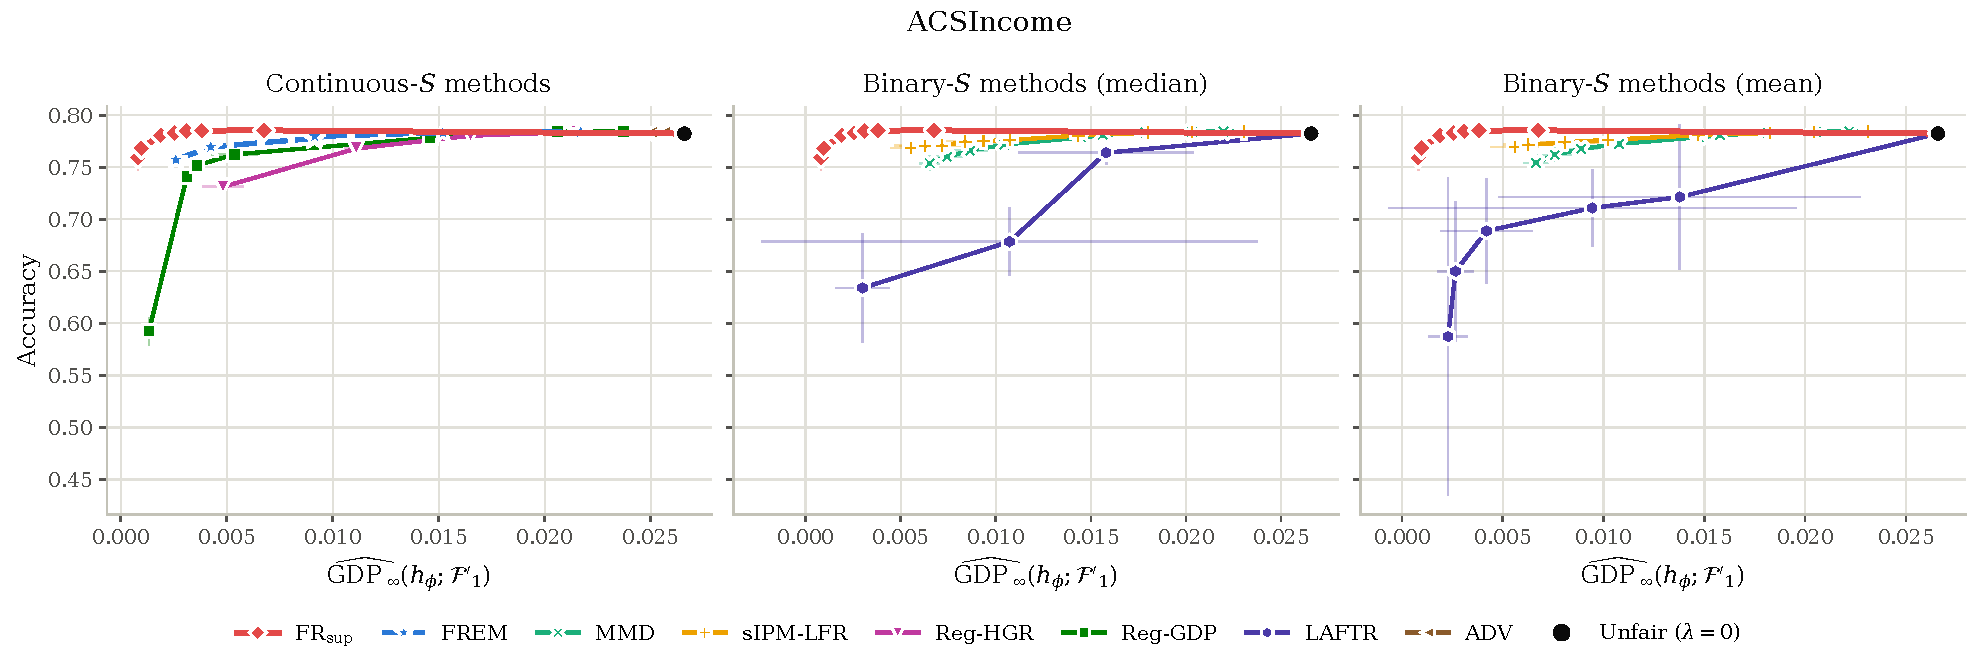
\includegraphics[width=0.8\textwidth]{appendix/figA_worst_head_mlp2_acs.pdf}
  \caption{Prediction performance against the worst-case downstream disparity over the two-layer heads, $\widehat{\operatorname{GDP}}_{\infty}(h_{\phi};\mathcal{F}'_{1})$, on Adult (top), Crime (middle) and ACSIncome (bottom).}
  \label{fig:app-mlp-head}
\end{figure}
\FloatBarrier

\subsubsection{Alternative Fairness Measures}
\label{app:real-measures}

Figures~\ref{fig:app-gdp}--\ref{fig:app-mi-y} replace the disparity axis by the five measures of Appendix~\ref{app:worst-case}.  Under the kernel and the binned estimates of GDP, both averages over $S$, curves of supIPM-FRL and FREM nearly overlap on Adult and Crime and are close on ACSIncome.
% since the average never exceeds the supremum, a bound on the supremum also bounds the average.  
Under the empirical supIPM on the test split, supIPM-FRL is markedly lower than every other method on Adult and Crime, consistent with Theorem~\ref{thm:uniform}.  Under the HGR maximal correlation and the mutual information $I(\hat{Y};S)$, Reg-HGR is lowest and supIPM-FRL is comparable to FREM.

\begin{figure}[!htb]
  \centering
  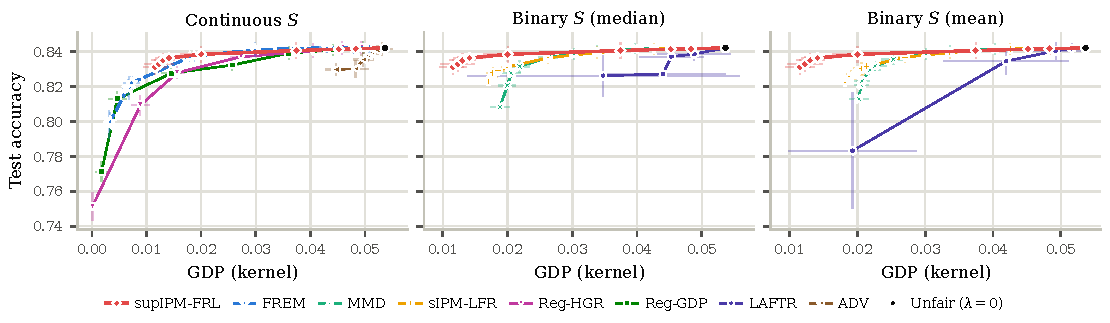
\includegraphics[width=0.76\textwidth]{appendix/figA6_other_measures_adult_gdp_w_kernel.pdf}\\[1pt]
  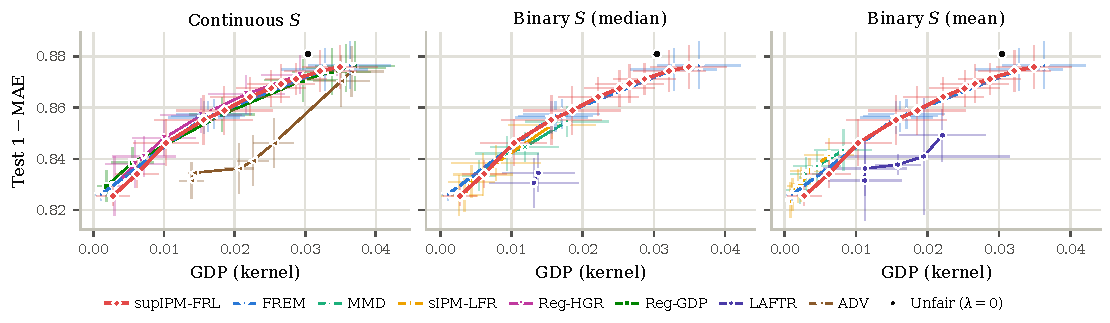
\includegraphics[width=0.76\textwidth]{appendix/figA6_other_measures_crime_gdp_w_kernel.pdf}\\[1pt]
  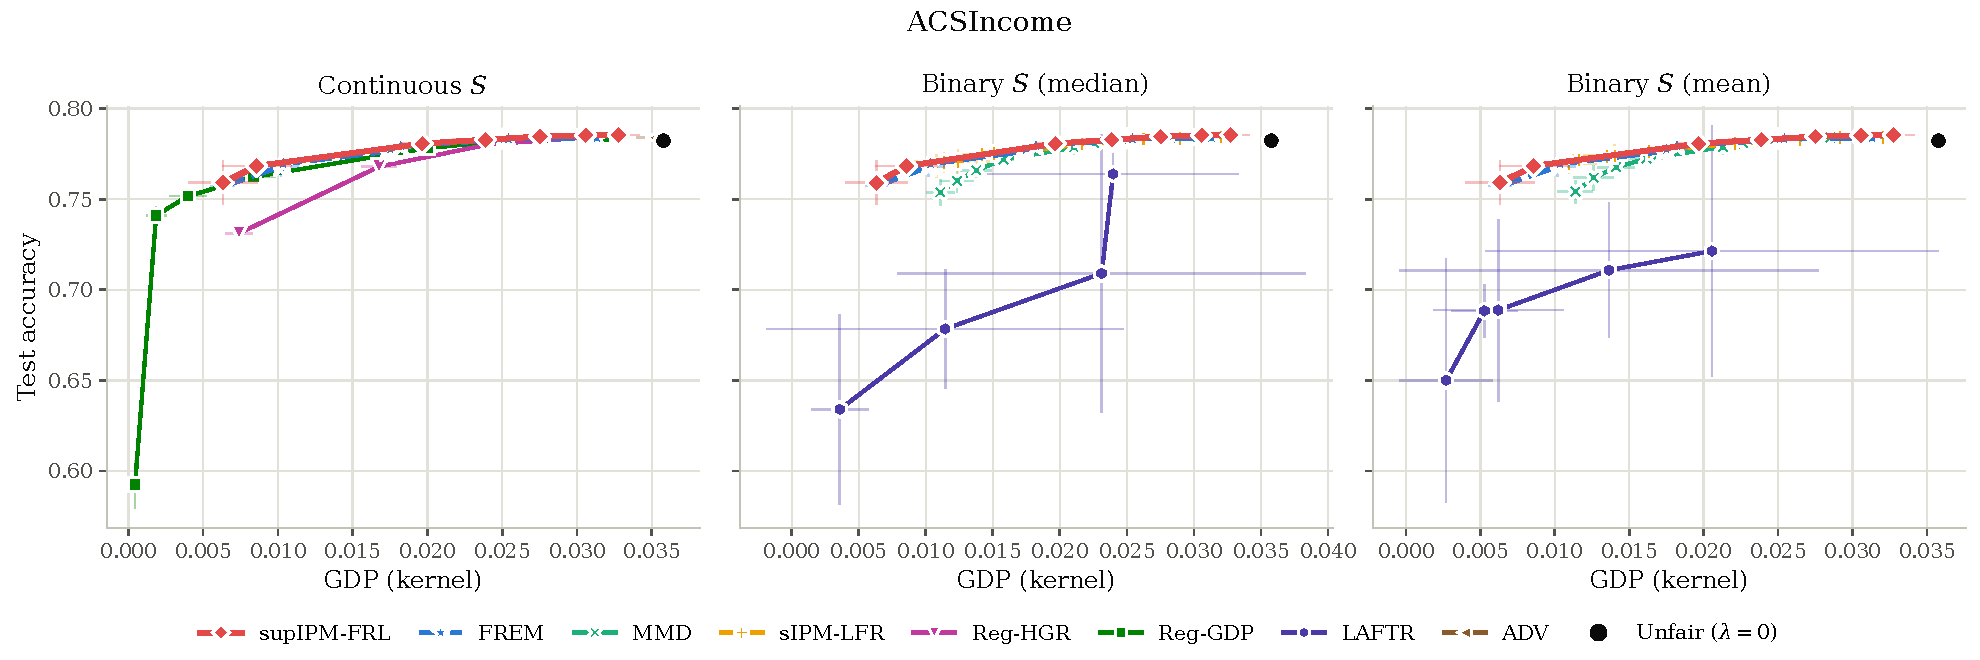
\includegraphics[width=0.76\textwidth]{appendix/figA6_other_measures_acs_gdp_w_kernel.pdf}
  \caption{Prediction performance against the kernel estimate of GDP of the fitted prediction model on Adult (top), Crime (middle) and ACSIncome (bottom).}
  \label{fig:app-gdp}
\end{figure}

\begin{figure}[!htb]
  \centering
  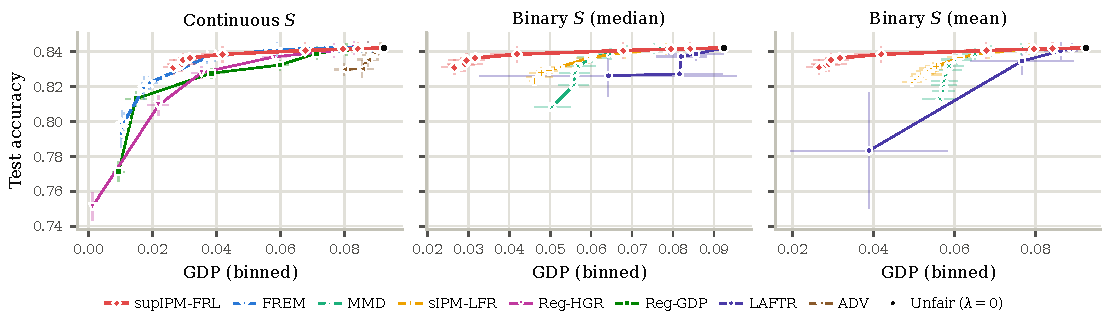
\includegraphics[width=0.76\textwidth]{appendix/figA6_other_measures_adult_gdp_wo_kernel.pdf}\\[1pt]
  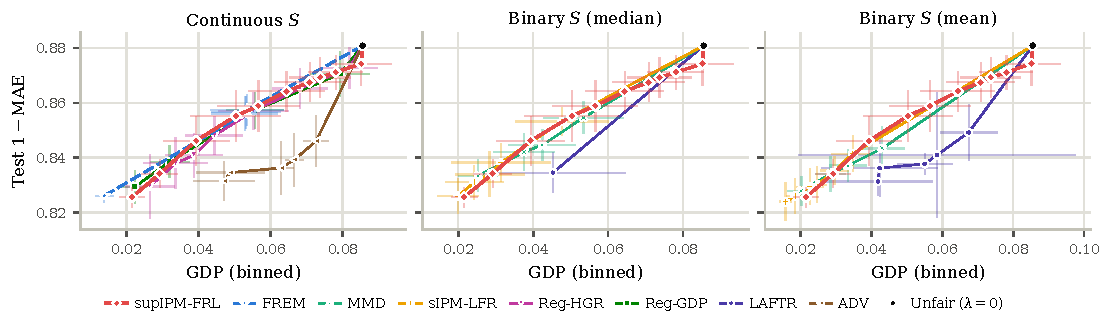
\includegraphics[width=0.76\textwidth]{appendix/figA6_other_measures_crime_gdp_wo_kernel.pdf}\\[1pt]
  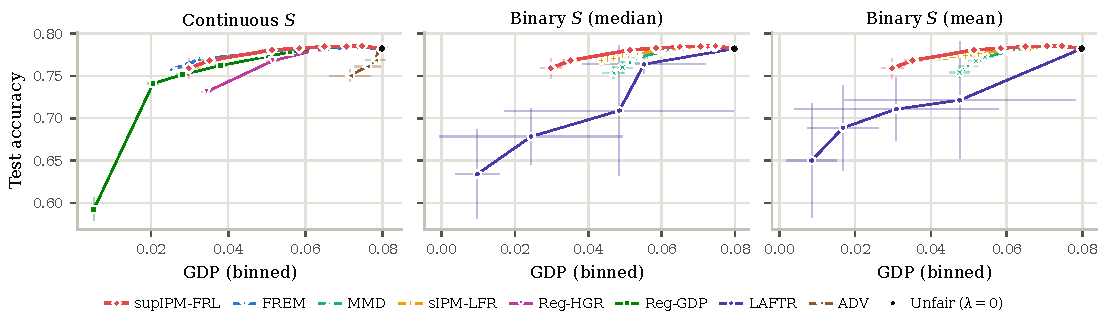
\includegraphics[width=0.76\textwidth]{appendix/figA6_other_measures_acs_gdp_wo_kernel.pdf}
  \caption{Prediction performance against the binned estimate of GDP of the fitted prediction model on Adult (top), Crime (middle) and ACSIncome (bottom).}
  \label{fig:app-gdp-binned}
\end{figure}

\begin{figure}[!htb]
  \centering
  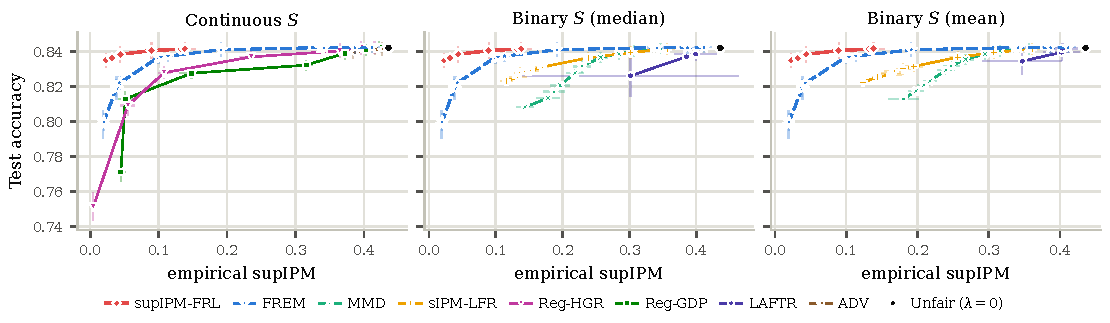
\includegraphics[width=0.76\textwidth]{appendix/figA6_other_measures_adult_sup_ipm.pdf}\\[1pt]
  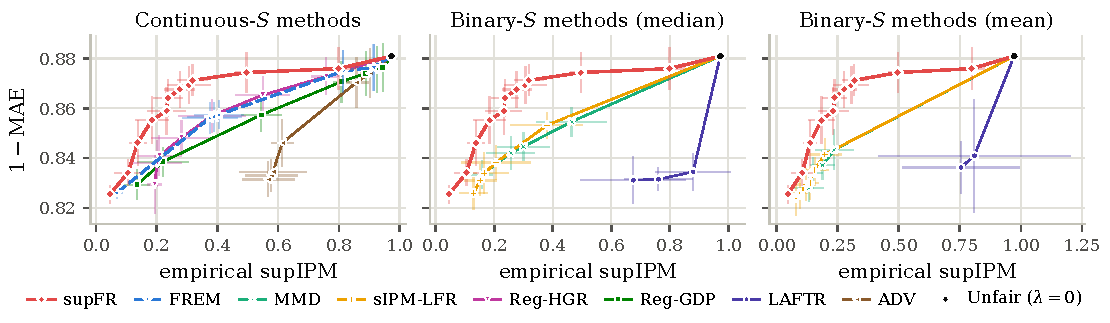
\includegraphics[width=0.76\textwidth]{appendix/figA6_other_measures_crime_sup_ipm.pdf}\\[1pt]
  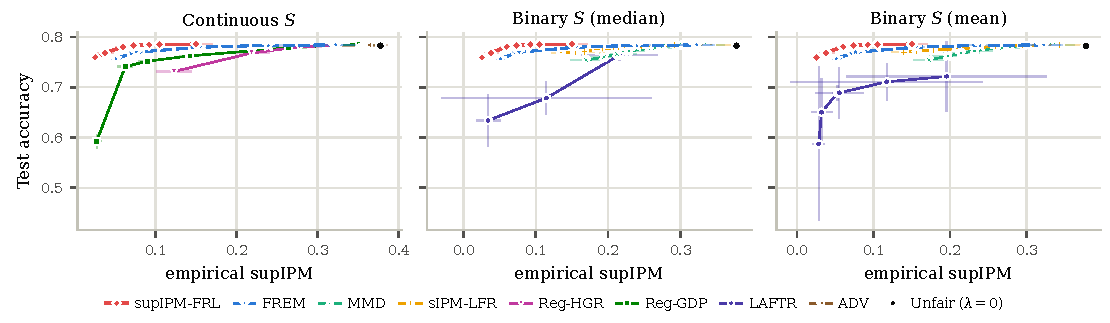
\includegraphics[width=0.76\textwidth]{appendix/figA6_other_measures_acs_sup_ipm.pdf}
  \caption{Prediction performance against the empirical supIPM of the representation on the test split on Adult (top), Crime (middle) and ACSIncome (bottom).}
  \label{fig:app-supipm}
\end{figure}

\begin{figure}[!htb]
  \centering
  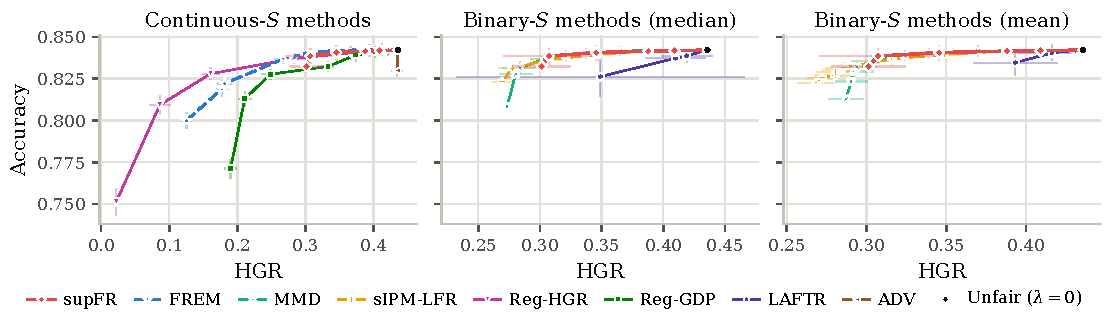
\includegraphics[width=0.76\textwidth]{appendix/figA6_other_measures_adult_hgr.pdf}\\[1pt]
  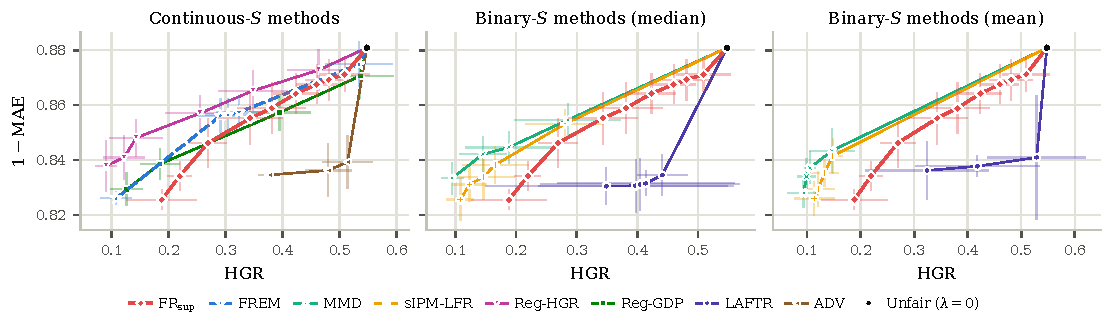
\includegraphics[width=0.76\textwidth]{appendix/figA6_other_measures_crime_hgr.pdf}\\[1pt]
  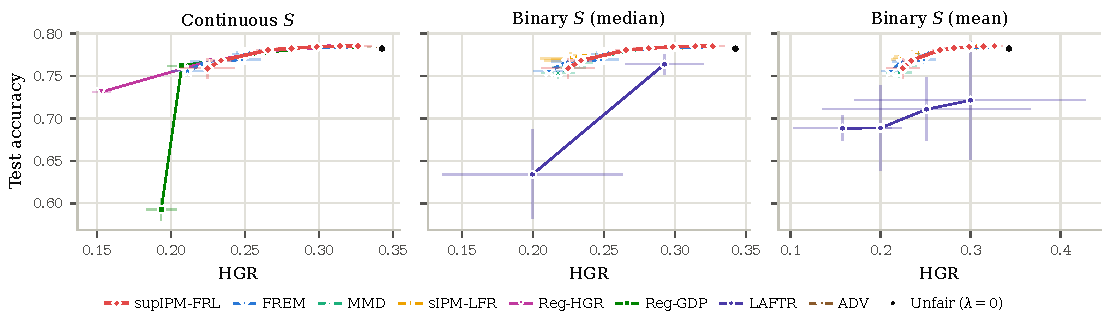
\includegraphics[width=0.76\textwidth]{appendix/figA6_other_measures_acs_hgr.pdf}
  \caption{Prediction performance against the HGR maximal correlation between the fitted prediction and $S$ on Adult (top), Crime (middle) and ACSIncome (bottom).}
  \label{fig:app-hgr}
\end{figure}

\begin{figure}[!htb]
  \centering
  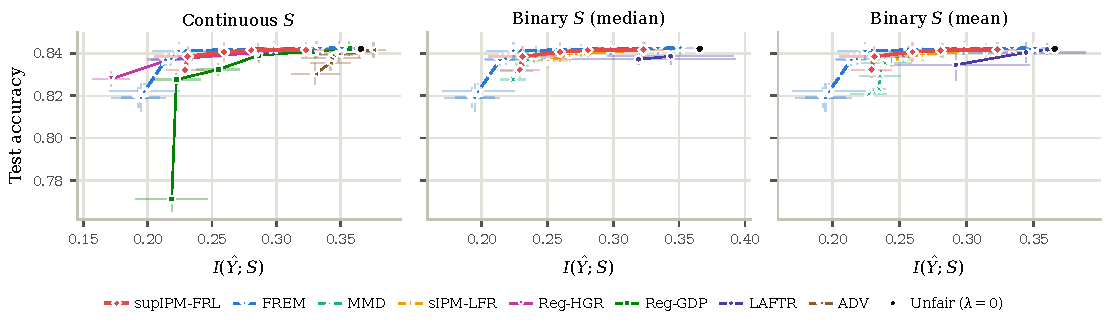
\includegraphics[width=0.76\textwidth]{appendix/figA6_other_measures_adult_mi_y_s.pdf}\\[1pt]
  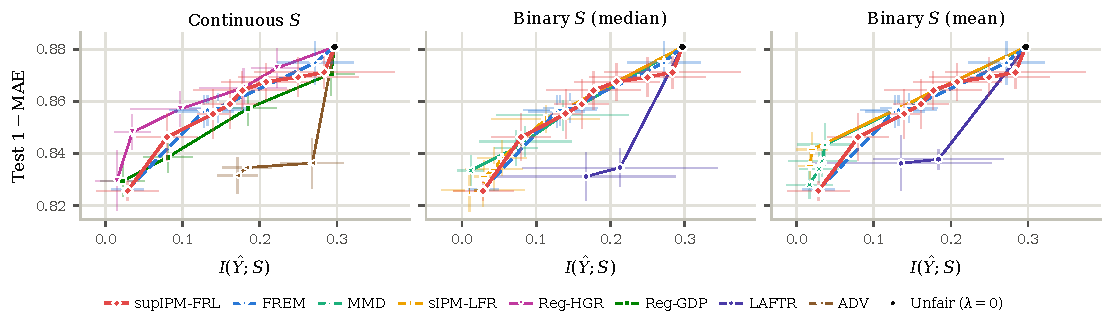
\includegraphics[width=0.76\textwidth]{appendix/figA6_other_measures_crime_mi_y_s.pdf}\\[1pt]
  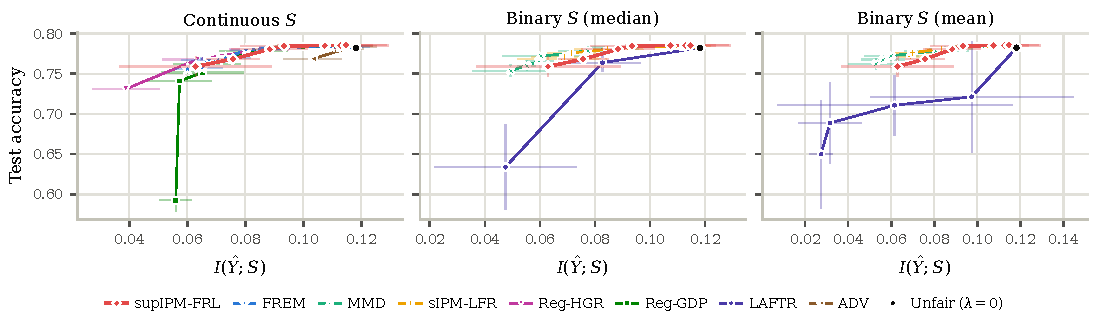
\includegraphics[width=0.76\textwidth]{appendix/figA6_other_measures_acs_mi_y_s.pdf}
  \caption{Prediction performance against the mutual information $I(\hat{Y};S)$ between the fitted prediction and $S$ on Adult (top), Crime (middle) and ACSIncome (bottom).}
  \label{fig:app-mi-y}
\end{figure}
\FloatBarrier

\subsubsection{Graph Datasets}
\label{app:real-graph}

For the graph experiments,  we compare supIPM-FRL with FREM, Reg-GDP, Reg-HGR, ADV, and MMD. LAFTR and sIPM-LFR are evaluated only on the tabular datasets.  
On Pokec-z and Pokec-n (Figure~\ref{fig:app-graph}), supIPM-FRL, FREM and Reg-GDP have similar prediction-level curves.  Under the worst-case disparity, supIPM-FRL and FREM coincide, MMD is close to them, and Reg-GDP and Reg-HGR attain larger disparities.  On these graphs the supremum and the average penalty control the downstream heads equally well, whereas a penalty on the fitted head does not.

\begin{figure}[!htb]
  \centering
  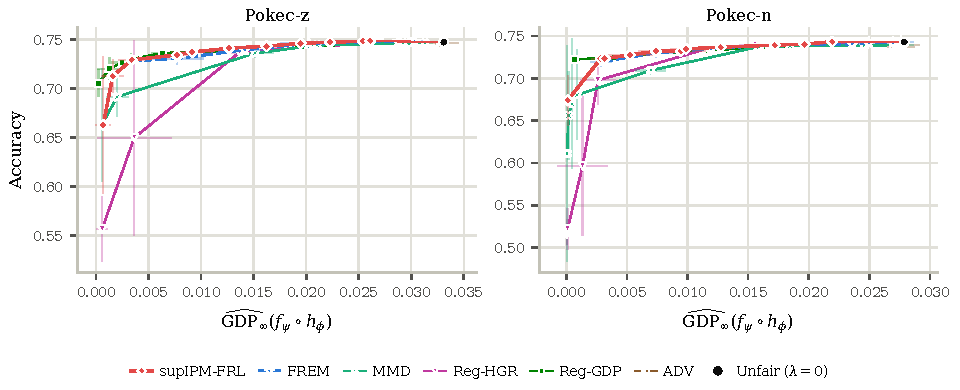
\includegraphics[width=0.68\textwidth]{appendix/figA7_graph_own_head.pdf}\\[1pt]
  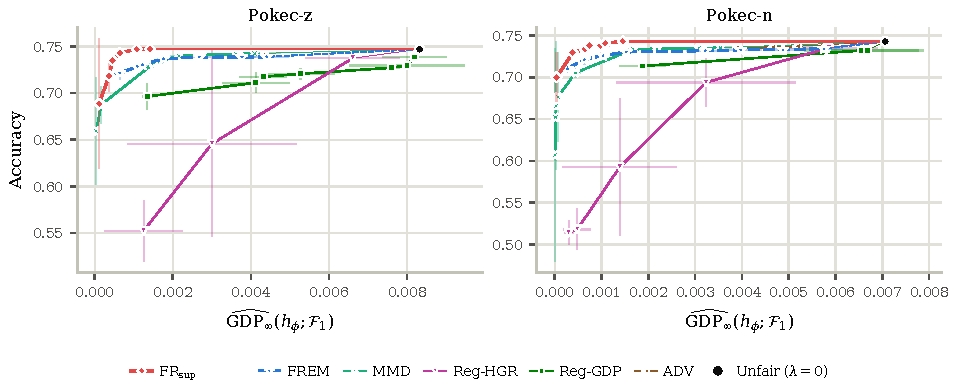
\includegraphics[width=0.68\textwidth]{appendix/figA7_graph_worst_head.pdf}
  \caption{Pokec-z (left) and Pokec-n (right): prediction performance against the prediction-level disparity $\widehat{\operatorname{GDP}}_{\infty}(f_{\psi}\circ h_{\phi})$ (top) and the worst-case downstream disparity $\widehat{\operatorname{GDP}}_{\infty}(h_{\phi};\mathcal{F}_1)$ (bottom).}
  \label{fig:app-graph}
\end{figure}

Figures~\ref{fig:app-graph-gdp-kernel}--\ref{fig:app-graph-mi} replace the disparity axis by the other measures of Appendix~\ref{app:worst-case}, as in Appendix~\ref{app:real-measures}.

\begin{figure}[!htb]
  \centering
  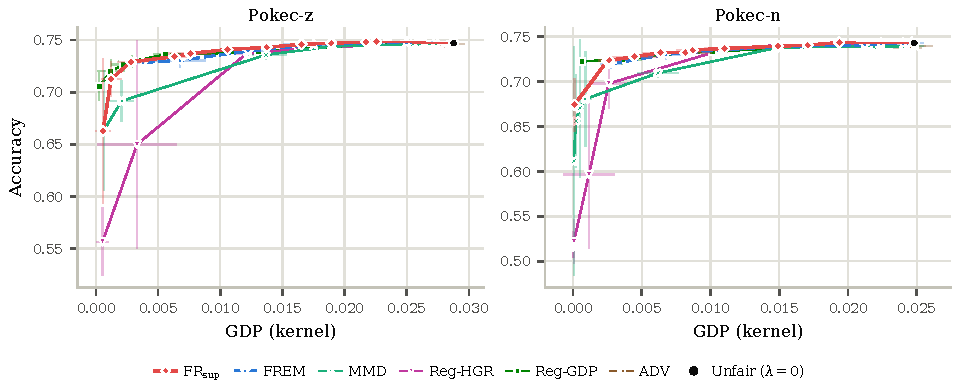
\includegraphics[width=0.68\textwidth]{appendix/figA7_graph_gdp_w_kernel.pdf}\\[1pt]
  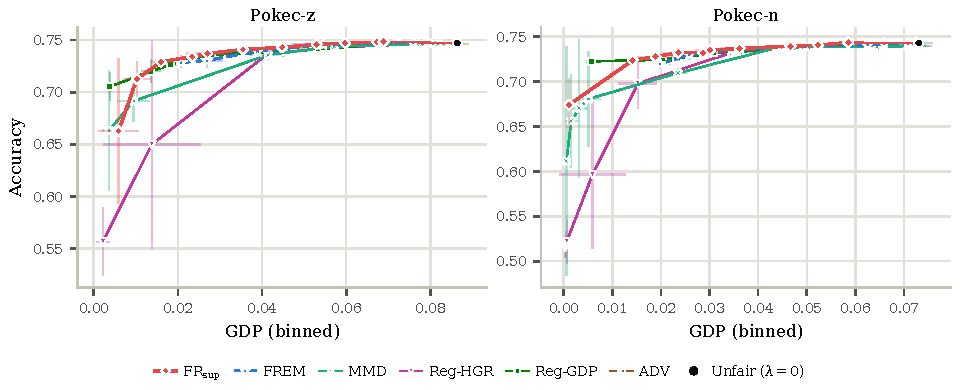
\includegraphics[width=0.68\textwidth]{appendix/figA7_graph_gdp_wo_kernel.pdf}\\[1pt]
  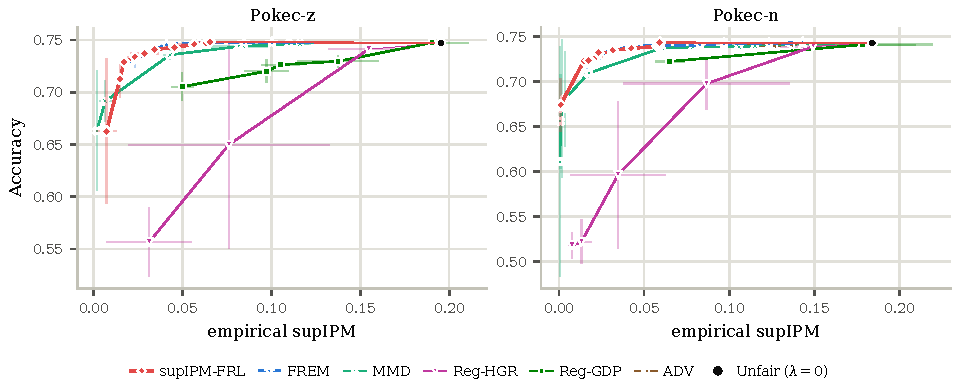
\includegraphics[width=0.68\textwidth]{appendix/figA7_graph_sup_ipm.pdf}
  \caption{Pokec-z (left) and Pokec-n (right): prediction performance against the kernel GDP (top), the binned GDP (middle) and the empirical supIPM (bottom).}
  \label{fig:app-graph-gdp-kernel}
\end{figure}

\begin{figure}[!htb]
  \centering
  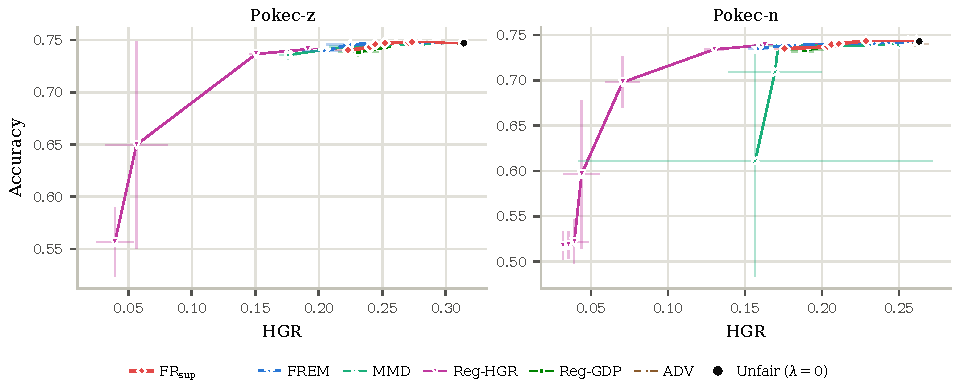
\includegraphics[width=0.68\textwidth]{appendix/figA7_graph_hgr.pdf}\\[1pt]
  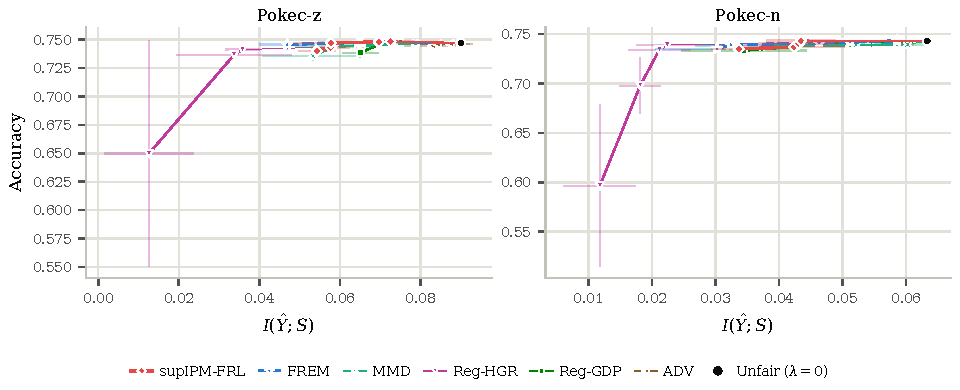
\includegraphics[width=0.68\textwidth]{appendix/figA7_graph_mi_y_s.pdf}
  \caption{Pokec-z (left) and Pokec-n (right): prediction performance against the HGR maximal correlation (top) and the mutual information $I(\hat{Y};S)$ (bottom).}
  \label{fig:app-graph-mi}
\end{figure}

\FloatBarrier

\subsubsection{Matched-Performance Comparison}
\label{app:real-matched}

Table~\ref{tab:matched} compares the methods at similar levels of prediction performance. supIPM-FRL achieves the lowest prediction-level and worst-case disparity in every case except the prediction-level disparity on Crime, where it remains comparable to the smallest value. In particular, supIPM-FRL substantially outperforms all baselines in the worst-case downstream disparity on all three datasets. Each dataset is compared at the prediction performance shown in the table, up to a margin of $0.004$.  An entry is the smallest disparity the method attains there.  A dash means that the method did not reach that performance.  The best value in each row is in bold.

\begin{table}[!htb]
\centering
\caption{Comparison of algorithms in terms of $\widehat{\operatorname{GDP}}_{\infty}(f_{\psi}\circ h_{\phi})$ and $\widehat{\operatorname{GDP}}_{\infty}(h_{\phi};\mathcal{F}_1)$.}
\label{tab:matched}
\footnotesize
\setlength{\tabcolsep}{3pt}
\begin{tabular}{lrrrrrrrr}
\toprule
 & supIPM-FRL & FREM & Reg-GDP & Reg-HGR & ADV & LAFTR & MMD & sIPM-LFR \\
\midrule
\multicolumn{9}{l}{\emph{Adult, accuracy $0.842$}} \\
prediction-level & $\mathbf{0.0350}$ & 0.0529 & 0.0639 & 0.0706 & 0.0855 & 0.0822 & 0.0541 & 0.0601 \\
worst-case ($c=1$) & $\mathbf{0.0014}$ & 0.0086 & 0.0339 & 0.0192 & 0.0388 & 0.0403 & 0.0186 & 0.0197 \\
\midrule
\multicolumn{9}{l}{\emph{Crime, $1-\mathrm{MAE}$ $0.855$}} \\
prediction-level & 0.0469 & 0.0468 & 0.0550 & $\mathbf{0.0458}$ & -- & -- & 0.0529 & 0.0465 \\
worst-case ($c=1$) & $\mathbf{0.0100}$ & 0.0338 & 0.0504 & 0.0315 & -- & -- & 0.0380 & 0.0314 \\
\midrule
\multicolumn{9}{l}{\emph{ACSIncome, accuracy $0.780$}} \\
prediction-level & $\mathbf{0.0279}$ & 0.0302 & 0.0350 & 0.0423 & 0.0617 & -- & 0.0368 & 0.0281 \\
worst-case ($c=1$) & $\mathbf{0.0018}$ & 0.0088 & 0.0146 & 0.0165 & 0.0248 & -- & 0.0145 & 0.0099 \\
\bottomrule
\end{tabular}
\end{table}
\FloatBarrier

\subsection{Computational Cost}
\label{app:real-cost}

Appendix~\ref{app:mini-batch} shows that supIPM-FRL admits mini-batch learning with unbiased gradients.  No such formulation is available for the MMD penalty of FREM \citep{lee2026fair}, so FREM is trained on the batch, that is, on the whole training sample.  Table~\ref{tab:cost} reports one gradient step on Adult for mini-batch and for batch learning, and includes sup-MMD, the variant of Appendix~\ref{app:ablation-ipm-class} with the MMD in place of the ReLU discriminators.

\begin{table}[H]
\centering
\footnotesize
\caption{One gradient step on Adult.}
\label{tab:cost}
\begin{tabular}{llrr}
\toprule
Method & learning & seconds & peak memory (MB) \\
\midrule
supIPM-FRL & mini-batch ($1{,}024$) & 0.086 & 33 \\
FREM       & batch ($32{,}000$) & \multicolumn{2}{c}{out of memory} \\
sup-MMD    & batch ($32{,}000$) & \multicolumn{2}{c}{out of memory} \\
\bottomrule
\end{tabular}
\end{table}

The MMD evaluates the kernel at every pair of representations, so its cost grows quadratically with the number of observations.  On the whole batch, this cost exceeds the $24$ GB of the GPU.  In practice, FREM and sup-MMD are therefore trained with mini-batches, whose gradients are biased for the batch objective.  Figure~\ref{fig:cost} gives the computational cost as the mini-batch grows.  FREM already needs $8.5$ GB at $1{,}024$ observations.  The memory of supIPM-FRL grows linearly and the whole training sample takes $129$ MB, while its time per step is almost the same as with the mini-batch.

\begin{figure}[H]
  \centering
  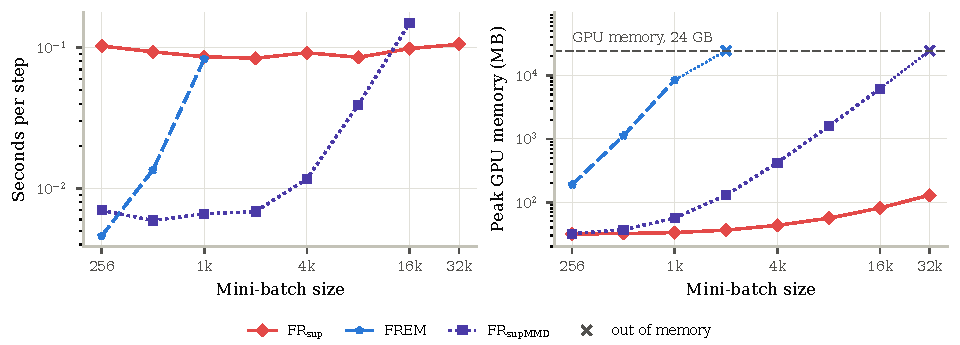
\includegraphics[width=0.92\textwidth]{appendix/figAC_cost.pdf}
  \caption{One gradient step on Adult as the mini-batch grows.  The cross marks the first size that exceeds the memory of the GPU.}
  \label{fig:cost}
\end{figure}

The linear cost of supIPM-FRL, together with the unbiased mini-batch gradients of Appendix~\ref{app:mini-batch}, is the main reason for the ReLU discriminators of Section~\ref{sec:discriminator-choice}.

\section{Ablation Studies}
\label{app:ablation-studies}

This appendix examines two choices in the penalty of supIPM-FRL on the tabular datasets: the shape of the smoothing kernel and the class of the discriminators.  Each ablation varies one choice and holds every other setting of Appendix~\ref{app:real-settings} fixed.  Each figure reports prediction performance against the prediction-level disparity in the top row and against the worst-case downstream disparity over $\mathcal{F}_1$ in the bottom row, with one column per dataset.

% The bandwidth ablation is commented out for now.
% \subsection{Bandwidth}
% \label{app:ablation-bandwidth}
%
% The bandwidth $\gamma$ of the kernel $K_{\gamma}$ in Equation~(\ref{eq:supipm-estimators}) sets the range of sensitive values over which the conditional distribution at $s$ is smoothed.  We train supIPM-FRL at $\gamma\in\{0.10,0.25,0.50\}\,\widehat{\sigma}_S$ in place of the bandwidth of Appendix~\ref{app:synth-settings}, and leave the evaluation smoother unchanged.
%
% In Figure~\ref{fig:app-ablation-bandwidth} the prediction-level curves nearly coincide.  At a matched level of prediction performance $\gamma=0.25$ attains a lower worst-case disparity than $\gamma=0.50$ on the three datasets and than $\gamma=0.10$ on Crime and ACSIncome, while on Adult the narrower bandwidth is the lower of the two.
%
% \begin{figure}[!htb]
%   \centering
%   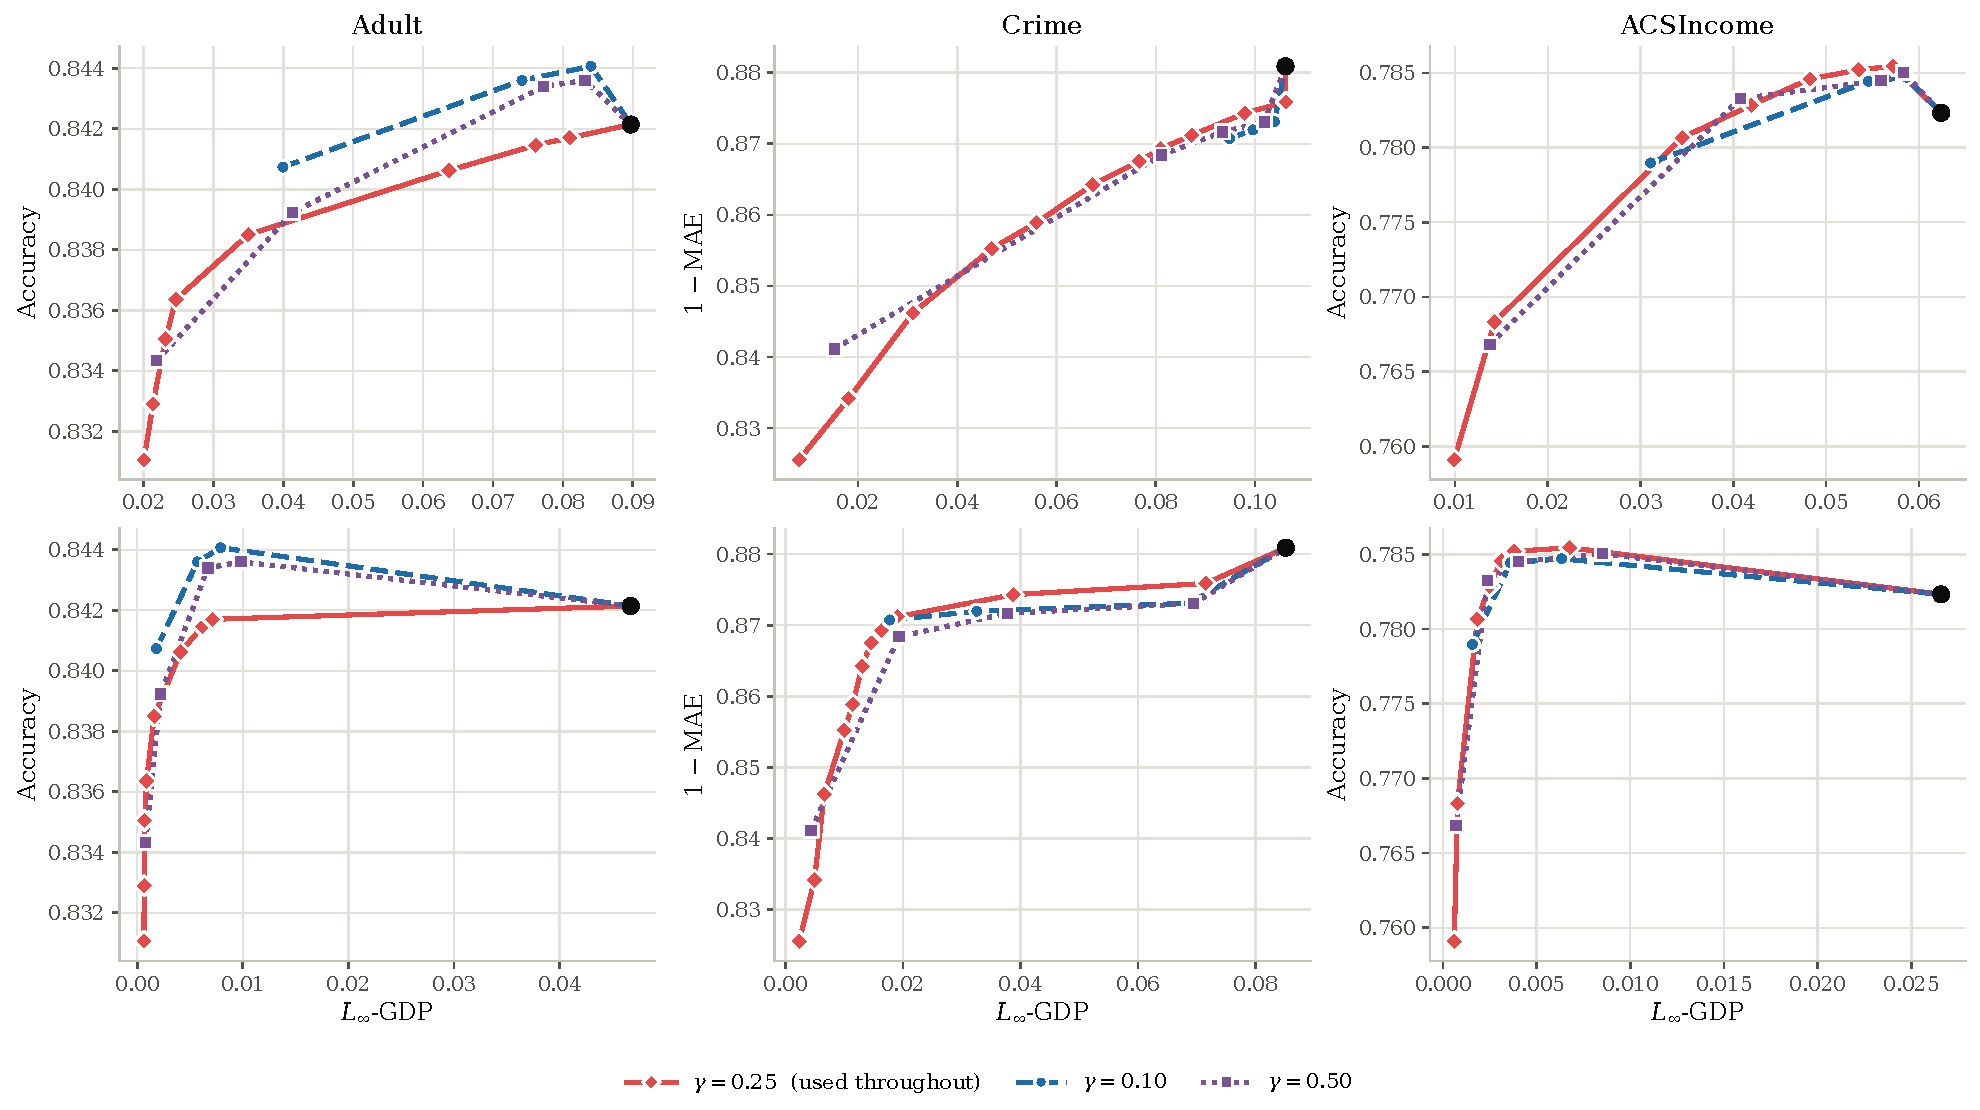
\includegraphics[width=\textwidth]{appendix/figAB_bandwidth.pdf}
%   \caption{Prediction performance against the prediction-level disparity $\widehat{\operatorname{GDP}}_{\infty}(f_{\psi}\circ h_{\phi})$ (top) and the worst-case downstream disparity $\widehat{\operatorname{GDP}}_{\infty}(h_{\phi};\mathcal{F}_{1})$ (bottom) for supIPM-FRL trained at $\gamma\in\{0.10,0.25,0.50\}$, on Adult (left), Crime (middle) and ACSIncome (right).}
%   \label{fig:app-ablation-bandwidth}
% \end{figure}
% \FloatBarrier

\subsection{Smoothing Kernel}
\label{app:ablation-kernel}

The shape of $K_{\gamma}$ determines how the sensitive values neighboring $s$ are weighted.  Writing $u$ for the distance between two sensitive values in units of the bandwidth, we compare four shapes.
\begin{itemize}[leftmargin=*, itemsep=0pt, topsep=2pt]
  \item Gaussian:
    \begin{equation*} K(u)\propto\exp(-u^{2}/2). \end{equation*}
  \item Epanechnikov:
    \begin{equation*} K(u)\propto(1-u^{2})_{+}. \end{equation*}
  \item Triangular:
    \begin{equation*} K(u)\propto(1-|u|)_{+}. \end{equation*}
  \item Box:
    \begin{equation*} K(u)\propto\mathbf{1}\{|u|\le1\}. \end{equation*}
\end{itemize}
The last three vanish beyond a fixed distance from $s$, and the four are scaled to the same second moment, so that the comparison isolates the shape from the spread.

In Figure~\ref{fig:app-ablation-kernel} no kernel is uniformly best at a matched level of prediction performance: the lowest worst-case disparity is attained by the Gaussian on Crime, by the box kernel on ACSIncome and by the compactly supported kernels on Adult, each within a factor of $1.4$ of the Gaussian.  The kernels differ instead in the penalty values they admit.  
With a compactly supported kernel the representation collapses to a constant predictor at a smaller $\lambda$, so the curves of the compactly supported kernels stop at a disparity that the Gaussian kernel still reaches with a nonconstant predictor.

\begin{figure}[!htb]
  \centering
  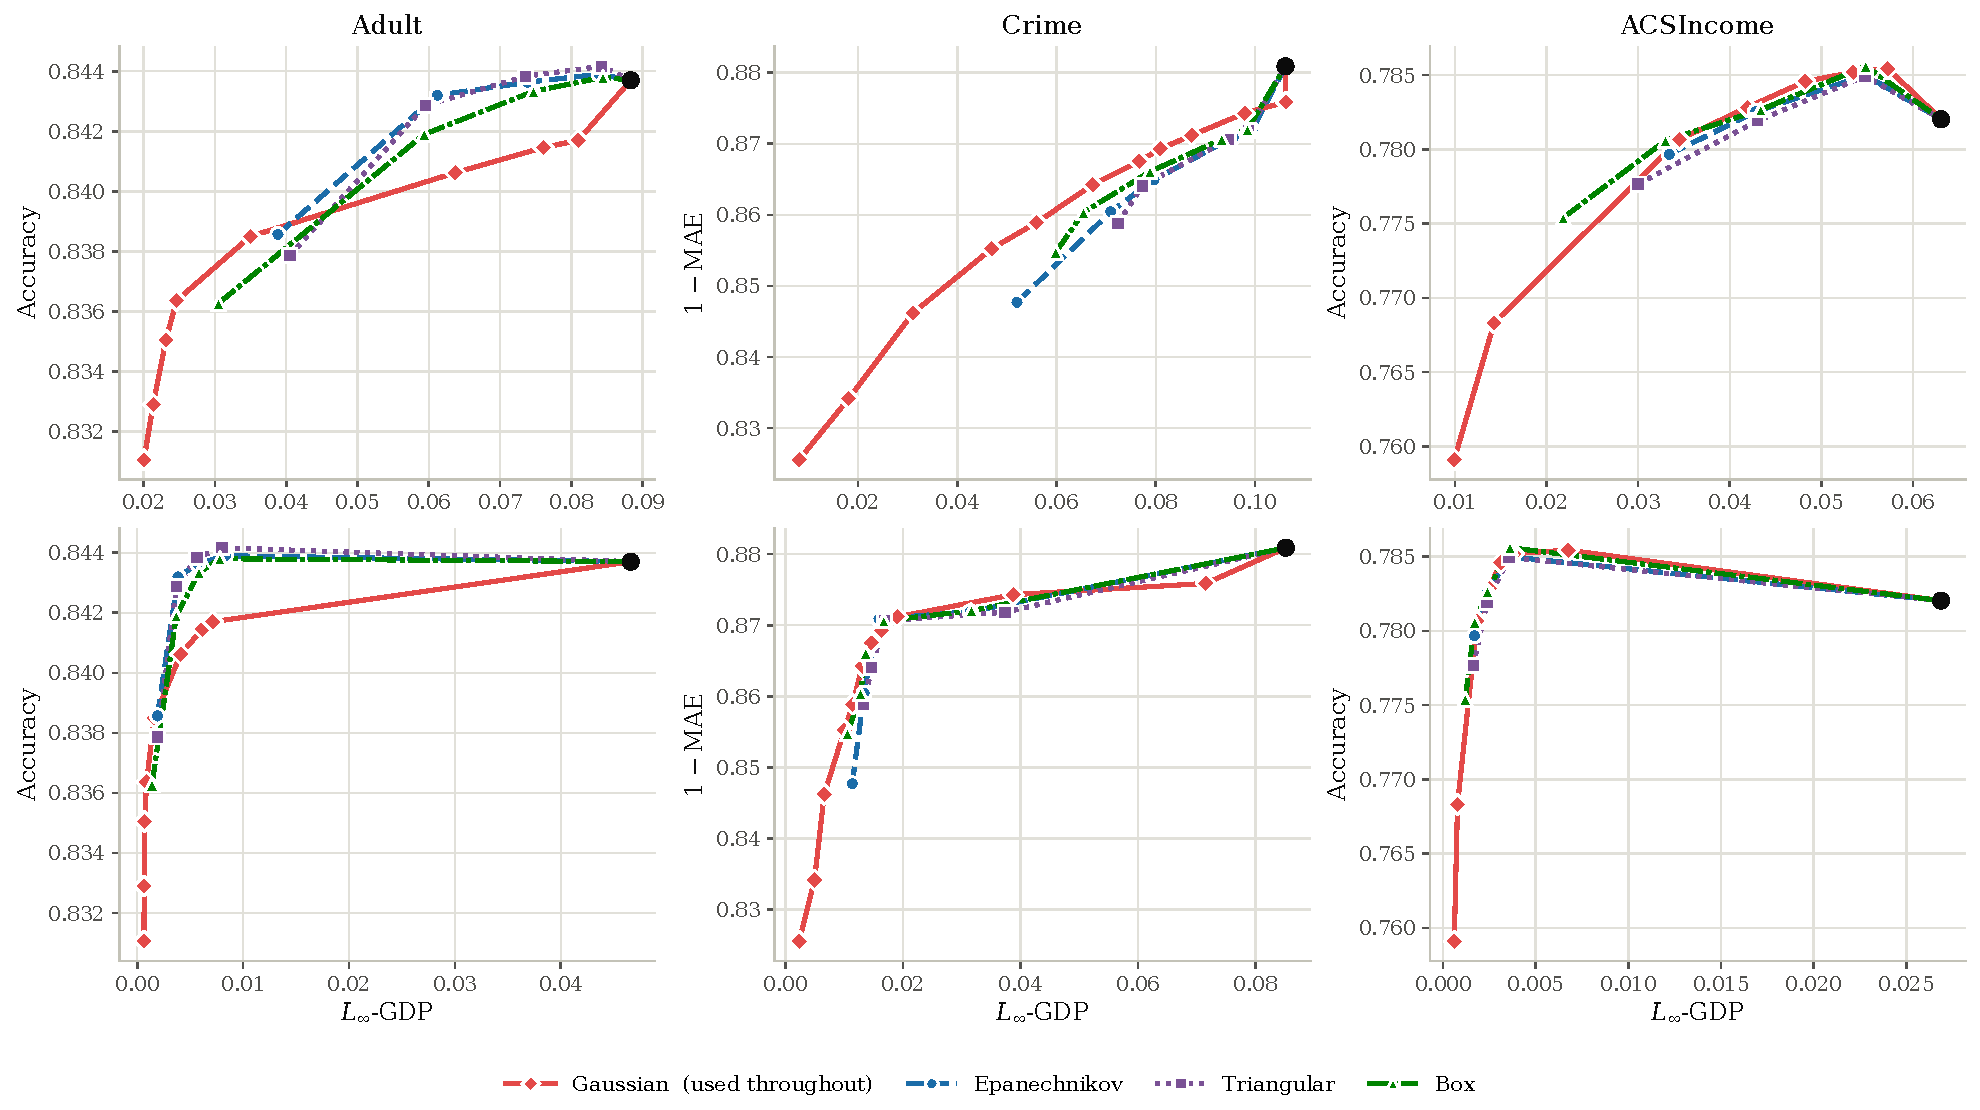
\includegraphics[width=0.92\textwidth]{appendix/figAB_kernel.pdf}
  \caption{Prediction performance against the prediction-level disparity $\widehat{\operatorname{GDP}}_{\infty}(f_{\psi}\circ h_{\phi})$ (top) and the worst-case downstream disparity $\widehat{\operatorname{GDP}}_{\infty}(h_{\phi};\mathcal{F}_{1})$ (bottom) for supIPM-FRL trained with each smoothing kernel, on Adult (left), Crime (middle) and ACSIncome (right).}
  \label{fig:app-ablation-kernel}
\end{figure}
\FloatBarrier

\subsection{IPM Class}
\label{app:ablation-ipm-class}

The discriminator class $\mathcal{V}$ determines which discrepancies between $\mathbb{P}_{\mathbf{Z}\mid S=s}$ and $\mathbb{P}_{\mathbf{Z}}$ the supremum in Equation~(\ref{eq:supipm}) detects, and hence which downstream heads the penalty controls.  We replace the ReLU class $\mathcal{V}_{\mathrm{R}}$ of Equation~(\ref{eq:relu-class}), within the same supremum over $s$, by the sigmoid discriminators $\sigma(\theta^{\top}\mathbf{z}+\mu)$ of sIPM-LFR \citep{kim2022learning} and by the unit ball of the Gaussian RKHS of FREM \citep{kong2025fair}.  The grid of penalty values is chosen separately for each class, since the three IPMs are not on a common scale.

In Figure~\ref{fig:app-ablation-ipm-class}, the three discriminator classes yield similar prediction-level curves.
The ReLU and the sigmoid discriminators attain comparable worst-case disparity, with an ordering that varies with the dataset and the penalty value, and both attain a lower worst-case disparity than the MMD at comparable prediction performance.

\begin{figure}[!htb]
  \centering
  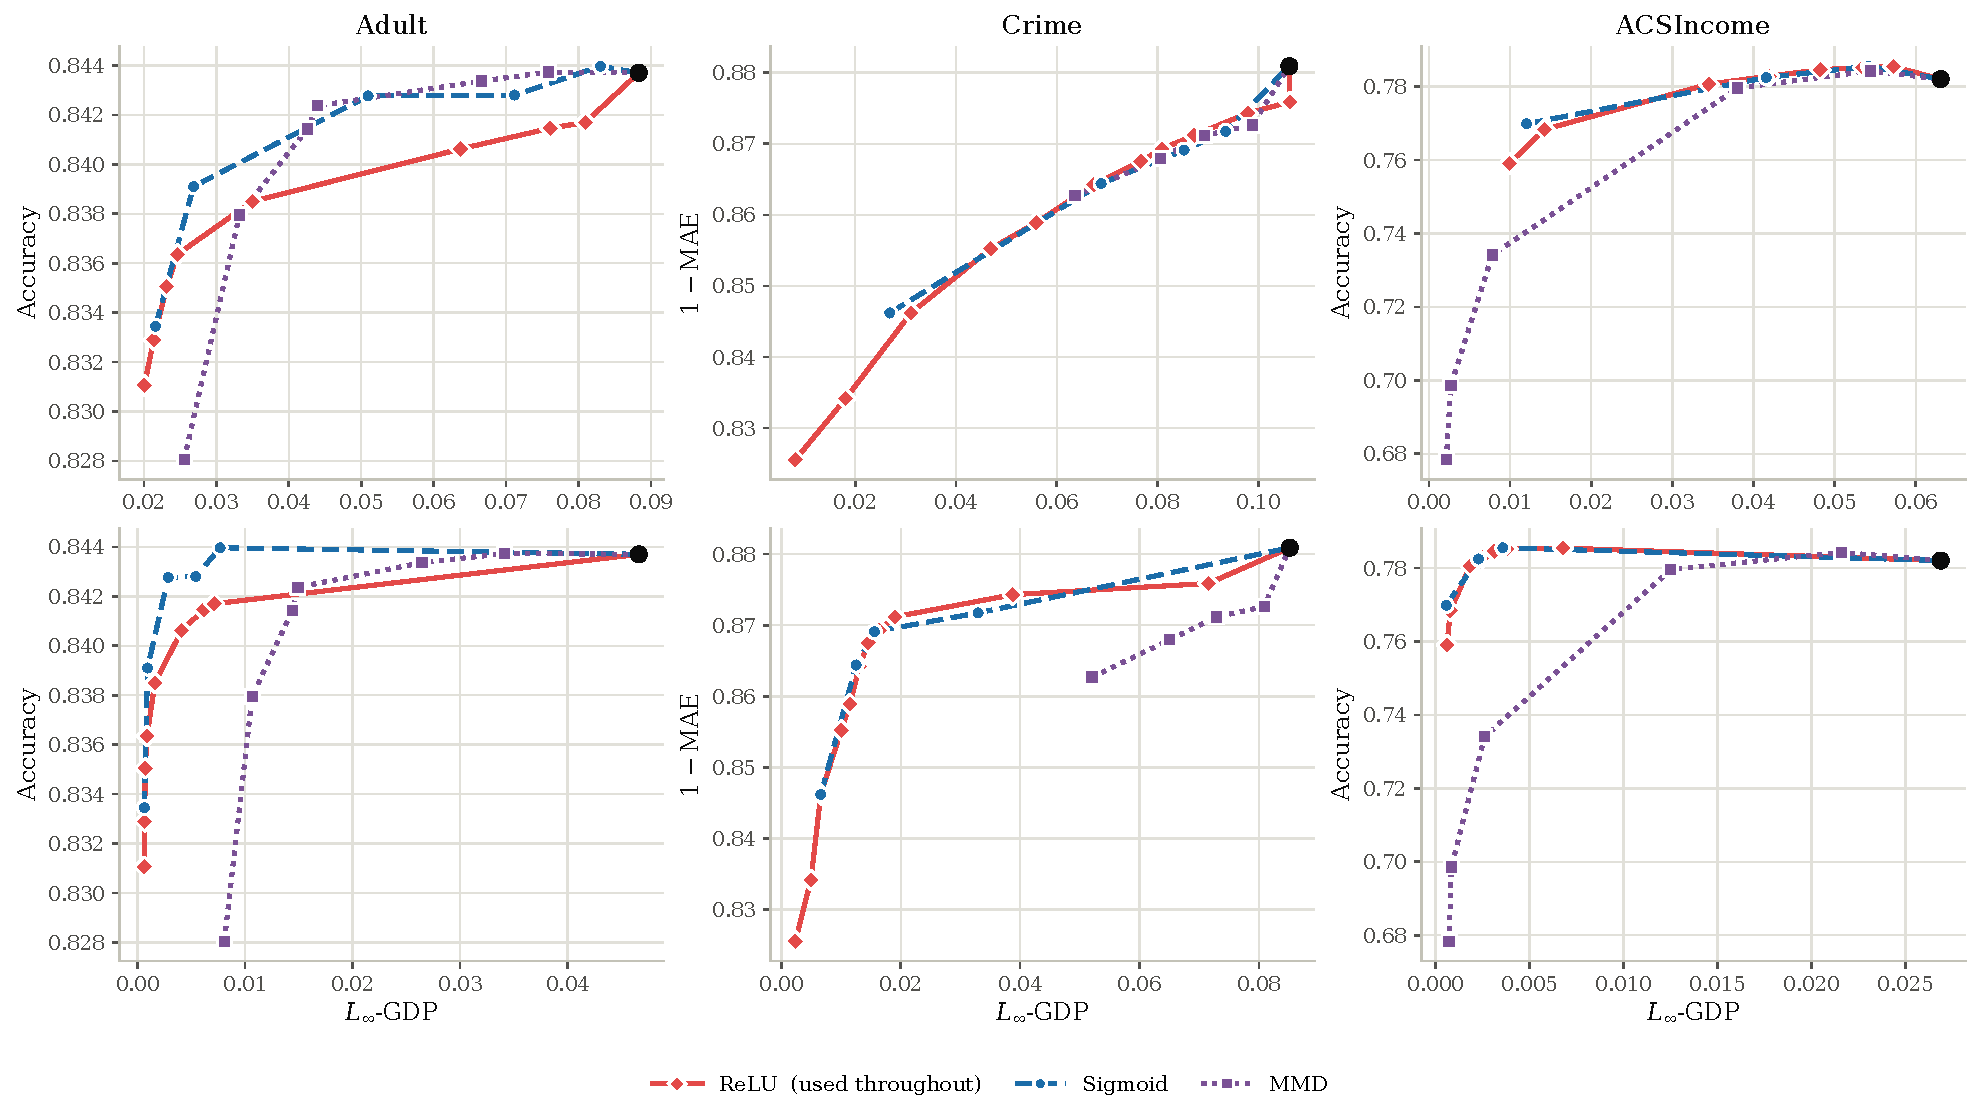
\includegraphics[width=0.92\textwidth]{appendix/figAB_disc.pdf}
  \caption{Prediction performance against the prediction-level disparity $\widehat{\operatorname{GDP}}_{\infty}(f_{\psi}\circ h_{\phi})$ (top) and the worst-case downstream disparity $\widehat{\operatorname{GDP}}_{\infty}(h_{\phi};\mathcal{F}_{1})$ (bottom) for supIPM-FRL trained with each discriminator class, on Adult (left), Crime (middle) and ACSIncome (right).}
  \label{fig:app-ablation-ipm-class}
\end{figure}
\FloatBarrier

\subsection{Candidate Sensitive Values}
\label{app:ablation-T}

The search over $s$ of Appendix~\ref{app:ascent} starts from $T$ candidate sensitive values, so $T$ is how many basins of $\Delta(\cdot\,;\theta,\mu)$ it can find.  This ablation trains supIPM-FRL at $T\in\{5,10,15,20,25,30\}$ alongside the reported $T=17$, and reads every arm on the same seeds and penalty values.

Figure~\ref{fig:app-ablation-T} reports the seven settings.  They are indistinguishable: on Crime the curves coincide, and on Adult and ACSIncome the differences between them lie within one standard deviation over the seeds and show no trend in $T$.

\begin{figure}[!htb]
  \centering
  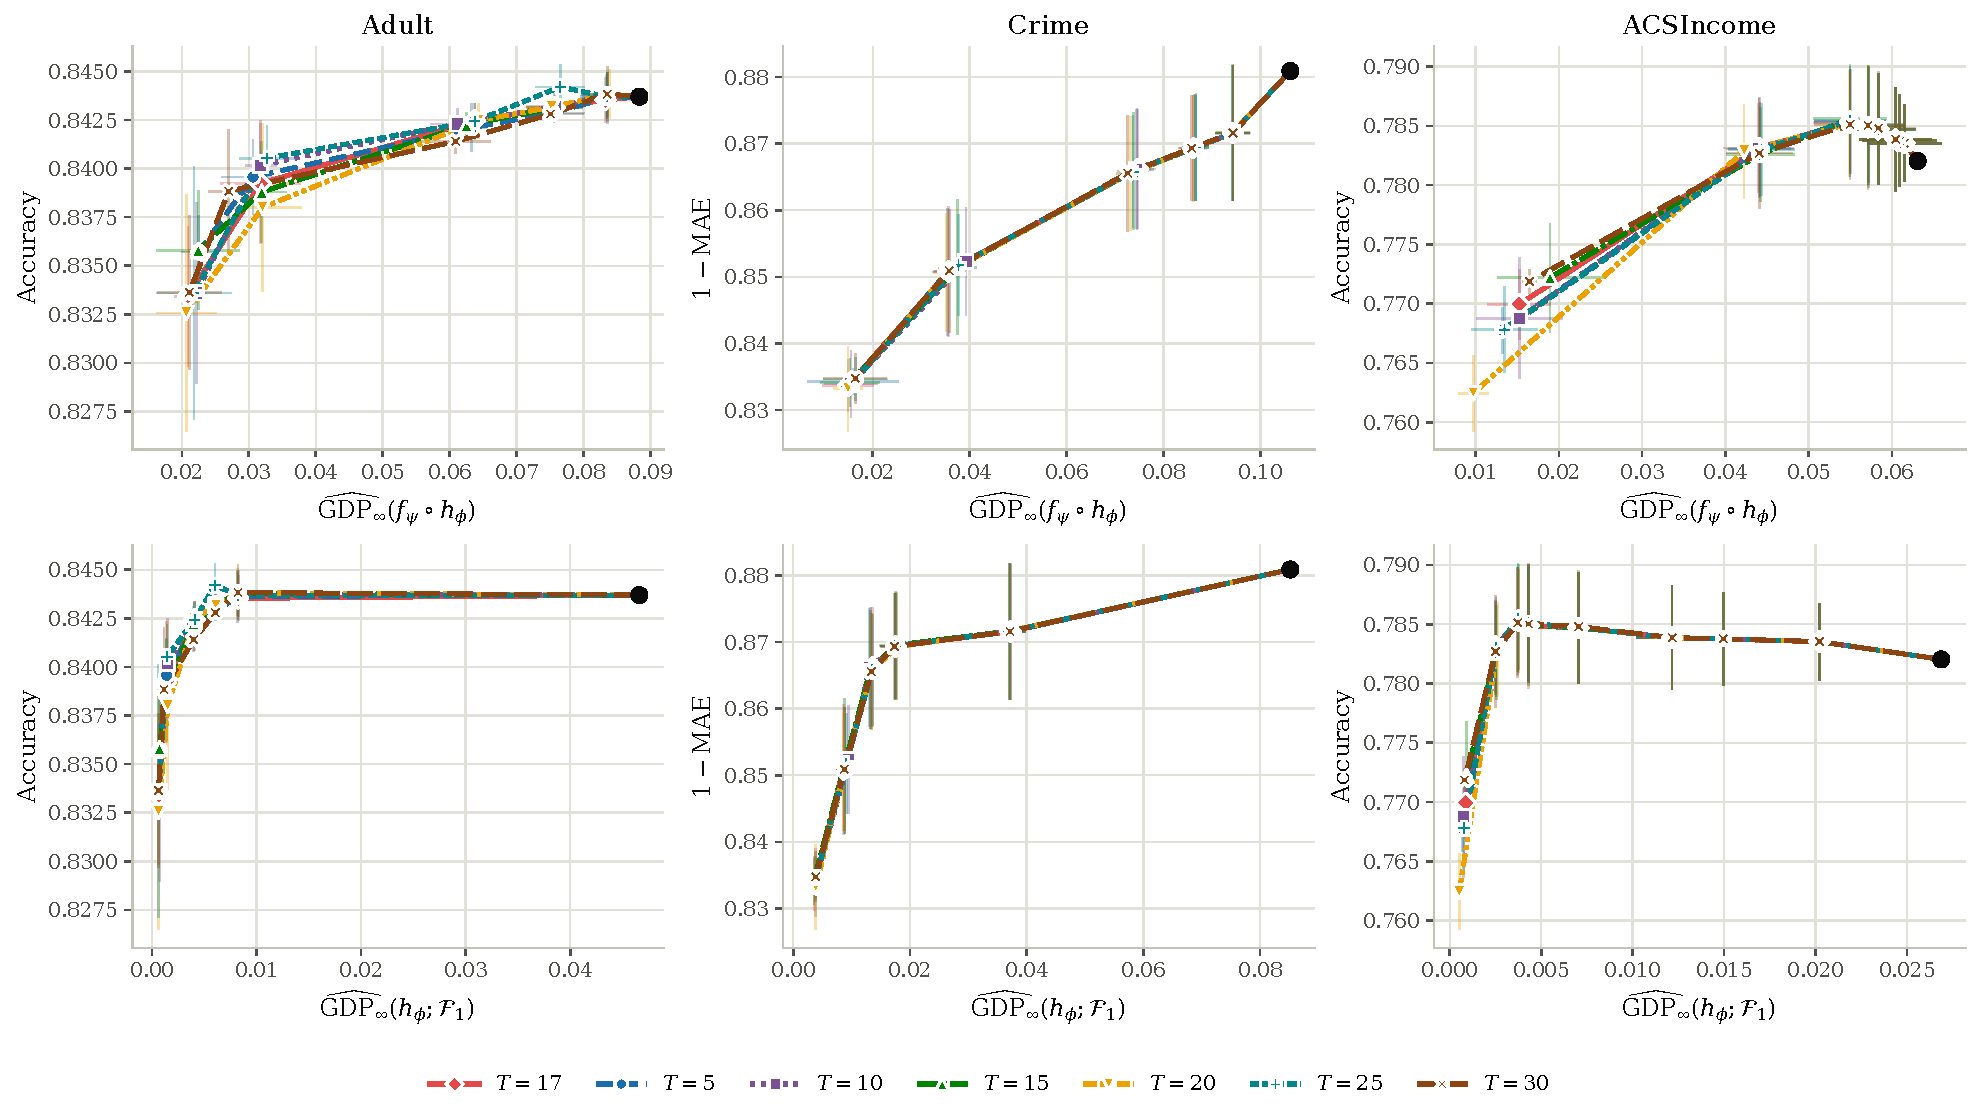
\includegraphics[width=\textwidth]{appendix/figAB_T.pdf}
  \caption{Prediction performance against the prediction-level disparity $\widehat{\operatorname{GDP}}_{\infty}(f_{\psi}\circ h_{\phi})$ (top) and the worst-case downstream disparity $\widehat{\operatorname{GDP}}_{\infty}(h_{\phi};\mathcal{F}_{1})$ (bottom) for supIPM-FRL trained at $T\in\{5,\ldots,30\}$, on Adult (left), Crime (middle) and ACSIncome (right).}
  \label{fig:app-ablation-T}
\end{figure}
\FloatBarrier

\end{document}

\section{Submission of conference papers to ICLR 2027}

ICLR requires electronic submissions, processed by
\url{https://openreview.net/}. See ICLR's website for more instructions.

If your paper is ultimately accepted, the statement {\tt
  {\textbackslash}iclrfinalcopy} should be inserted to adjust the
format to the camera ready requirements.

The format for the submissions is a variant of the NeurIPS format.
Please read carefully the instructions below, and follow them
faithfully.

\subsection{Style}

Papers to be submitted to ICLR 2027 must be prepared according to the
instructions presented here.

%% Please note that we have introduced automatic line number generation
%% into the style file for \LaTeXe. This is to help reviewers
%% refer to specific lines of the paper when they make their comments. Please do
%% NOT refer to these line numbers in your paper as they will be removed from the
%% style file for the final version of accepted papers.

Authors are required to use the ICLR \LaTeX{} style files obtainable at the
ICLR website. Please make sure you use the current files and
not previous versions. Tweaking the style files may be grounds for rejection.

\subsection{Retrieval of style files}

The style files for ICLR and other conference information are available online at:
\begin{center}
   \url{http://www.iclr.cc/}
\end{center}
The file \verb+iclr2027_conference.pdf+ contains these
instructions and illustrates the
various formatting requirements your ICLR paper must satisfy.
Submissions must be made using \LaTeX{} and the style files
\verb+iclr2027_conference.sty+ and \verb+iclr2027_conference.bst+ (to be used with \LaTeX{}2e). The file
\verb+iclr2027_conference.tex+ may be used as a ``shell'' for writing your paper. All you
have to do is replace the author, title, abstract, and text of the paper with
your own.

The formatting instructions contained in these style files are summarized in
sections \ref{gen_inst}, \ref{headings}, and \ref{others} below.

\section{General formatting instructions}
\label{gen_inst}

The text must be confined within a rectangle 5.5~inches (33~picas) wide and
9~inches (54~picas) long. The left margin is 1.5~inch (9~picas).
Use 10~point type with a vertical spacing of 11~points. Times New Roman is the
preferred typeface throughout. Paragraphs are separated by 1/2~line space,
with no indentation.

Paper title is 17~point, in small caps and left-aligned.
All pages should start at 1~inch (6~picas) from the top of the page.

Authors' names are
set in boldface, and each name is placed above its corresponding
address. The lead author's name is to be listed first, and
the co-authors' names are set to follow. Authors sharing the
same address can be on the same line.

Please pay special attention to the instructions in section \ref{others}
regarding figures, tables, acknowledgments, and references.


There will be a strict upper limit of \textbf{9 pages} for the main text of the initial submission, with unlimited additional pages for citations. This limit will be expanded to \textbf{10 pages} for rebuttal/camera ready.

\section{Headings: first level}
\label{headings}

First level headings are in small caps,
flush left and in point size 12. One line space before the first level
heading and 1/2~line space after the first level heading.

\subsection{Headings: second level}

Second level headings are in small caps,
flush left and in point size 10. One line space before the second level
heading and 1/2~line space after the second level heading.

\subsubsection{Headings: third level}

Third level headings are in small caps,
flush left and in point size 10. One line space before the third level
heading and 1/2~line space after the third level heading.

\section{Citations, figures, tables, references}
\label{others}

These instructions apply to everyone, regardless of the formatter being used.

\subsection{Citations within the text}

Citations within the text should be based on the \texttt{natbib} package
and include the authors' last names and year (with the ``et~al.'' construct
for more than two authors). When the authors or the publication are
included in the sentence, the citation should not be in parenthesis using \verb|\citet{}| (as
in ``See \citet{Hinton06} for more information.''). Otherwise, the citation
should be in parenthesis using \verb|\citep{}| (as in ``Deep learning shows promise to make progress
towards AI~\citep{Bengio+chapter2007}.'').

The corresponding references are to be listed in alphabetical order of
authors, in the \textsc{References} section. As to the format of the
references themselves, any style is acceptable as long as it is used
consistently.

\subsection{Footnotes}

Indicate footnotes with a number\footnote{Sample of the first footnote} in the
text. Place the footnotes at the bottom of the page on which they appear.
Precede the footnote with a horizontal rule of 2~inches
(12~picas).\footnote{Sample of the second footnote}

\subsection{Figures}

All artwork must be neat, clean, and legible. Lines should be dark
enough for purposes of reproduction; art work should not be
hand-drawn. The figure number and caption always appear after the
figure. Place one line space before the figure caption, and one line
space after the figure. The figure caption is lower case (except for
first word and proper nouns); figures are numbered consecutively.

Make sure the figure caption does not get separated from the figure.
Leave sufficient space to avoid splitting the figure and figure caption.

You may use color figures.
However, it is best for the
figure captions and the paper body to make sense if the paper is printed
either in black/white or in color.
\begin{figure}[h]
\begin{center}
%\framebox[4.0in]{$\;$}
\fbox{\rule[-.5cm]{0cm}{4cm} \rule[-.5cm]{4cm}{0cm}}
\end{center}
\caption{Sample figure caption.}
\end{figure}

\subsection{Tables}

All tables must be centered, neat, clean and legible. Do not use hand-drawn
tables. The table number and title always appear before the table. See
Table~\ref{sample-table}.

Place one line space before the table title, one line space after the table
title, and one line space after the table. The table title must be lower case
(except for first word and proper nouns); tables are numbered consecutively.

\begin{table}[t]
\caption{Sample table title}
\label{sample-table}
\begin{center}
\begin{tabular}{ll}
\multicolumn{1}{c}{\bf PART}  &\multicolumn{1}{c}{\bf DESCRIPTION}
\\ \hline \\
Dendrite         &Input terminal \\
Axon             &Output terminal \\
Soma             &Cell body (contains cell nucleus) \\
\end{tabular}
\end{center}
\end{table}

\section{Default Notation}

In an attempt to encourage standardized notation, we have included the
notation file from the textbook, \textit{Deep Learning}
\cite{goodfellow2016deep} available at
\url{https://github.com/goodfeli/dlbook_notation/}.  Use of this style
is not required and can be disabled by commenting out
\texttt{math\_commands.tex}.


\centerline{\bf Numbers and Arrays}
\bgroup
\def\arraystretch{1.5}
\begin{tabular}{p{1in}p{3.25in}}
$\displaystyle a$ & A scalar (integer or real)\\
$\displaystyle \va$ & A vector\\
$\displaystyle \mA$ & A matrix\\
$\displaystyle \tA$ & A tensor\\
$\displaystyle \mI_n$ & Identity matrix with $n$ rows and $n$ columns\\
$\displaystyle \mI$ & Identity matrix with dimensionality implied by context\\
$\displaystyle \ve^{(i)}$ & Standard basis vector $[0,\dots,0,1,0,\dots,0]$ with a 1 at position $i$\\
$\displaystyle \text{diag}(\va)$ & A square, diagonal matrix with diagonal entries given by $\va$\\
$\displaystyle \ra$ & A scalar random variable\\
$\displaystyle \rva$ & A vector-valued random variable\\
$\displaystyle \rmA$ & A matrix-valued random variable\\
\end{tabular}
\egroup
\vspace{0.25cm}

\centerline{\bf Sets and Graphs}
\bgroup
\def\arraystretch{1.5}

\begin{tabular}{p{1.25in}p{3.25in}}
$\displaystyle \sA$ & A set\\
$\displaystyle \R$ & The set of real numbers \\
$\displaystyle \{0, 1\}$ & The set containing 0 and 1 \\
$\displaystyle \{0, 1, \dots, n \}$ & The set of all integers between $0$ and $n$\\
$\displaystyle [a, b]$ & The real interval including $a$ and $b$\\
$\displaystyle (a, b]$ & The real interval excluding $a$ but including $b$\\
$\displaystyle \sA \backslash \sB$ & Set subtraction, i.e., the set containing the elements of $\sA$ that are not in $\sB$\\
$\displaystyle \gG$ & A graph\\
$\displaystyle \parents_\gG(\ervx_i)$ & The parents of $\ervx_i$ in $\gG$
\end{tabular}
\vspace{0.25cm}


\centerline{\bf Indexing}
\bgroup
\def\arraystretch{1.5}

\begin{tabular}{p{1.25in}p{3.25in}}
$\displaystyle \eva_i$ & Element $i$ of vector $\va$, with indexing starting at 1 \\
$\displaystyle \eva_{-i}$ & All elements of vector $\va$ except for element $i$ \\
$\displaystyle \emA_{i,j}$ & Element $i, j$ of matrix $\mA$ \\
$\displaystyle \mA_{i, :}$ & Row $i$ of matrix $\mA$ \\
$\displaystyle \mA_{:, i}$ & Column $i$ of matrix $\mA$ \\
$\displaystyle \etA_{i, j, k}$ & Element $(i, j, k)$ of a 3-D tensor $\tA$\\
$\displaystyle \tA_{:, :, i}$ & 2-D slice of a 3-D tensor\\
$\displaystyle \erva_i$ & Element $i$ of the random vector $\rva$ \\
\end{tabular}
\egroup
\vspace{0.25cm}


\centerline{\bf Calculus}
\bgroup
\def\arraystretch{1.5}
\begin{tabular}{p{1.25in}p{3.25in}}
% NOTE: the [2ex] on the next line adds extra height to that row of the table.
% Without that command, the fraction on the first line is too tall and collides
% with the fraction on the second line.
$\displaystyle\frac{d y} {d x}$ & Derivative of $y$ with respect to $x$\\ [2ex]
$\displaystyle \frac{\partial y} {\partial x} $ & Partial derivative of $y$ with respect to $x$ \\
$\displaystyle \nabla_\vx y $ & Gradient of $y$ with respect to $\vx$ \\
$\displaystyle \nabla_\mX y $ & Matrix derivatives of $y$ with respect to $\mX$ \\
$\displaystyle \nabla_\tX y $ & Tensor containing derivatives of $y$ with respect to $\tX$ \\
$\displaystyle \frac{\partial f}{\partial \vx} $ & Jacobian matrix $\mJ \in \R^{m\times n}$ of $f: \R^n \rightarrow \R^m$\\
$\displaystyle \nabla_\vx^2 f(\vx)\text{ or }\mH( f)(\vx)$ & The Hessian matrix of $f$ at input point $\vx$\\
$\displaystyle \int f(\vx) d\vx $ & Definite integral over the entire domain of $\vx$ \\
$\displaystyle \int_\sS f(\vx) d\vx$ & Definite integral with respect to $\vx$ over the set $\sS$ \\
\end{tabular}
\egroup
\vspace{0.25cm}

\centerline{\bf Probability and Information Theory}
\bgroup
\def\arraystretch{1.5}
\begin{tabular}{p{1.25in}p{3.25in}}
$\displaystyle P(\ra)$ & A probability distribution over a discrete variable\\
$\displaystyle p(\ra)$ & A probability distribution over a continuous variable, or over
a variable whose type has not been specified\\
$\displaystyle \ra \sim P$ & Random variable $\ra$ has distribution $P$\\% so thing on left of \sim should always be a random variable, with name beginning with \r
$\displaystyle  \E_{\rx\sim P} [ f(x) ]\text{ or } \E f(x)$ & Expectation of $f(x)$ with respect to $P(\rx)$ \\
$\displaystyle \Var(f(x)) $ &  Variance of $f(x)$ under $P(\rx)$ \\
$\displaystyle \Cov(f(x),g(x)) $ & Covariance of $f(x)$ and $g(x)$ under $P(\rx)$\\
$\displaystyle H(\rx) $ & Shannon entropy of the random variable $\rx$\\
$\displaystyle \KL ( P \Vert Q ) $ & Kullback-Leibler divergence of P and Q \\
$\displaystyle \mathcal{N} ( \vx ; \vmu , \mSigma)$ & Gaussian distribution %
over $\vx$ with mean $\vmu$ and covariance $\mSigma$ \\
\end{tabular}
\egroup
\vspace{0.25cm}

\centerline{\bf Functions}
\bgroup
\def\arraystretch{1.5}
\begin{tabular}{p{1.25in}p{3.25in}}
$\displaystyle f: \sA \rightarrow \sB$ & The function $f$ with domain $\sA$ and range $\sB$\\
$\displaystyle f \circ g $ & Composition of the functions $f$ and $g$ \\
  $\displaystyle f(\vx ; \vtheta) $ & A function of $\vx$ parametrized by $\vtheta$.
  (Sometimes we write $f(\vx)$ and omit the argument $\vtheta$ to lighten notation) \\
$\displaystyle \log x$ & Natural logarithm of $x$ \\
$\displaystyle \sigma(x)$ & Logistic sigmoid, $\displaystyle \frac{1} {1 + \exp(-x)}$ \\
$\displaystyle \zeta(x)$ & Softplus, $\log(1 + \exp(x))$ \\
$\displaystyle || \vx ||_p $ & $\normlp$ norm of $\vx$ \\
$\displaystyle || \vx || $ & $\normltwo$ norm of $\vx$ \\
$\displaystyle x^+$ & Positive part of $x$, i.e., $\max(0,x)$\\
$\displaystyle \1_\mathrm{condition}$ & is 1 if the condition is true, 0 otherwise\\
\end{tabular}
\egroup
\vspace{0.25cm}


\section{Final instructions}
Do not change any aspects of the formatting parameters in the style files.
In particular, do not modify the width or length of the rectangle the text
should fit into, and do not change font sizes (except perhaps in the
\textsc{References} section; see below). Please note that pages should be
numbered.

\section{Preparing PostScript or PDF files}

Please prepare PostScript or PDF files with paper size ``US Letter'', and
not, for example, ``A4''. The -t
letter option on dvips will produce US Letter files.

Consider directly generating PDF files using \verb+pdflatex+
(especially if you are a MiKTeX user).
PDF figures must be substituted for EPS figures, however.

Otherwise, please generate your PostScript and PDF files with the following commands:
\begin{verbatim}
dvips mypaper.dvi -t letter -Ppdf -G0 -o mypaper.ps
ps2pdf mypaper.ps mypaper.pdf
\end{verbatim}

\subsection{Margins in LaTeX}

Most of the margin problems come from figures positioned by hand using
\verb+\special+ or other commands. We suggest using the command
\verb+\includegraphics+
from the graphicx package. Always specify the figure width as a multiple of
the line width as in the example below using .eps graphics
\begin{verbatim}
   \usepackage[dvips]{graphicx} ...
   \includegraphics[width=0.8\linewidth]{myfile.eps}
\end{verbatim}
or % Apr 2009 addition
\begin{verbatim}
   \usepackage[pdftex]{graphicx} ...
   \includegraphics[width=0.8\linewidth]{myfile.pdf}
\end{verbatim}
for .pdf graphics.
See section~4.4 in the graphics bundle documentation (\url{http://www.ctan.org/tex-archive/macros/latex/required/graphics/grfguide.ps})

A number of width problems arise when LaTeX cannot properly hyphenate a
line. Please give LaTeX hyphenation hints using the \verb+\-+ command.

\subsection*{AI use statement}

(This section is \textbf{required} and does not count toward the page limit.)

In this work, we used generative AI tools for [tasks with required disclosure].
We have not used generative AI tools for [other tasks with required disclosure],
and [the rest of the required disclosure tasks] are not applicable to this work.
Additionally, we used generative AI tools for [tasks with recommended
disclosure]. We have reviewed all AI-assisted work. [Elaborate. For example, “we
checked LLM-generated research ideas for potential plagiarism through a manual
literature survey”, “LLM-generated code was verified and tested for correctness
by 2 authors”, etc.]. We take responsibility for the final content of this work,
including text, claims or artifacts produced with the aid of generative AI.

See the ICLR 2027 AI Policy for Authors for more details. This statement should
not be more than 1 page.

\subsection*{Ethics statement}

(This section is \textbf{recommended} and does not count toward the page limit.)

If authors feel that their paper submission raises questions regarding the Code
of Ethics, they are encouraged to include a paragraph of Ethics Statement (at
the end of the main text before references) to address potential concerns where
appropriate. Topics include, but are not limited to, studies that involve human
subjects, practices to data set releases, potentially harmful insights,
methodologies and applications, potential conflicts of interest and sponsorship,
discrimination/bias/fairness concerns, privacy and security issues, legal
compliance, and research integrity issues (e.g., IRB, documentation, research
ethics). This statement should not be more than 1 page.

\subsection*{Reproducibility statement}

(This section is \textbf{recommended} and does not count toward the page limit.)

It is important that the work published in ICLR is reproducible. Authors are
strongly encouraged to include a paragraph-long Reproducibility Statement at the
end of the main text (before references) to discuss the efforts that have been
made to ensure reproducibility. This paragraph should not itself describe
details needed for reproducing the results, but rather reference the parts of
the main paper, appendix, and supplemental materials that will help with
reproducibility. For example, for novel models or algorithms, a link to an
anonymous downloadable source code can be submitted as supplementary materials;
for theoretical results, clear explanations of any assumptions and a complete
proof of the claims can be included in the appendix; for any datasets used in
the experiments, a complete description of the data processing steps can be
provided in the supplementary materials. Each of the above are examples of
things that can be referenced in the reproducibility statement.

\subsubsection*{Author Contributions}
If you'd like to, you may include  a section for author contributions as is done
in many journals. This is optional and at the discretion of the authors.

\subsubsection*{Acknowledgments}
Use unnumbered third level headings for the acknowledgments. All
acknowledgments, including those to funding agencies, go at the end of the paper.


\bibliography{iclr2027_conference}
\bibliographystyle{iclr2027_conference}

\appendix
\section{Appendix}
You may include other additional sections here.


\end{document}
